\section{Controllers}
To test the different controllers a set of positions were chosen as target reaching positions. These points can be seen in the Figure \ref{fig:desiredpoints}. The initial position is marked in red and the target positions are marked in blue.

\begin{figure}[h!] 
    \centering
    \begin{subfigure}[b]{0.45\linewidth}
        \centering

        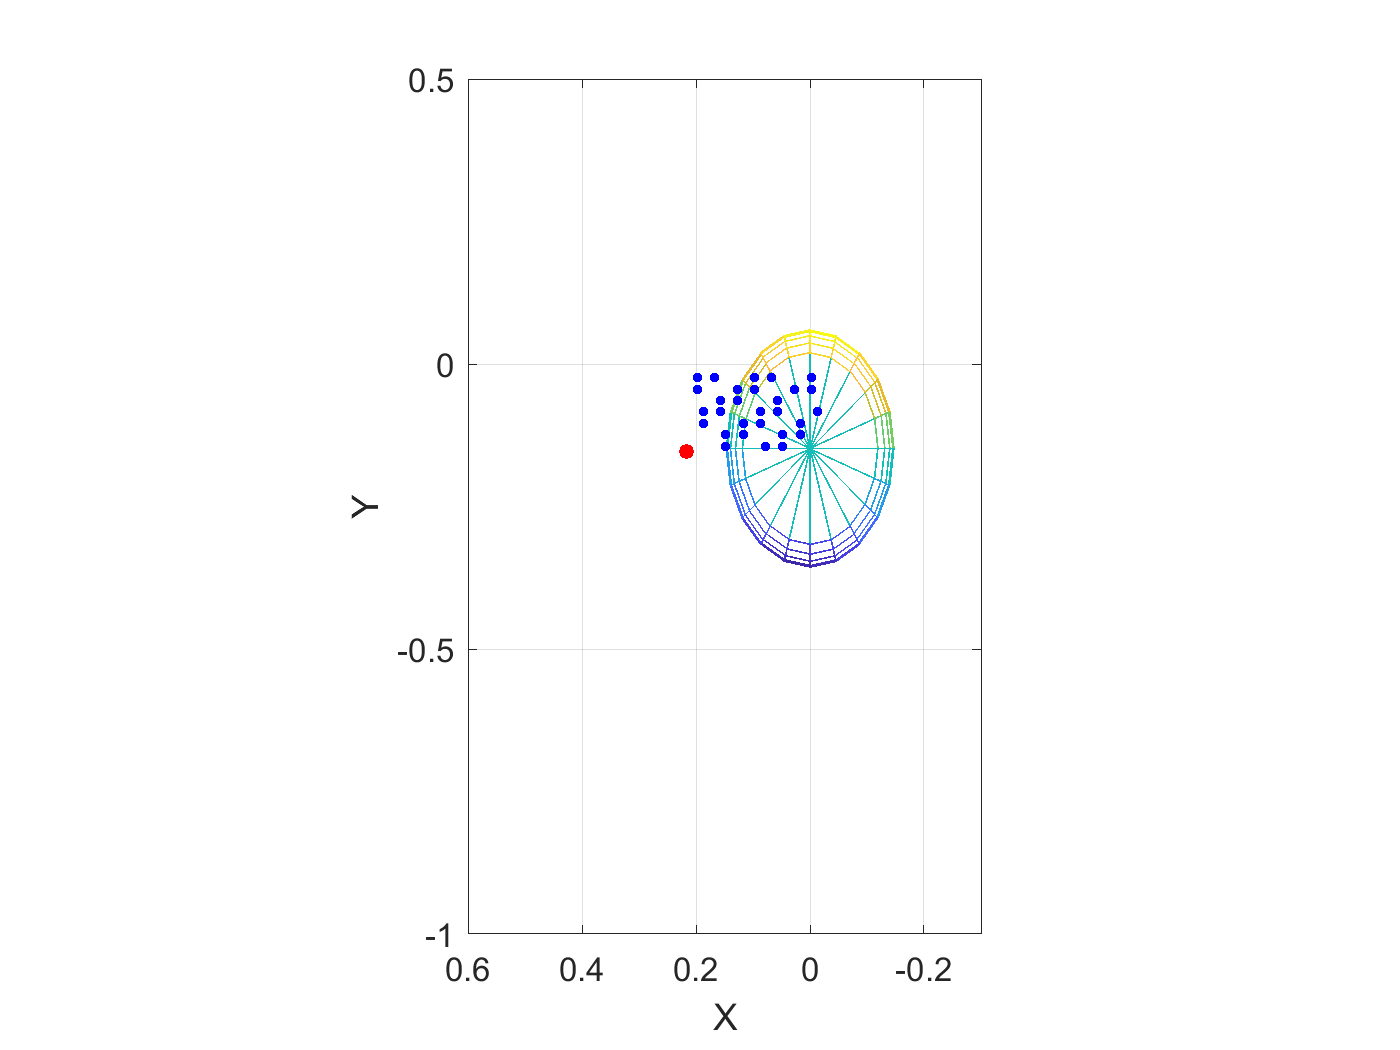
\includegraphics[width=0.7\textwidth]{Pictures/Results/Controller/DesiredPointsFV.png}
    \end{subfigure}
    \hfill
    %\vspace{1cm} % Adjust the space between the figures as needed
    \begin{subfigure}[b]{0.45\linewidth}       
        \centering

        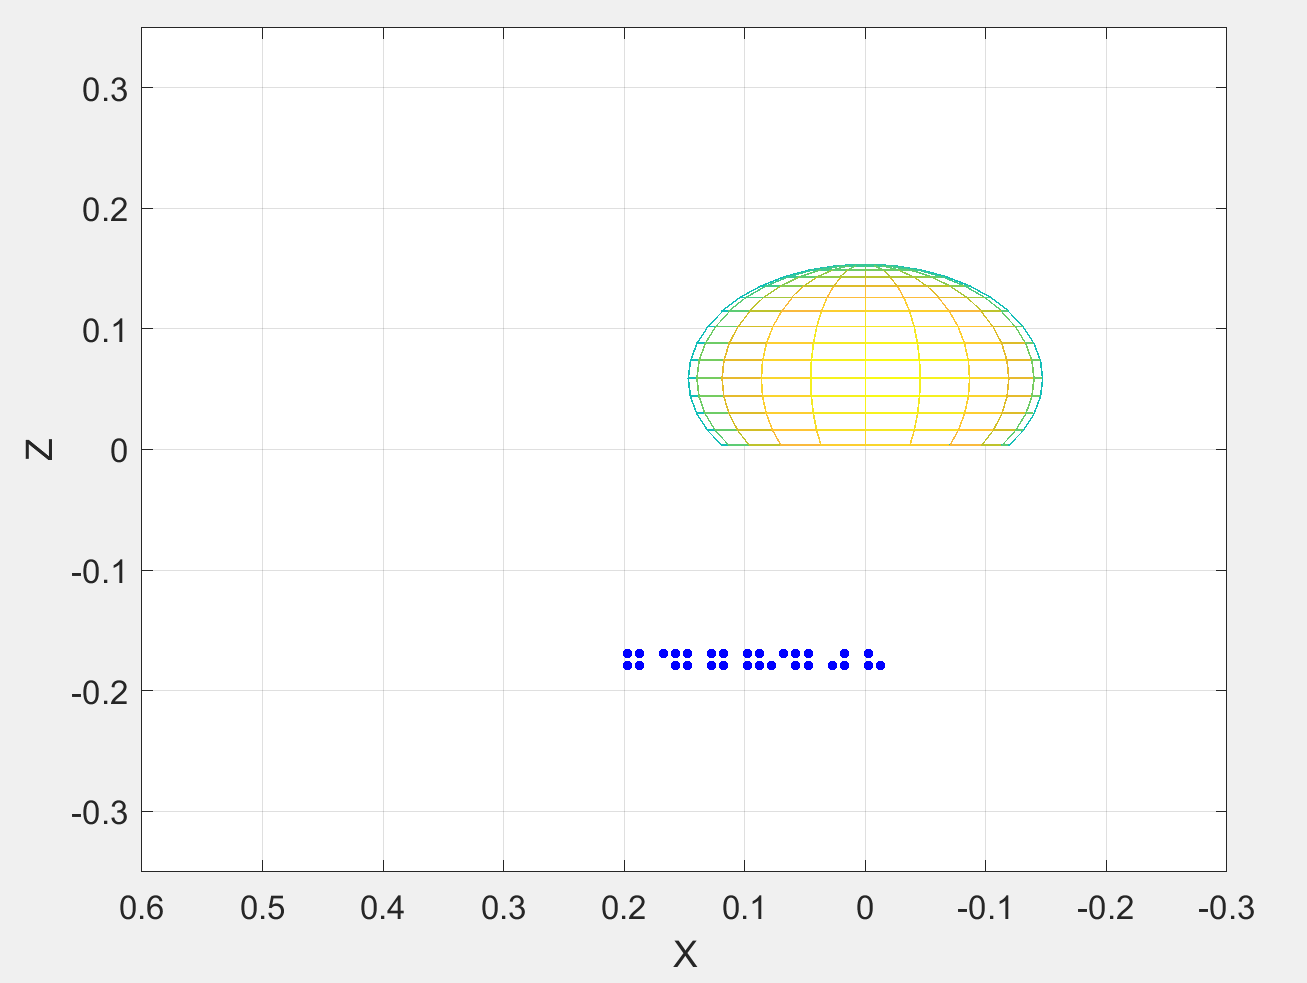
\includegraphics[width=0.7\textwidth]{Pictures/Results/Controller/DesiredPointsSV.png}
    \end{subfigure}
    \caption{Desired Targets for Reaching in Rehabilitation Task (Front View, Side View)}
    \label{fig:desiredpoints}
\end{figure}

Figure \ref{fig:allcontrollers} provides an initial overview of the different controllers operating at the same point. The progression begins with the static controller, transitions to path-following for the target point, and then introduces the stroke factor, affecting the arm's movement. In the final layer, the EMG-Influenced FES controller is integrated with the stroke-affected movement, allowing the arm to execute motions similar to those in a non-stroke scenario.

\begin{figure}[ht]
    \centering

    % Row 1, Column 1
    \begin{subfigure}[b]{0.5\textwidth}
        \centering

        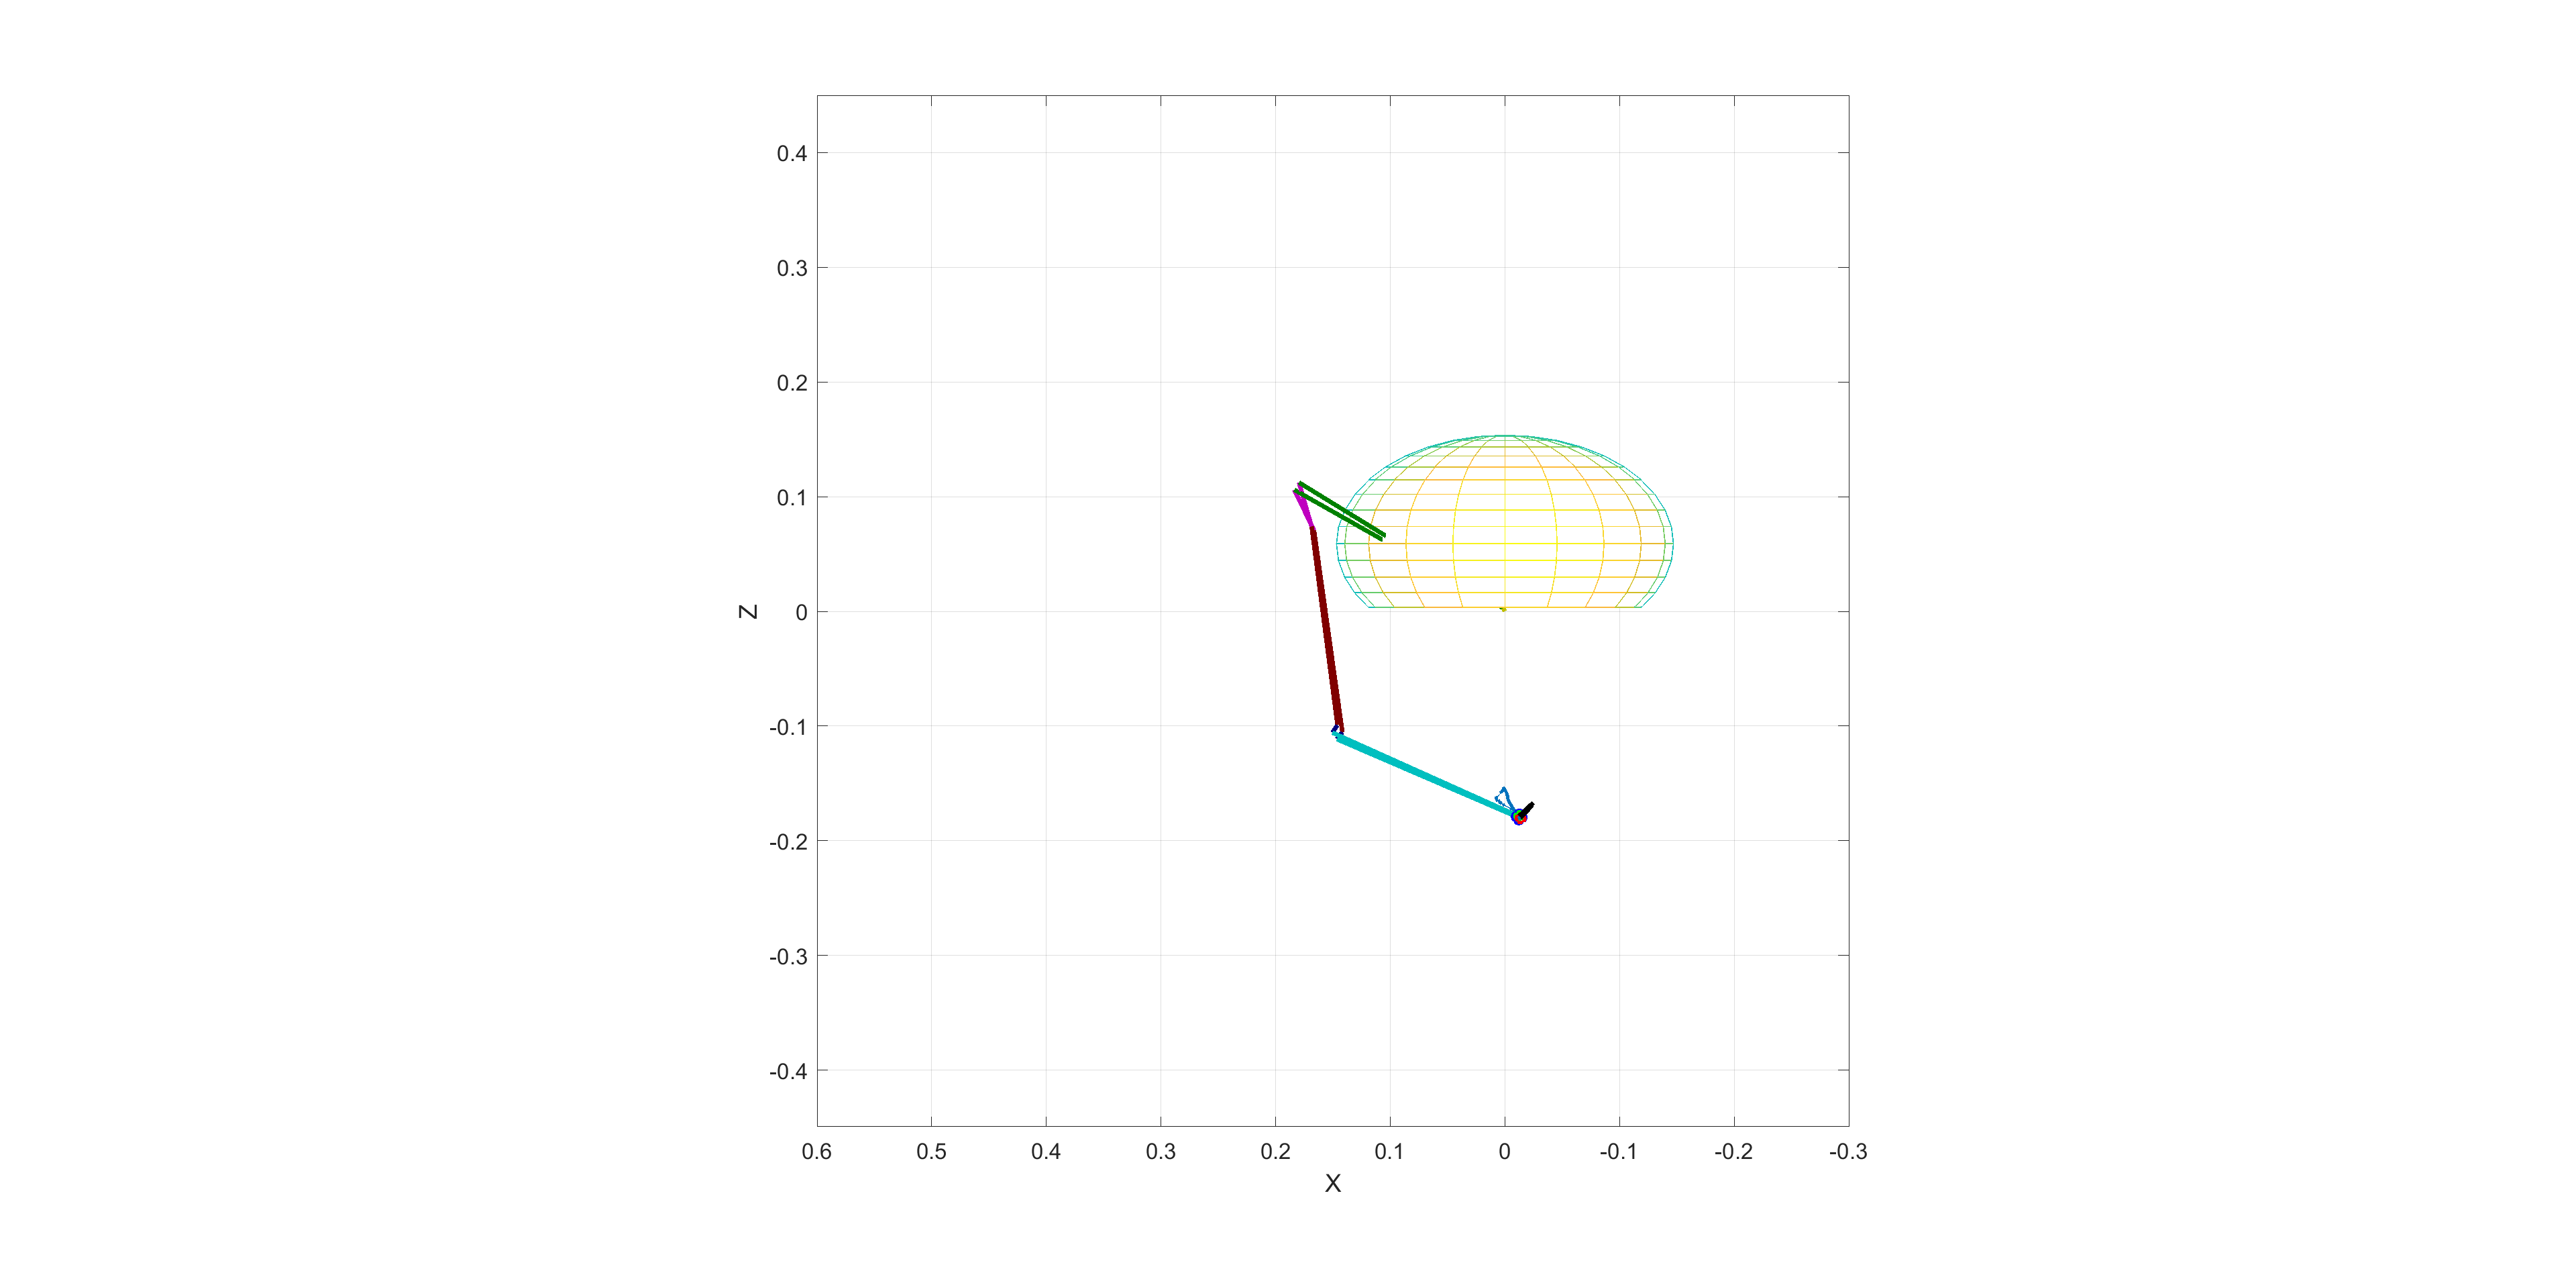
\includegraphics[width=0.75\linewidth]{Pictures/Controller/StaticControl_WP.png}
        \caption{Static Controller                                   }
    \end{subfigure}%
    \hfill
    % Row 1, Column 2
    \begin{subfigure}[b]{0.5\textwidth}
        \centering

        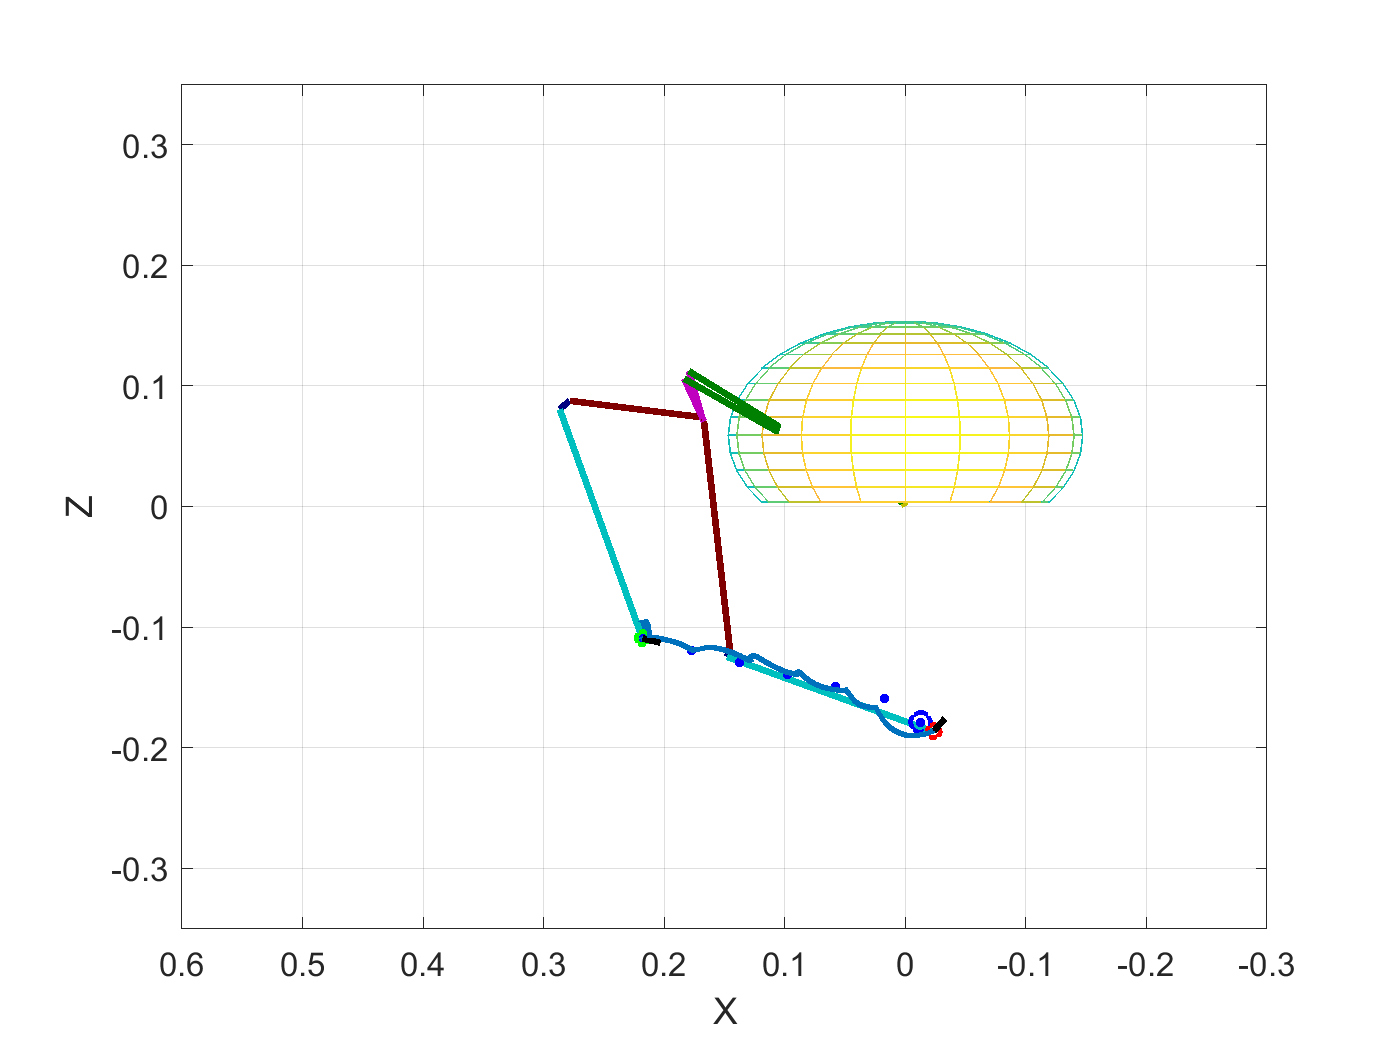
\includegraphics[width=0.75\linewidth]{Pictures/Results/Controller/Healthy_WP.png}
        \caption{Non-Stroke Path-Following Quasi-Static Controller}
    \end{subfigure}

    \vspace{2pt} % Some vertical space between the rows

    % Row 2, Column 1
    \begin{subfigure}[b]{0.5\textwidth}
        \centering

        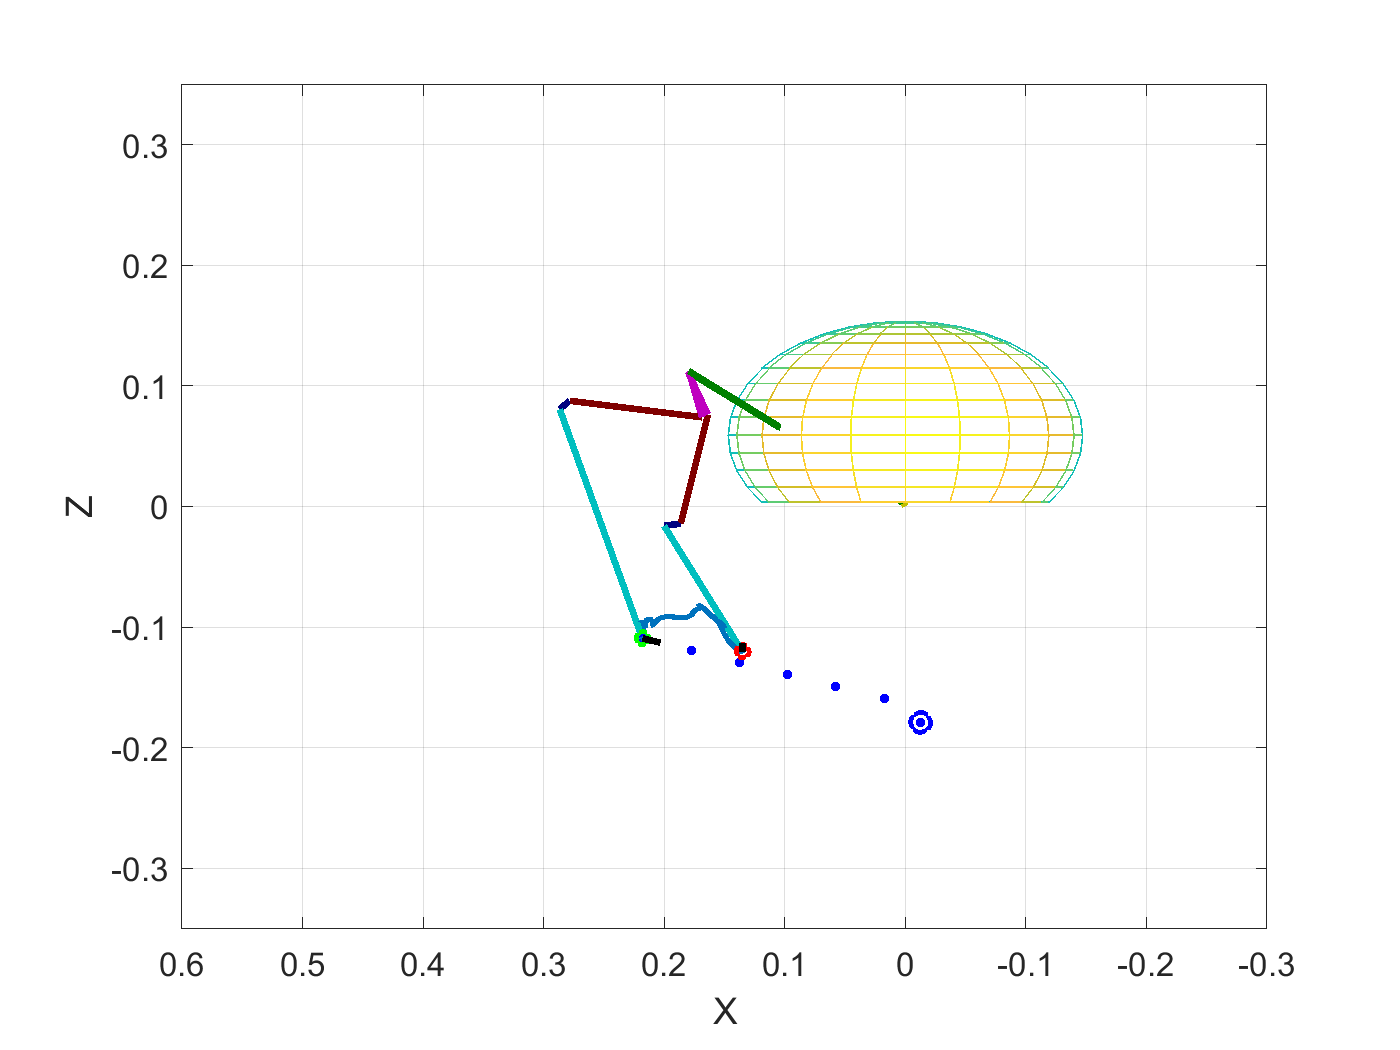
\includegraphics[width=0.75\linewidth]{Pictures/Results/Controller/StrokeWithouControl_WP.png}
        \caption{Stroke Path-Following Quasi-Static Controller}
    \end{subfigure}%
    \hfill
    % Row 2, Column 2
    \begin{subfigure}[b]{0.5\textwidth}
        \centering

        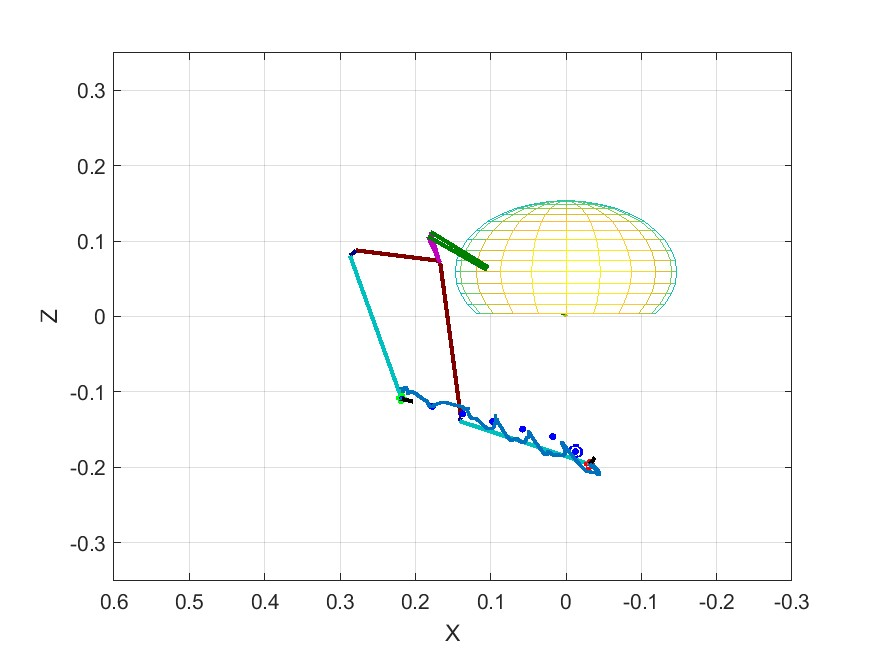
\includegraphics[width=0.75\linewidth]{Pictures/Results/Controller/G(2.99)_G(14.48)_Stroke_7_position_totry(5485)_wp.jpg}
        \caption{Stroke EMG-Influenced Quasi-Static Controller}
    \end{subfigure}

    \caption{Wrist Position Plots over Time}
    \label{fig:allcontrollers}
\end{figure}

\newpage
\subsection{Static Controller} \label{resultsstaticcontrol}
The PI tuning for the static controller was done with half of the desired points. However, the results shown in the table below show the error and variance of the target positions for all the desired targets. It can be seen that the higher Kp value reduces the variance and the mean target error. Moreover, it can be seen from the results and also from the plots on Figure \ref{fig:staticPItuning} that the steady state error is reduced by the introduction of integrating value. 

In Figure \ref{29statics}, the performance results of the Static Controller are presented across all 29 positions. Furthermore, Figure \ref{fig:SC} illustrates the temporal variations in muscle forces and neural excitations for the triceps, deltoids, and biceps. This figure also emphasizes the efficacy of the PD controller, showcasing the feedback force which is subsequently converted to feedback torque, assisting in maintaining the arm's static position.

\begin{figure}[h!]
\centering
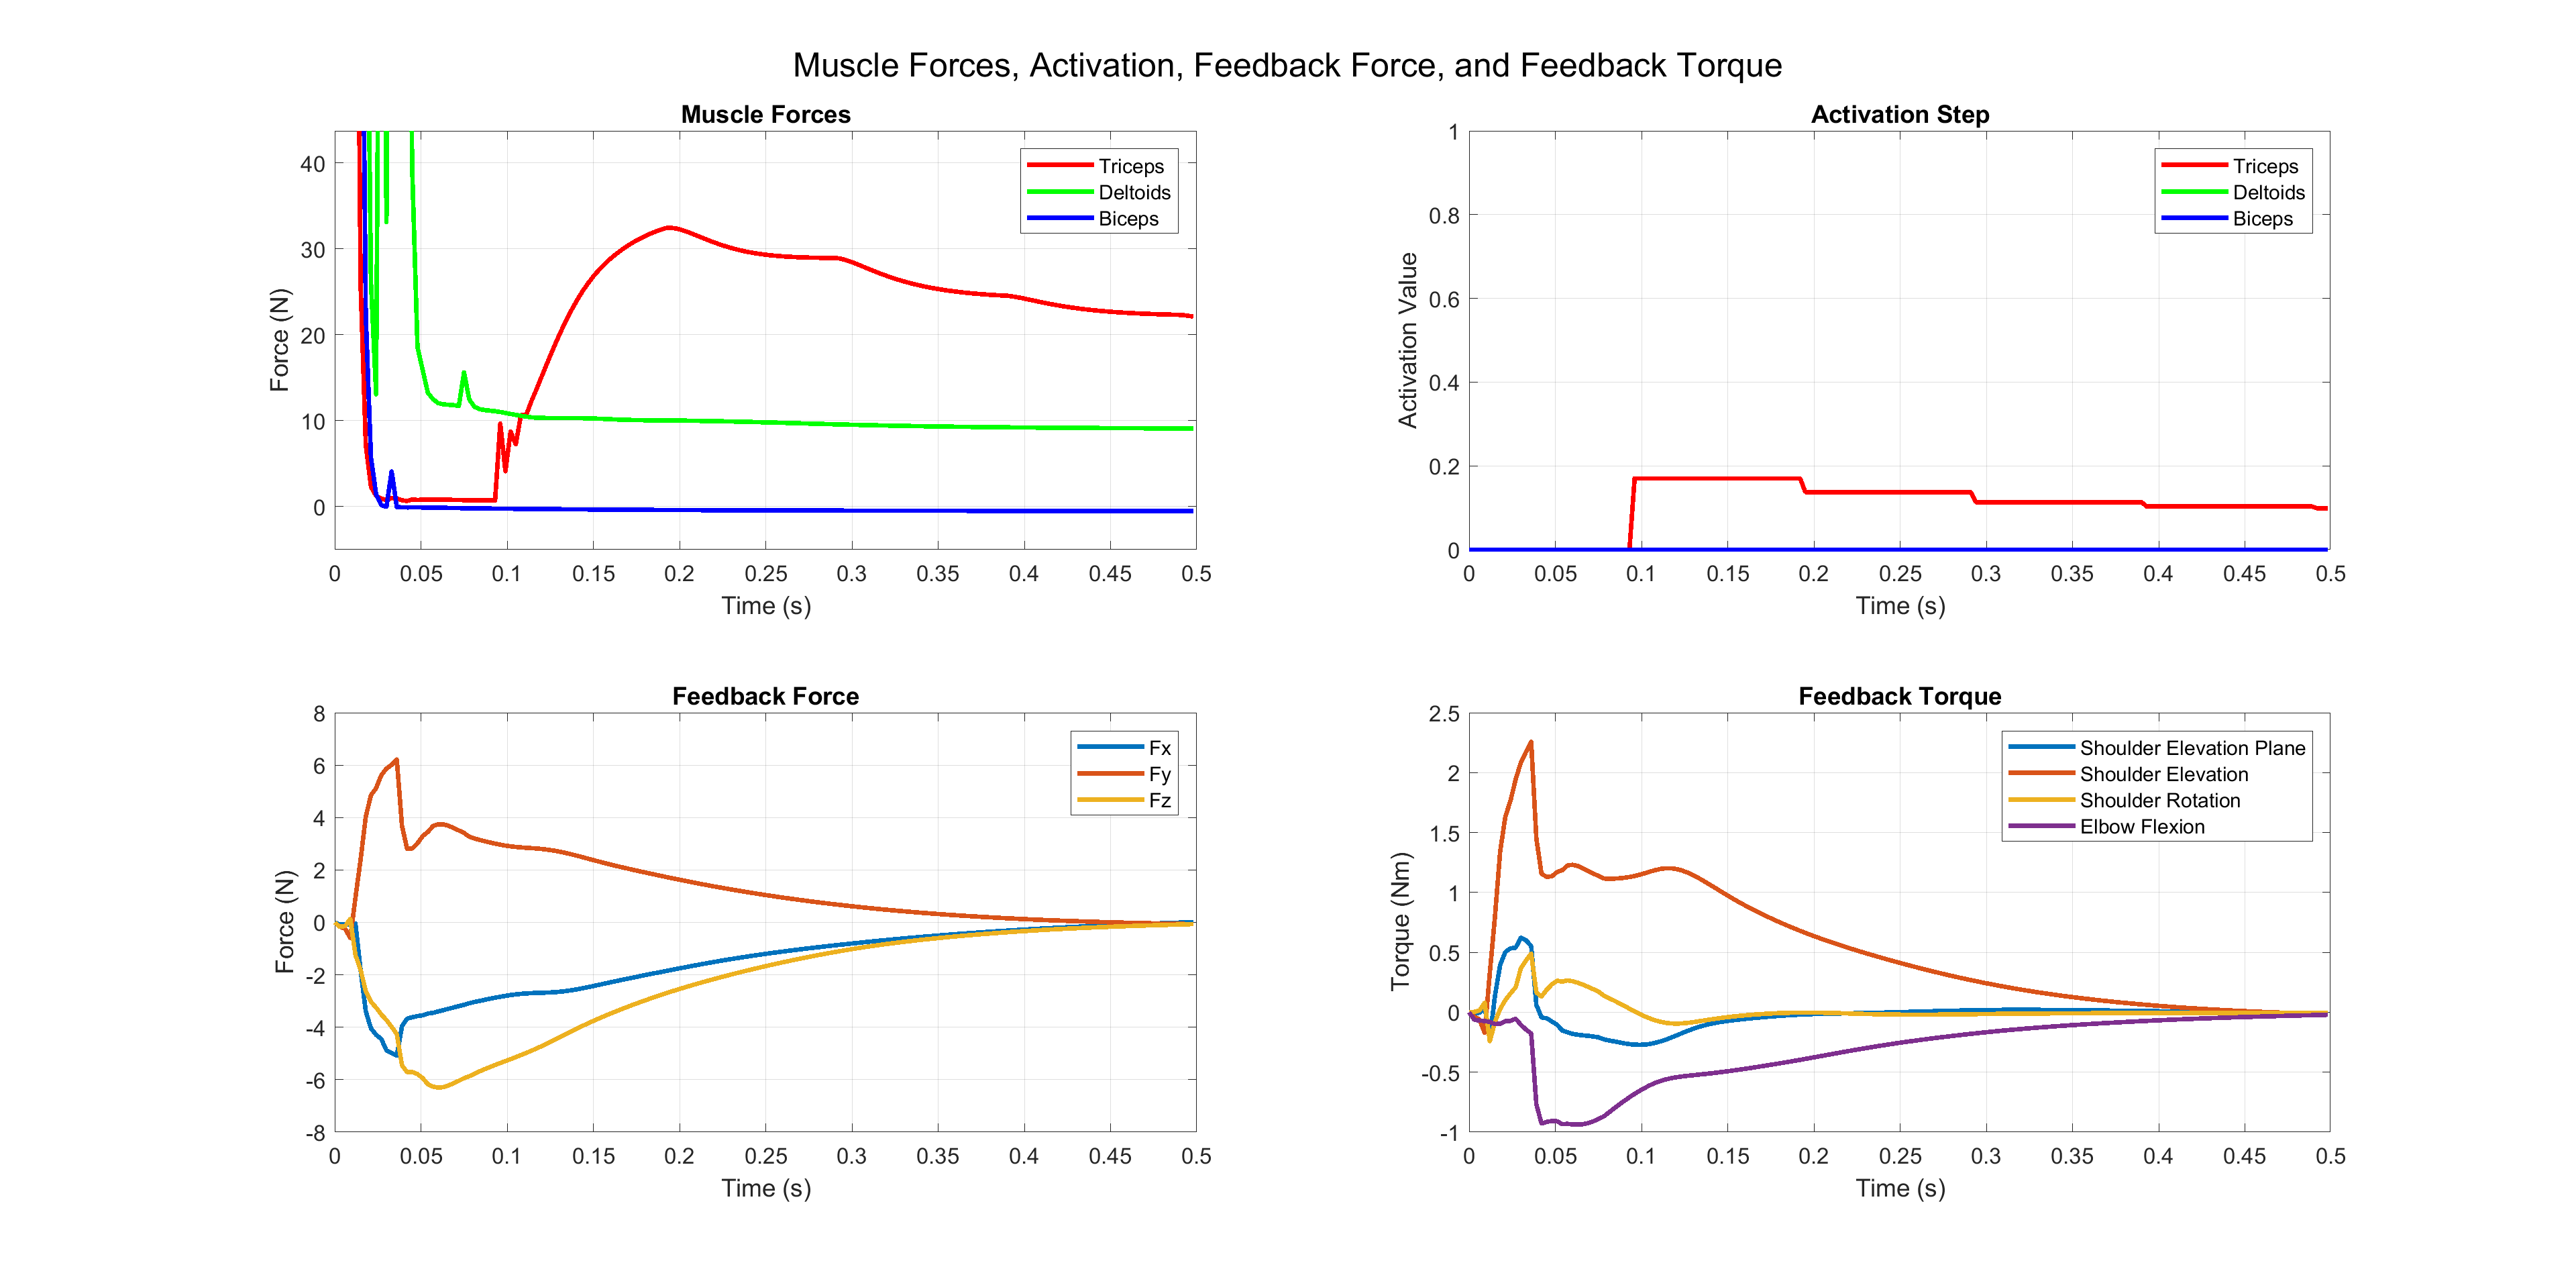
\includegraphics[width=1\textwidth]{Pictures/Controller/StaticControl.png} 
\caption{Static Control Example Muscle Forces, Activation Step, Feedback Force and Feedback Torque } % Optional caption
\label{fig:SC} % Optional label for referencing
\end{figure}

\begin{table}[h]
    \centering
    \scriptsize % Set font size
    \caption{Comparison between PI Values Results}
    \begin{tabularx}{\linewidth}{|X|X|X|}
        \hline
        \textbf{Controller} & \multicolumn{2}{c|}{\textbf{Target Position Error (m)}} \\
        \cline{2-3}
        & \textbf{Mean} & \textbf{Variance} \\
        \hline
        Kp = 100, Ki = 0 & [0.020 -0.026 0.003] & [0.060 0.238 0.025]$*10^{-3}$ \\
        \hline
        Kp = 100, Ki = 50  & [0.015 -0.021 0.003] & [0.046 0.160 0.024]$*10^{-3}$  \\
        \hline
        Kp = 300, Ki = 50 & [0.007 -0.012 0.002] & [0.012 0.041 0.013]$*10^{-3}$  \\
        \hline
        Kp = 300, Ki = 100 & [0.003 -0.012 -0.001] & [0.011 0.035 0.010]$*10^{-3}$  \\
        \hline
    \end{tabularx}
\end{table}

\begin{figure}[ht]
    \centering

    % Row 1, Column 1
    \begin{subfigure}[b]{0.45\textwidth}
        \centering
        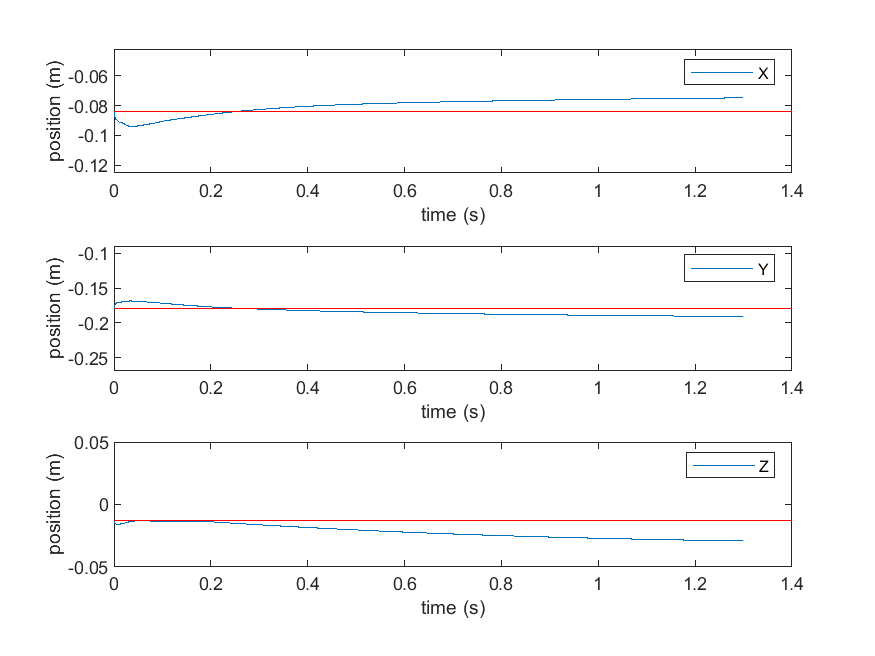
\includegraphics[width=\linewidth]{Pictures/Controller/Kp100Ki0/1.png}
        \caption{Position 1: Kp=100 Ki=0}
    \end{subfigure}%
    \hfill
    % Row 1, Column 2
    \begin{subfigure}[b]{0.45\textwidth}
        \centering
        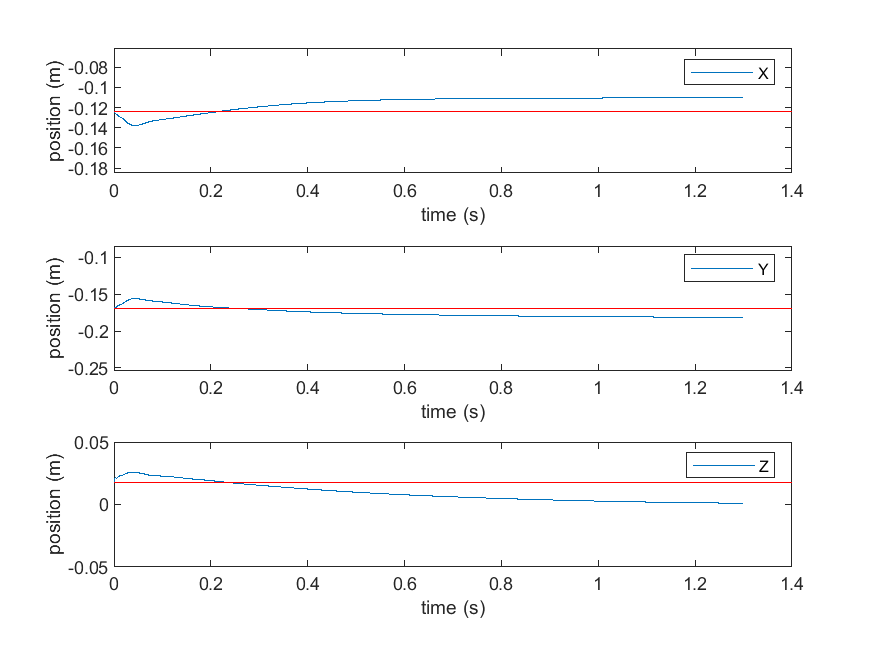
\includegraphics[width=\linewidth]{Pictures/Controller/Kp100Ki0/17.png}
        \caption{Position 2: Kp=100 Ki=0}
    \end{subfigure}

    \vspace{2pt} % Some vertical space between the rows

    % Row 2, Column 1
    \begin{subfigure}[b]{0.45\textwidth}
        \centering
        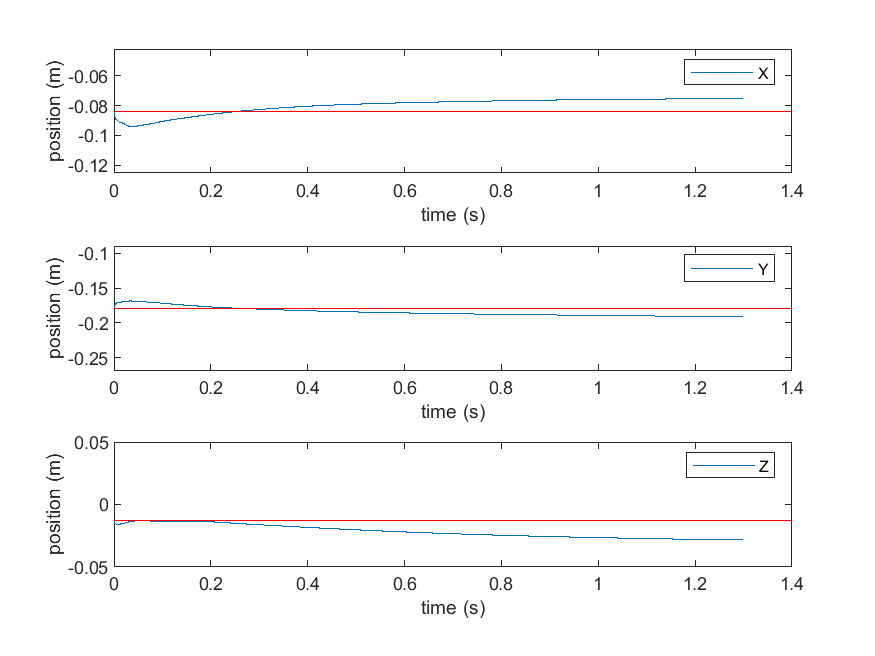
\includegraphics[width=\linewidth]{Pictures/Controller/Kp100Ki50/1.png}
        \caption{Position 1: Kp=100 Ki=50}
    \end{subfigure}%
    \hfill
    % Row 2, Column 2
    \begin{subfigure}[b]{0.45\textwidth}
        \centering
        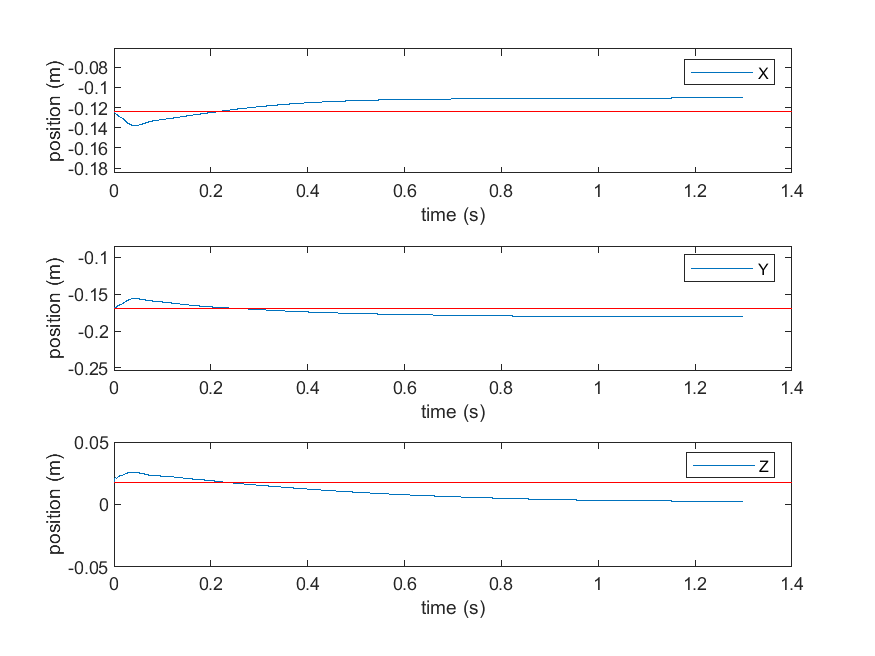
\includegraphics[width=\linewidth]{Pictures/Controller/Kp100Ki50/17.png}
        \caption{Position 2: Kp=100 Ki=50}
    \end{subfigure}

    \vspace{2pt} % Some vertical space between the rows

    % Row 3, Column 1
    \begin{subfigure}[b]{0.45\textwidth}
        \centering
        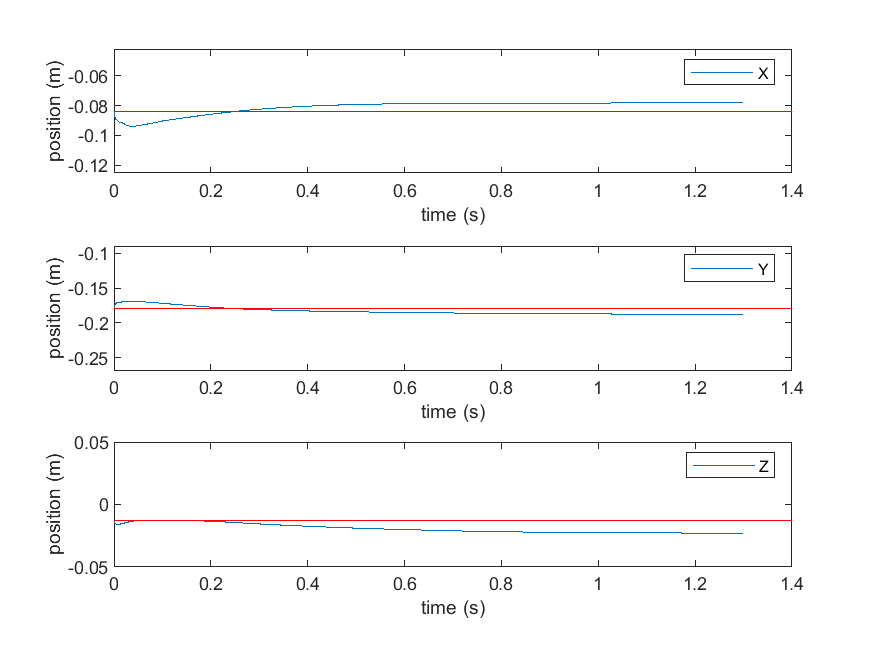
\includegraphics[width=\linewidth]{Pictures/Controller/Kp300Ki50/1.png}
        \caption{Position 1: Kp=300 Ki=50}
    \end{subfigure}%
    \hfill
    % Row 3, Column 2
    \begin{subfigure}[b]{0.45\textwidth}
        \centering
        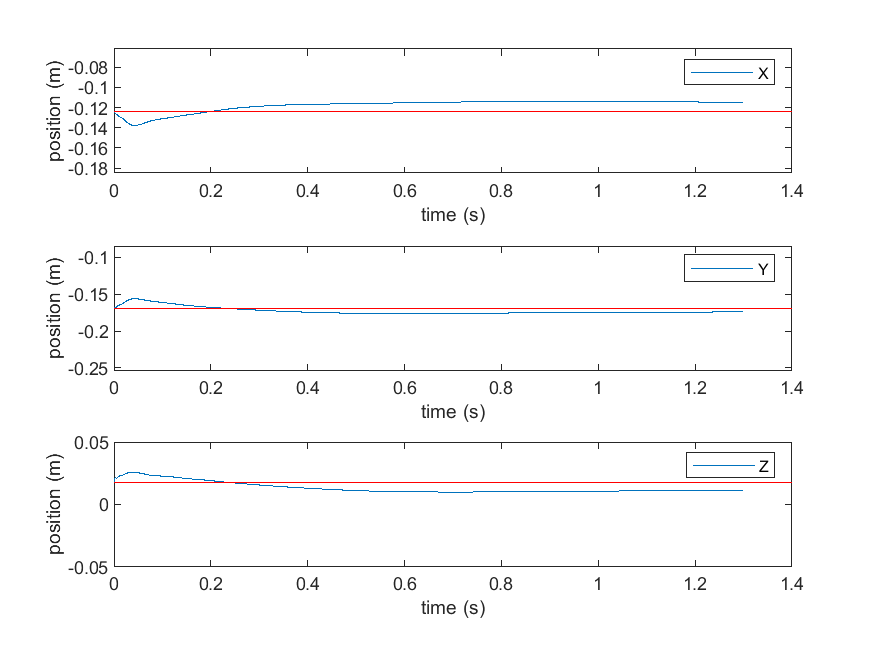
\includegraphics[width=\linewidth]{Pictures/Controller/Kp300Ki50/17.png}
        \caption{Position 2: Kp=300 Ki=50}
    \end{subfigure}

    \vspace{2pt} % Some vertical space between the rows

    % Row 4, Column 1
    \begin{subfigure}[b]{0.45\textwidth}
        \centering
        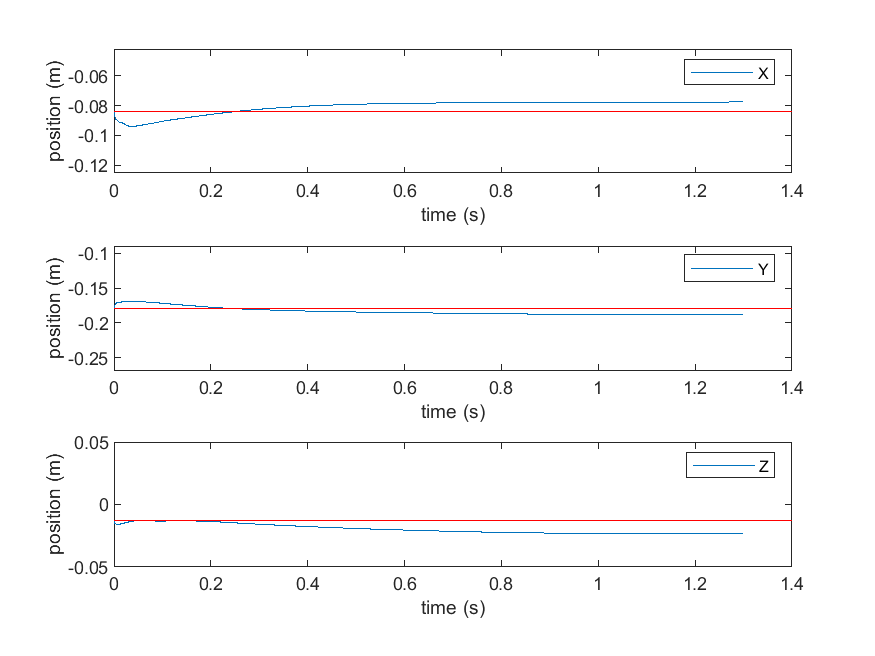
\includegraphics[width=\linewidth]{Pictures/Controller/Kp300Ki100/1.png}
        \caption{Position 1: Kp=300 Ki=100}
    \end{subfigure}%
    \hfill
    % Row 4, Column 2
    \begin{subfigure}[b]{0.45\textwidth}
        \centering
        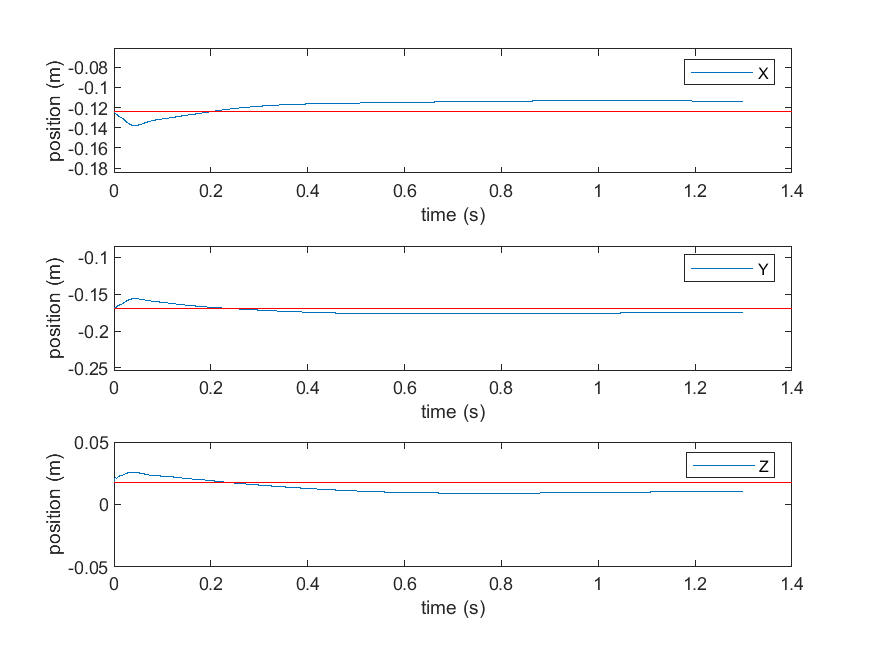
\includegraphics[width=\linewidth]{Pictures/Controller/Kp300Ki100/17.png}
        \caption{Position 2: Kp=300 Ki=100}
    \end{subfigure}

    \caption{Static Controller Different PI values for Tuning}
    \label{fig:staticPItuning}
\end{figure}


\newpage
\begin{landscape} % Start landscape page
  \begin{figure}[h!]
    \centering
    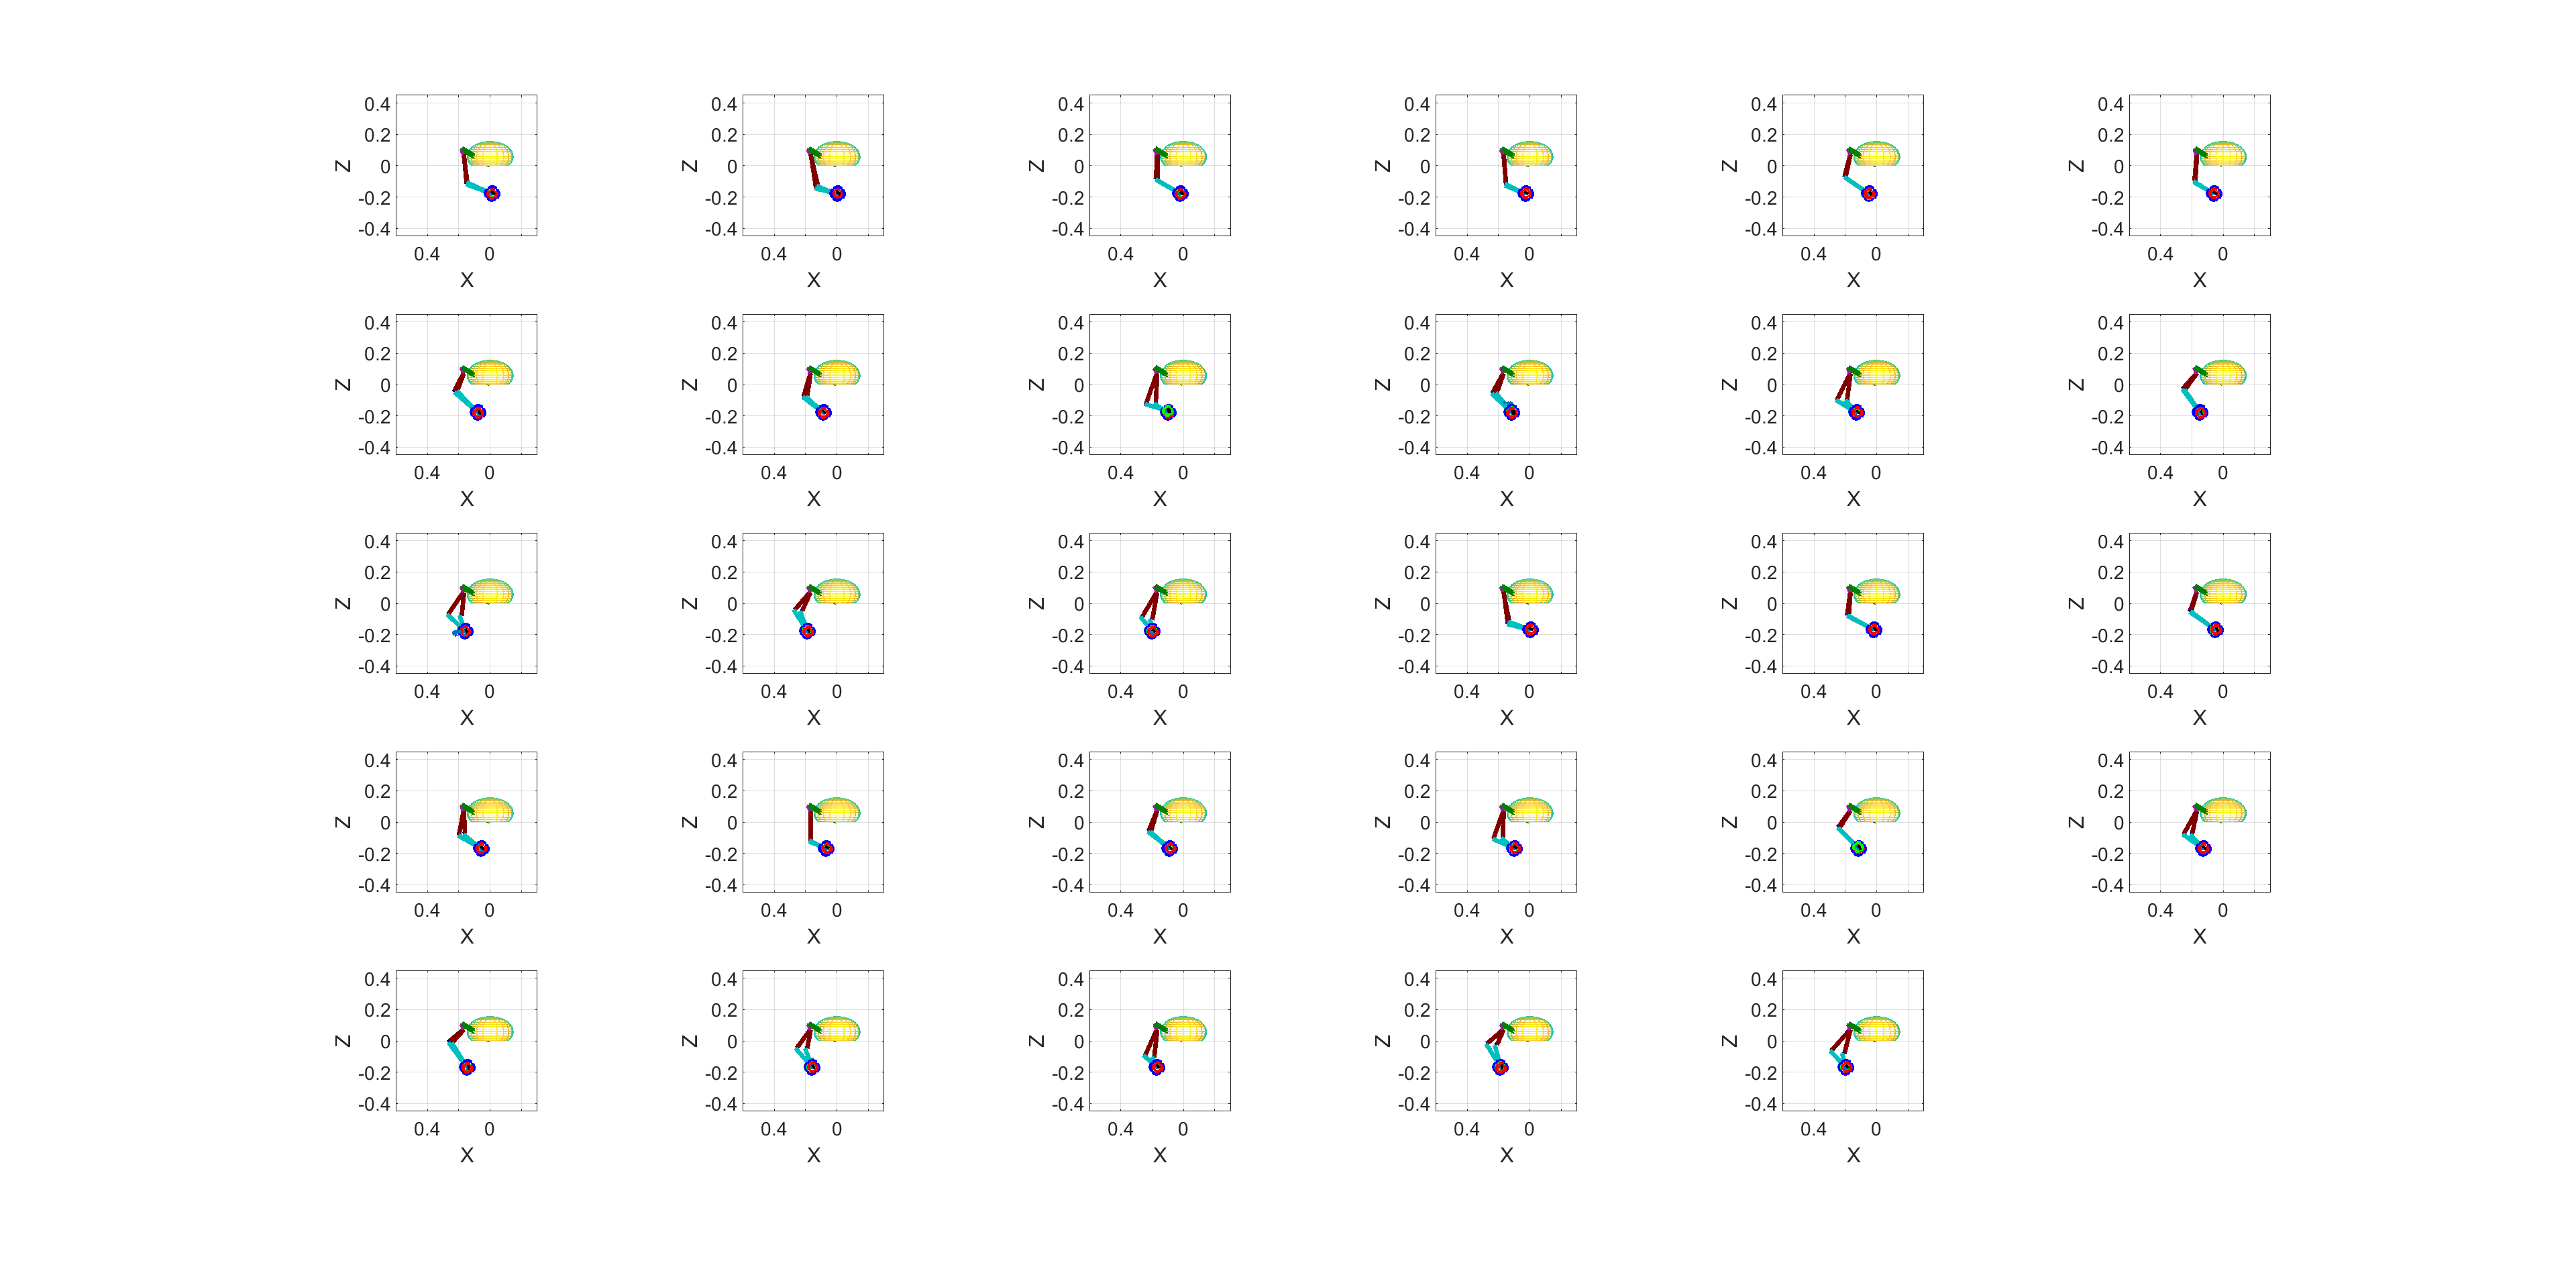
\includegraphics[width=1.9\textwidth]{Pictures/Controller/Static29positions.png} % Replace "filename.jpg" with the name of your image file
    \caption{Desired Targets in Static Control} % Optional caption
    \label{29statics}

  \end{figure}
\end{landscape} % End landscape page




\subsection{Path Following Quasi-Static Controller}
The path following quasi-static controller successfully found a path for each of the 29 points (see Figure \ref{fig:pqsc}). The table below presents the mean target position error and the variance. It can be seen that even though some of the intermediate points were not reached perfectly the target position is reached with a maximum error of 0.012 in the y coordinate. 

Figure \ref{fig:pfqscwp} shows 3 examples of the 29 positions where it can be seen the progression of the wrist position over time. It can be seen that in some cases there exists some oscillations. This could be improved by the addition of a derivative gain in the controller. 


\begin{table}[h]
    \centering
    \scriptsize % Set font size
    \caption{Comparison between PI Values Results}
    \begin{tabularx}{\linewidth}{|X|X|X|}
        \hline
        \textbf{Controller} & \multicolumn{2}{c|}{\textbf{Target Position Error (m)}} \\
        \cline{2-3}
        & \textbf{Mean} & \textbf{Variance} \\
        \hline
        Quasi-Static & [0.003 -0.012 -0.001] & [0.363 0.045 0.019]$*10^{-3}$ \\
        \hline
    \end{tabularx}
\end{table}

\begin{figure}[ht]
    \centering

    % Row 1, Column 1
    \begin{subfigure}[b]{0.45\textwidth}
        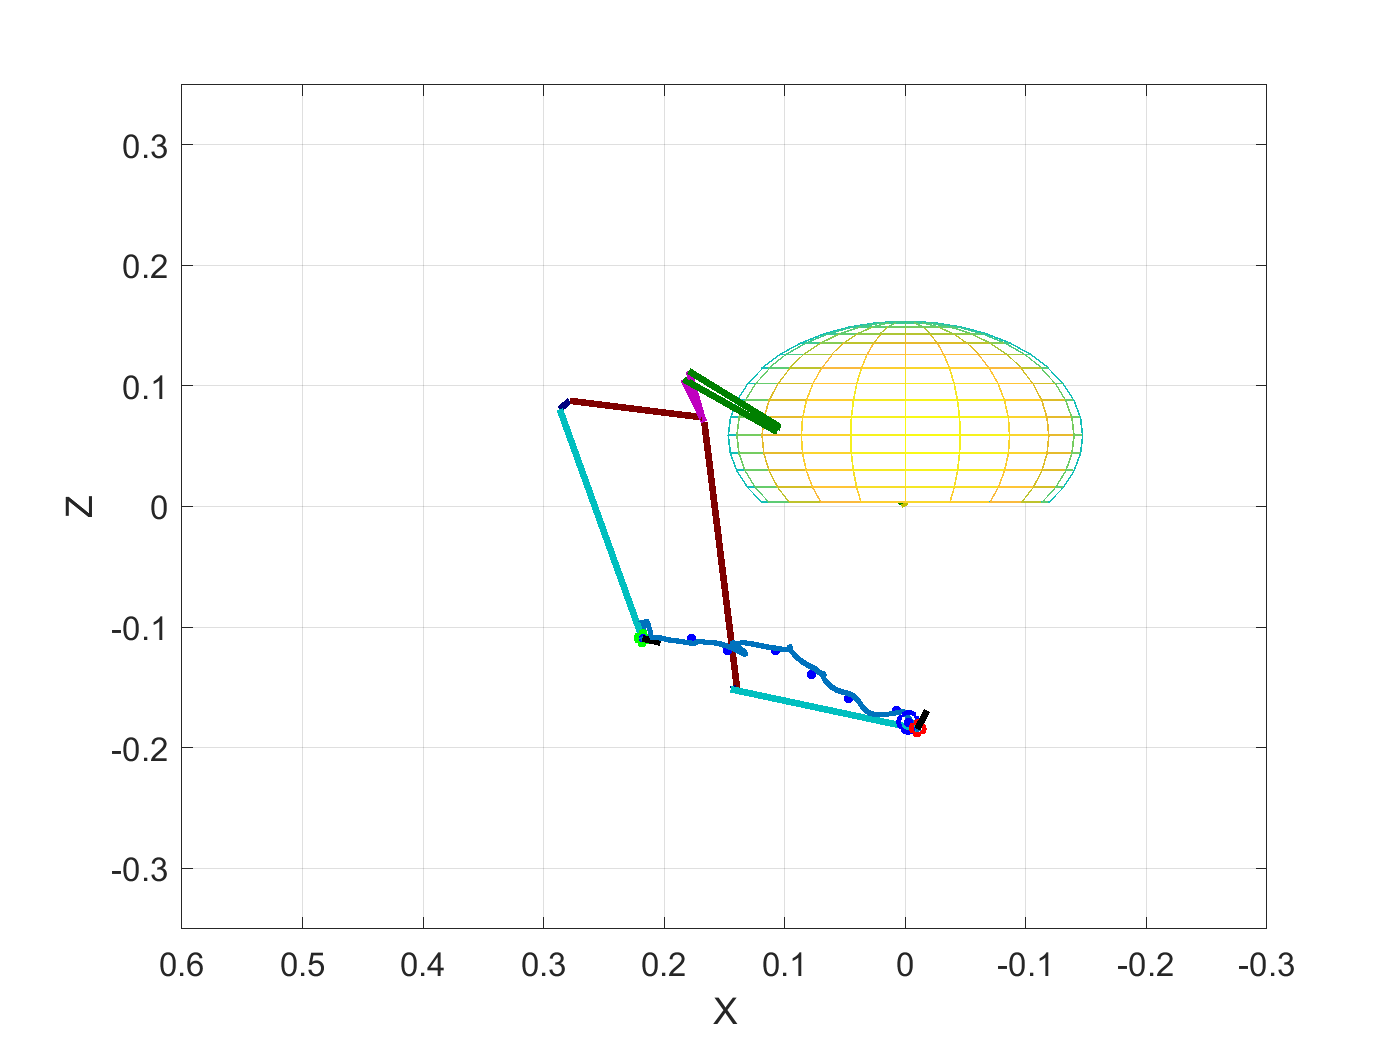
\includegraphics[width=0.8\linewidth]{Pictures/Controller/QSC/2_wp.png}
        \caption{Position 1: Wrist Position Plot 3D}
    \end{subfigure}%
    \hfill
    % Row 1, Column 2
    \begin{subfigure}[b]{0.45\textwidth}
        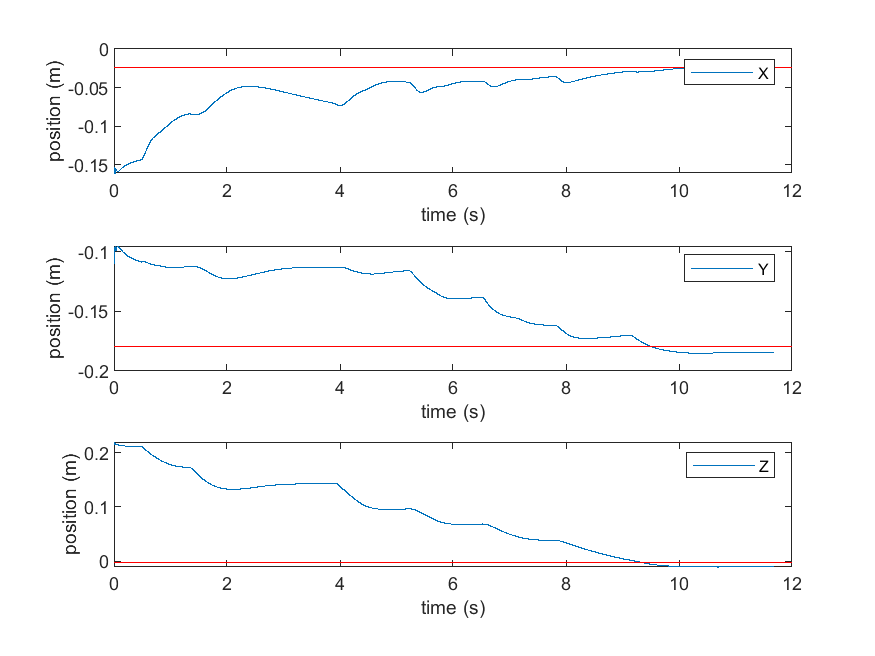
\includegraphics[width=0.8\linewidth]{Pictures/Controller/QSC/2.png}
        \caption{Position 1: Wrist Position Plot 2D}
    \end{subfigure}

    \vspace{2pt} % Some vertical space between the rows

    % Row 2, Column 1
    \begin{subfigure}[b]{0.45\textwidth}
        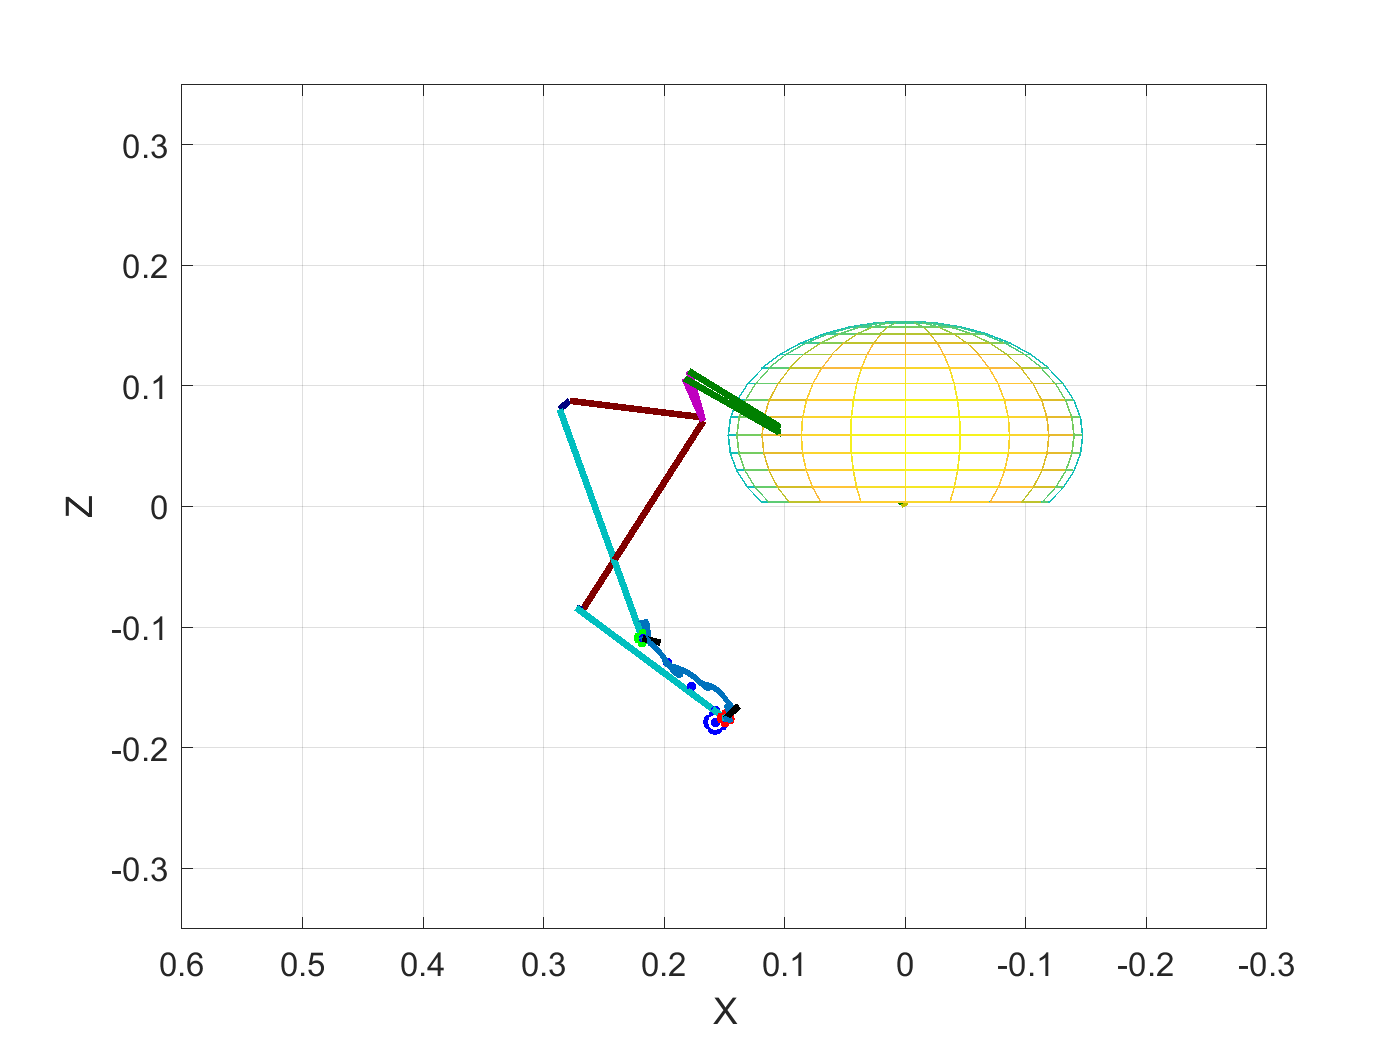
\includegraphics[width=0.8\linewidth]{Pictures/Controller/QSC/13_wp.png}
        \caption{Position 2: Wrist Position Plot 3D}
    \end{subfigure}%
    \hfill
    % Row 2, Column 2
    \begin{subfigure}[b]{0.45\textwidth}
        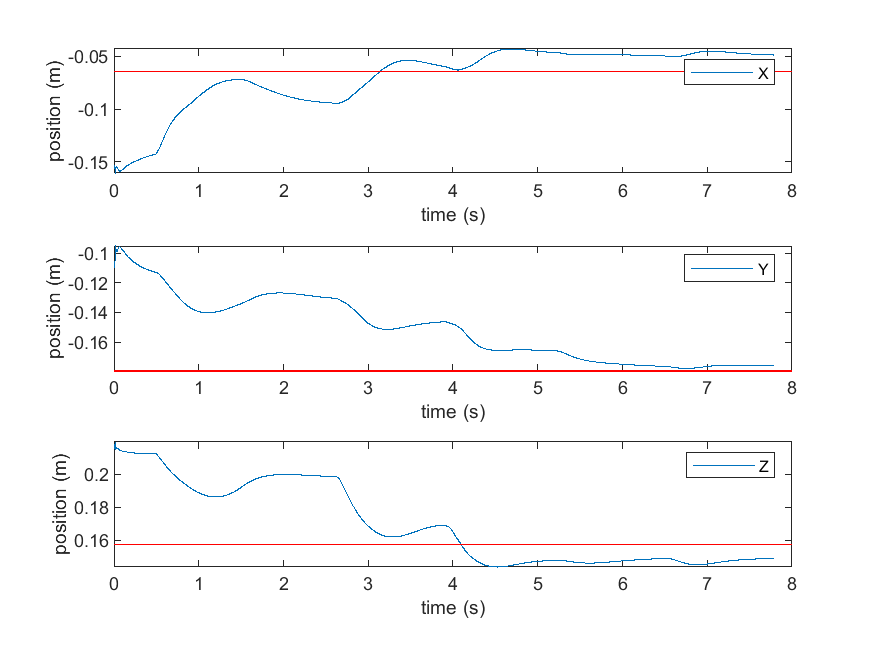
\includegraphics[width=0.8\linewidth]{Pictures/Controller/QSC/13.png}
        \caption{Position 2: Wrist Position Plot 2D}
    \end{subfigure}

    \vspace{2pt} % Some vertical space between the rows

    % Row 3, Column 1
    \begin{subfigure}[b]{0.45\textwidth}
        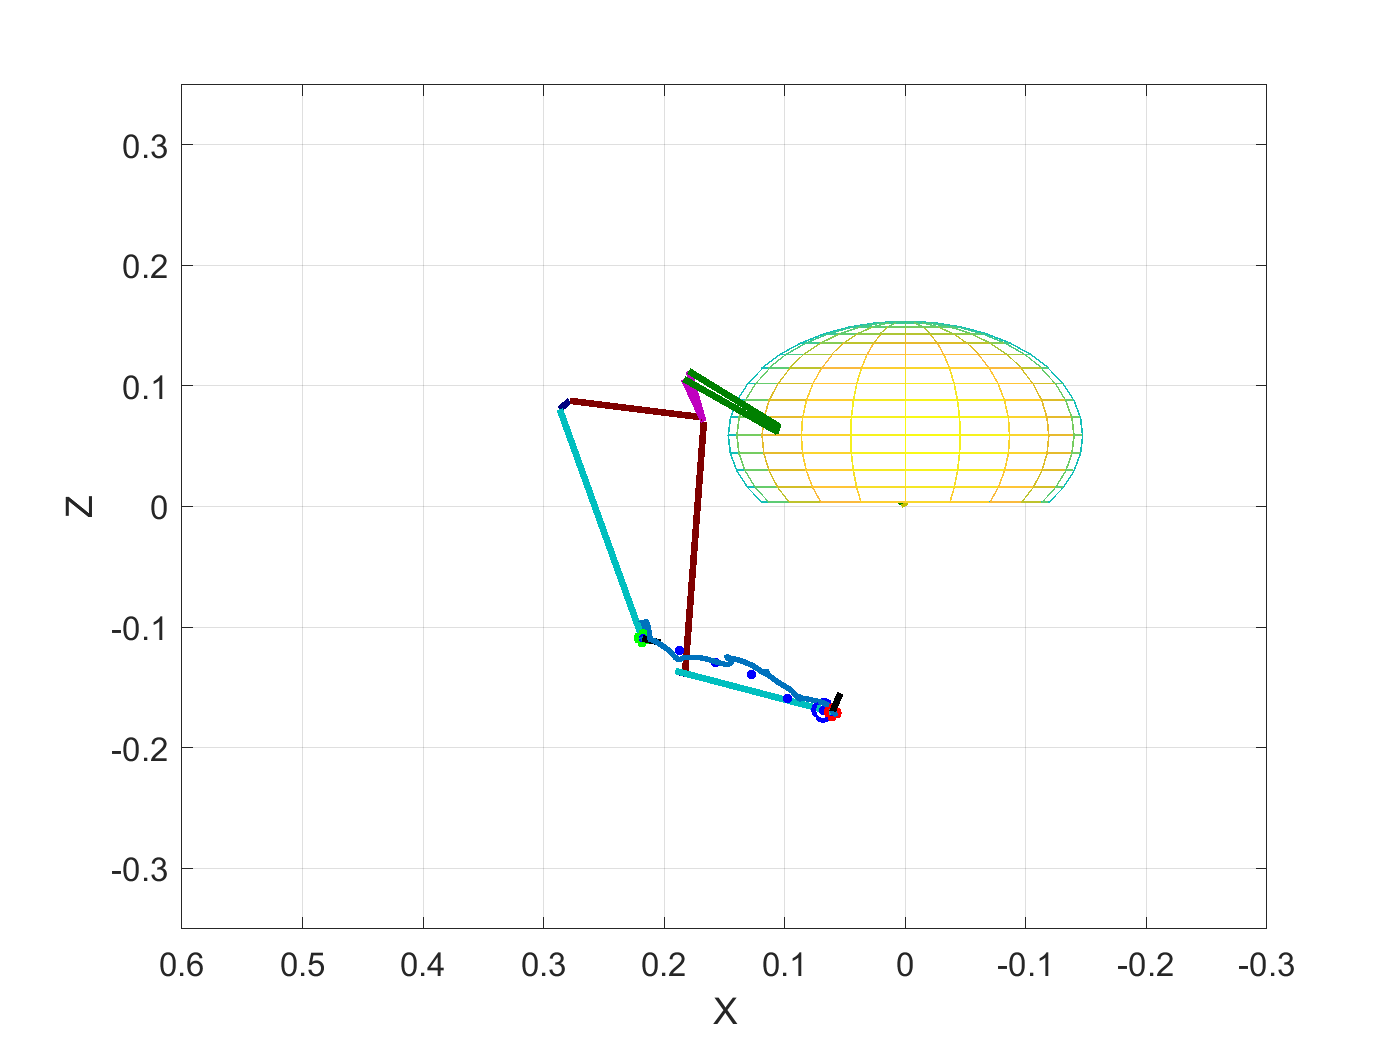
\includegraphics[width=0.8\linewidth]{Pictures/Controller/QSC/20_wp.png}
        \caption{Position 3: Wrist Position Plot 2D}
    \end{subfigure}%
    \hfill
    % Row 3, Column 2
    \begin{subfigure}[b]{0.45\textwidth}
        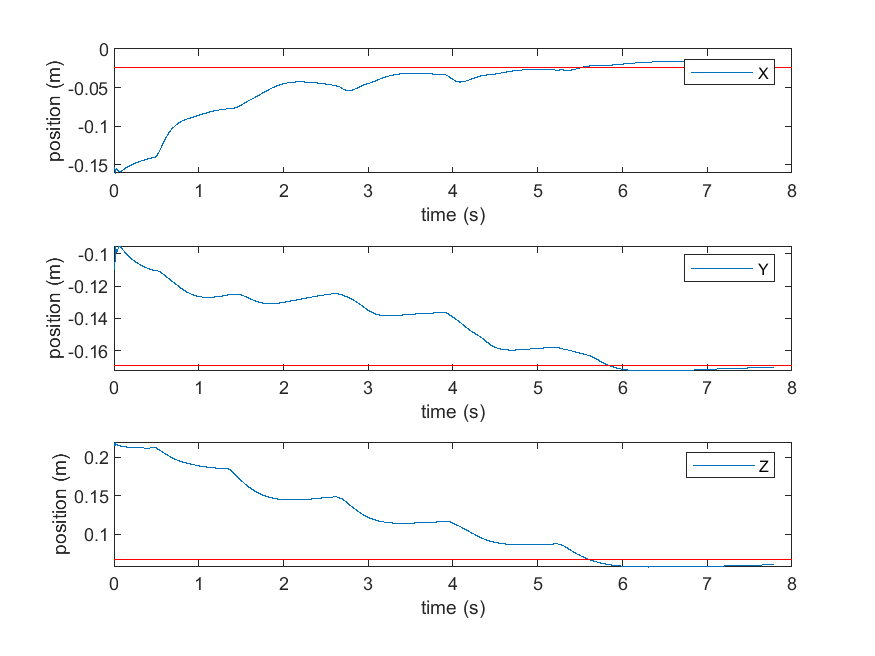
\includegraphics[width=0.8\linewidth]{Pictures/Controller/QSC/20.png}
        \caption{Position 3: Wrist Position Plot 2D}
    \end{subfigure}

    \caption{Path Following Quasi-Static Controller}
    \label{fig:pfqscwp}
\end{figure}

\newpage
\begin{landscape} % Start landscape page
  \begin{figure}[h!]
    \centering
    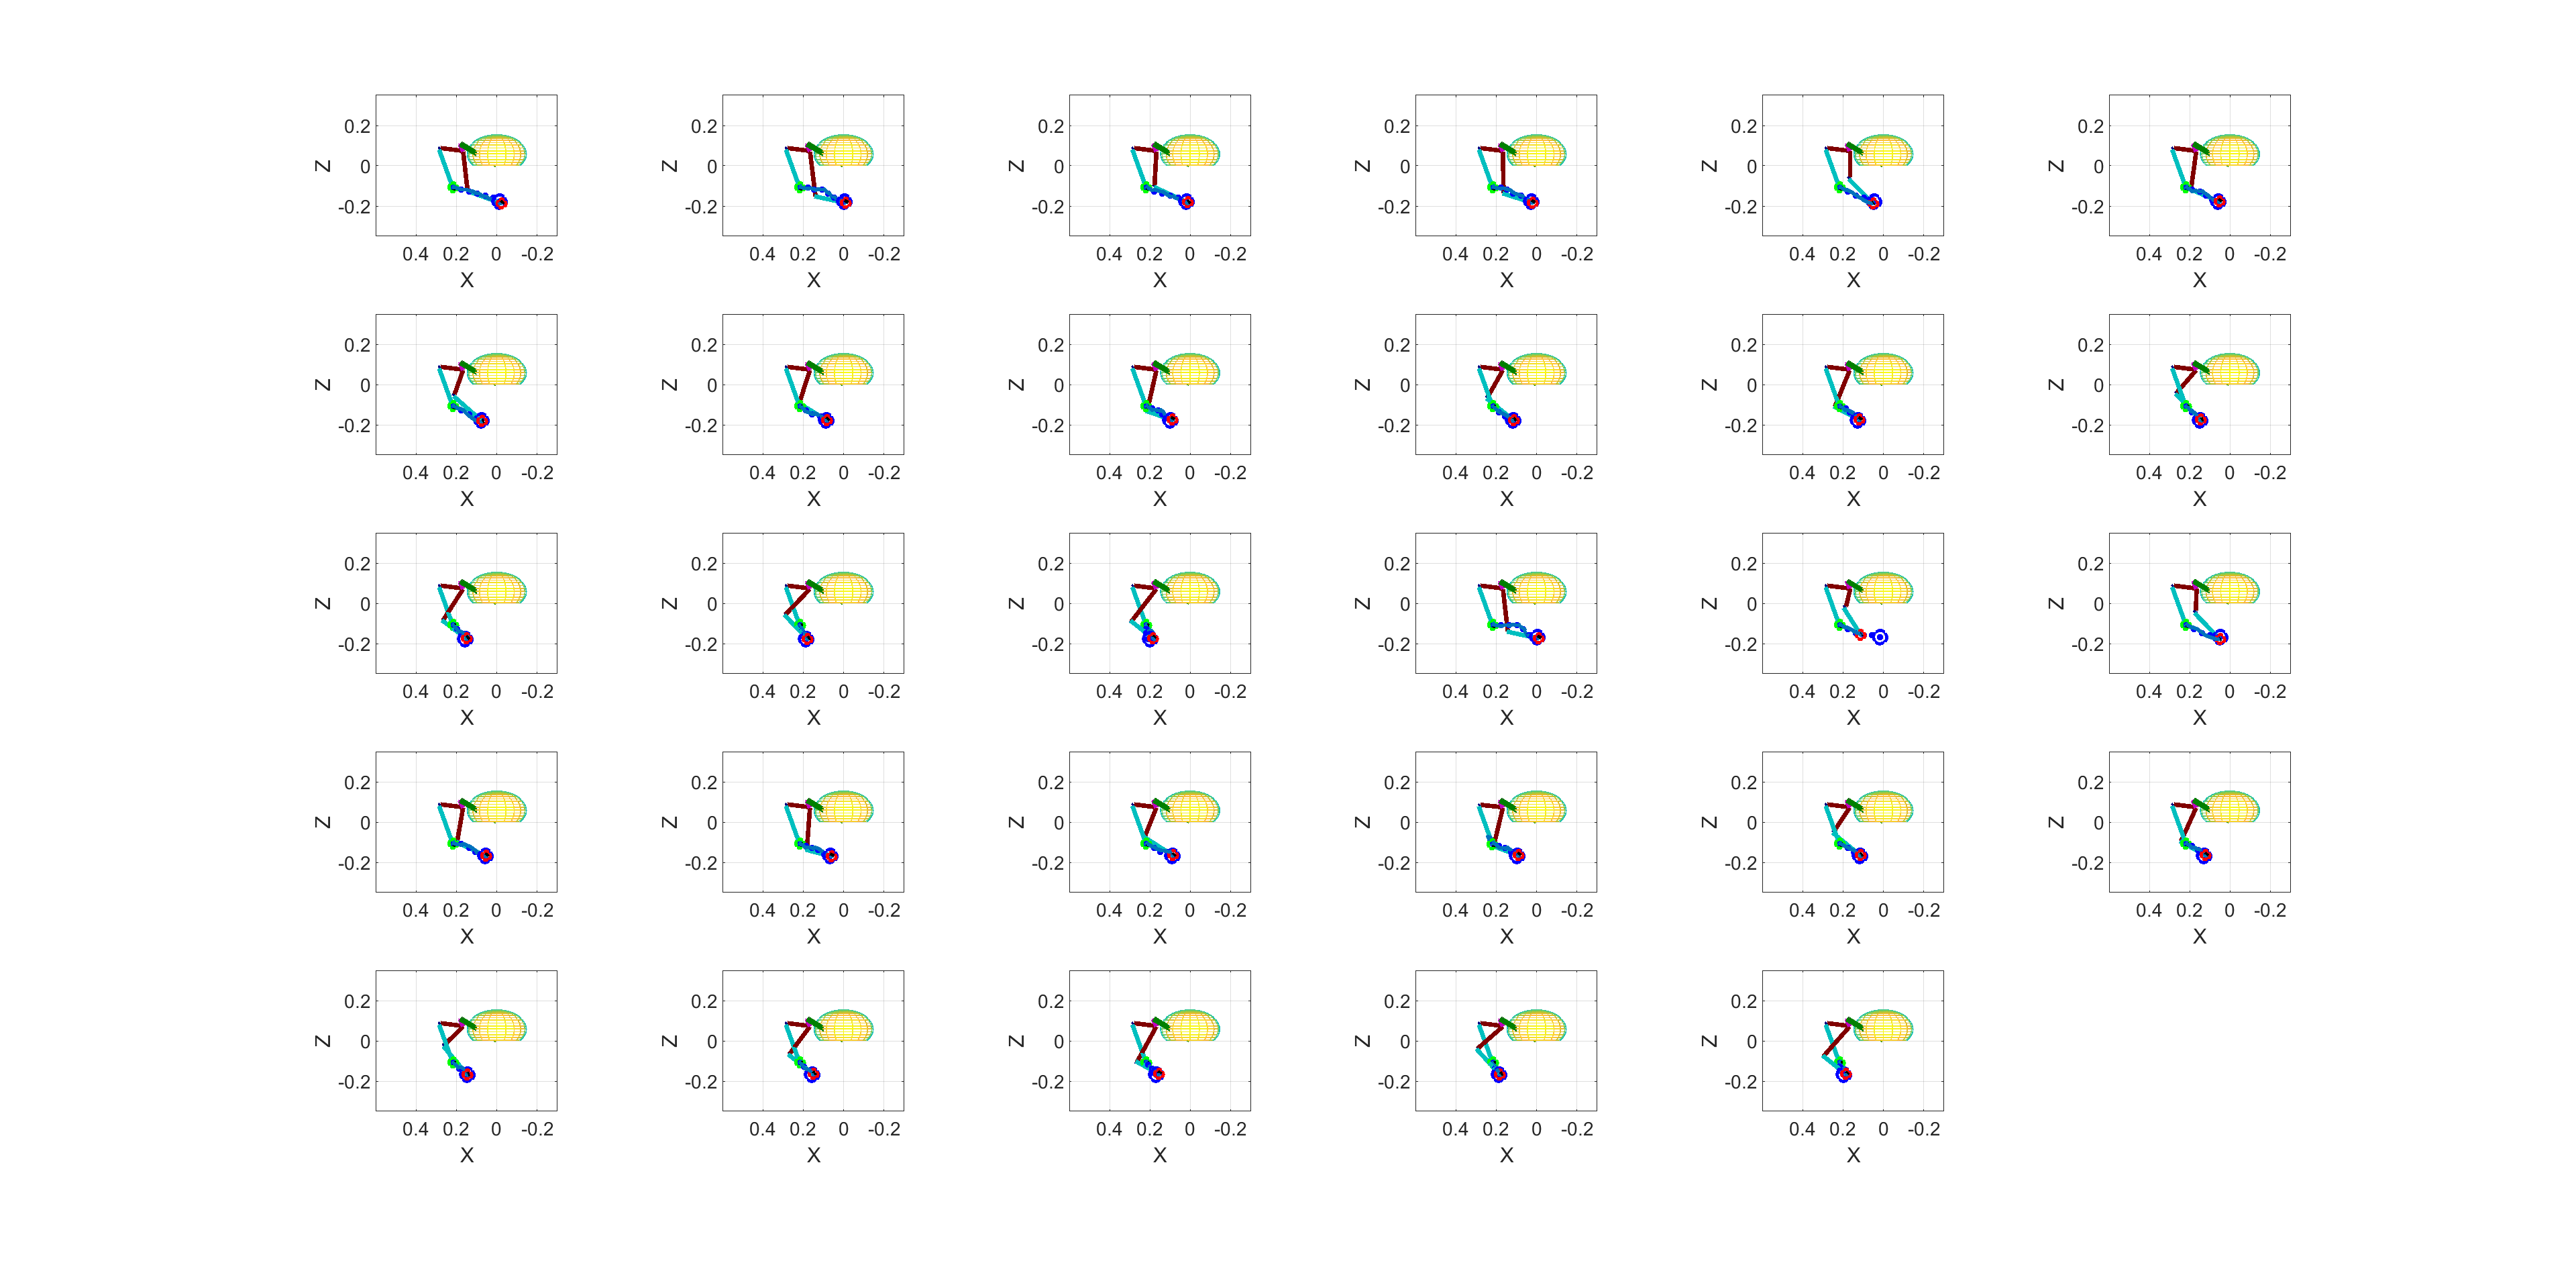
\includegraphics[width=1.7\textwidth]{Pictures/Results/Controller/QSC29positions.png}
    \caption{Desired Targets in Path-Following Quasi-Static Control} 
    \label{fig:pqsc}
  \end{figure}
\end{landscape} % End landscape page

\subsection{EMG-Influenced Control}

This section comprises two parts. The first pertains to objective number 2, as illustrated in Figure \ref{fig:bdd}, emphasizing the inclusion of the stroke parameter based on the design criteria. The latter part focuses on objective 3, integrating the FES controller to counterbalance the stroke's repercussions, thereby facilitating patients in accomplishing the reaching movement.

\subsubsection{Emulating Biceps Over-Activity}
Figure \ref{fig: comparisonmuscleactivity} illustrates the over-activity effect of the stroke factor on the biceps' muscle activity (index = 2), leading to its over-activation. Additionally, the compensatory behavior of other muscles is evident as they respond to this heightened activity.

\begin{figure}[ht]
    \centering
    % Row 1, Column 1
    \begin{subfigure}[b]{0.45\textwidth}
        \centering
        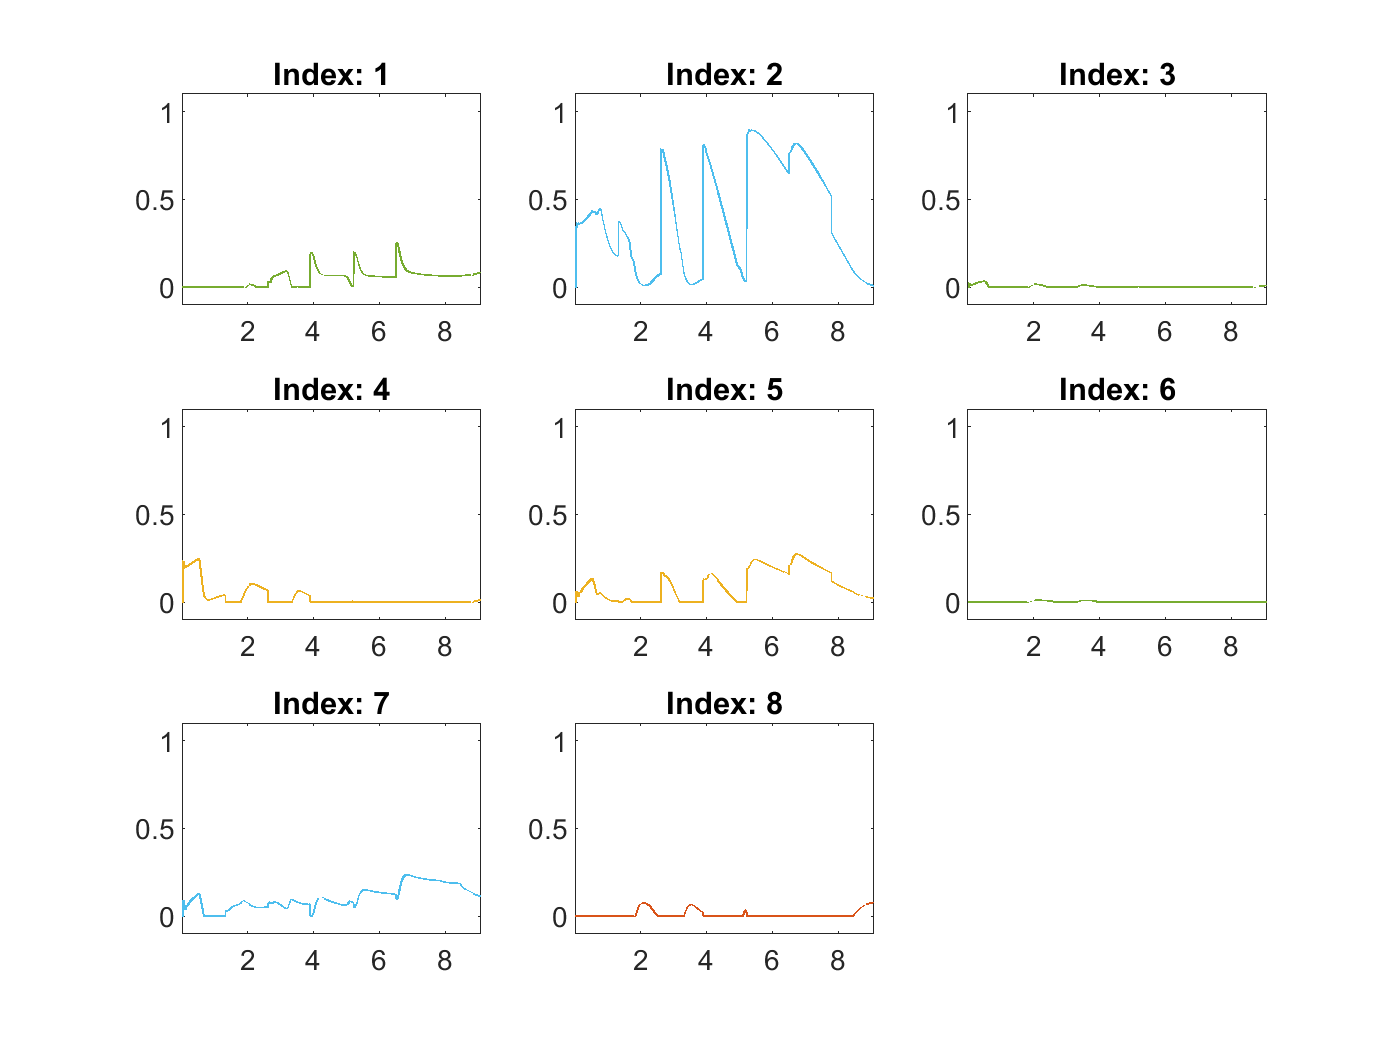
\includegraphics[width=\linewidth]{Pictures/Results/Controller/Healthy_NA.png}
        \caption{Non-Stroke Muscle Activity}
    \end{subfigure}%
    \hfill
    % Row 1, Column 2
    \begin{subfigure}[b]{0.45\textwidth}
        \centering
        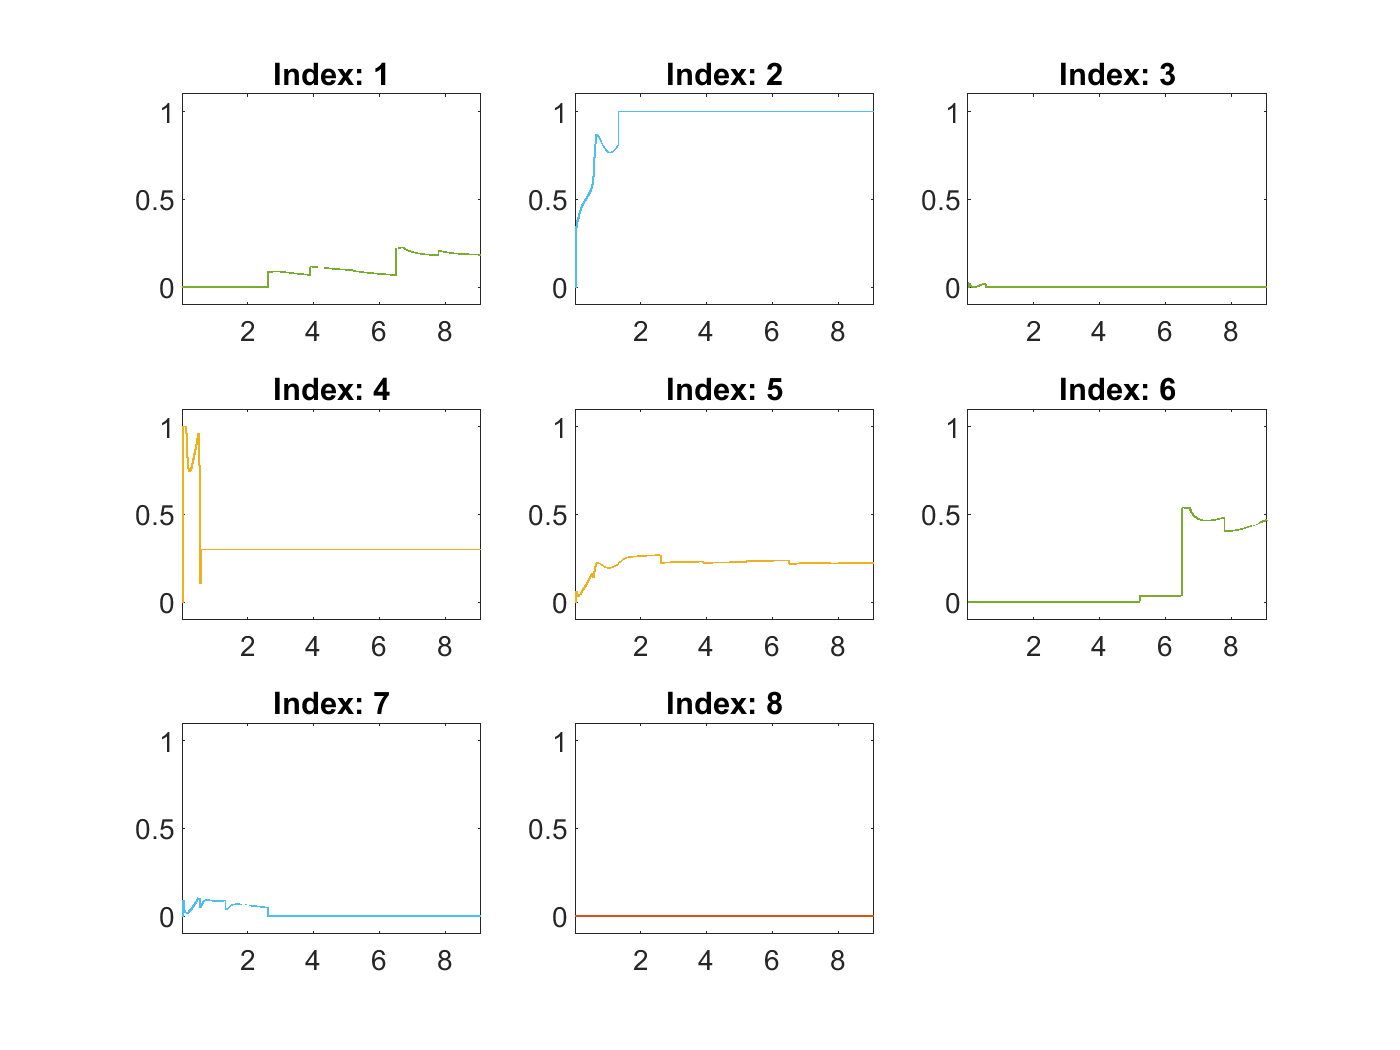
\includegraphics[width=\linewidth]{Pictures/Results/Controller/StrokeWithouControl_NA.png}
        \caption{Stroke = 7 Muscle Activity}
    \end{subfigure}

    \vspace{2pt} % Some vertical space between the rows

    \begin{subfigure}[b]{0.45\textwidth}
        \centering
        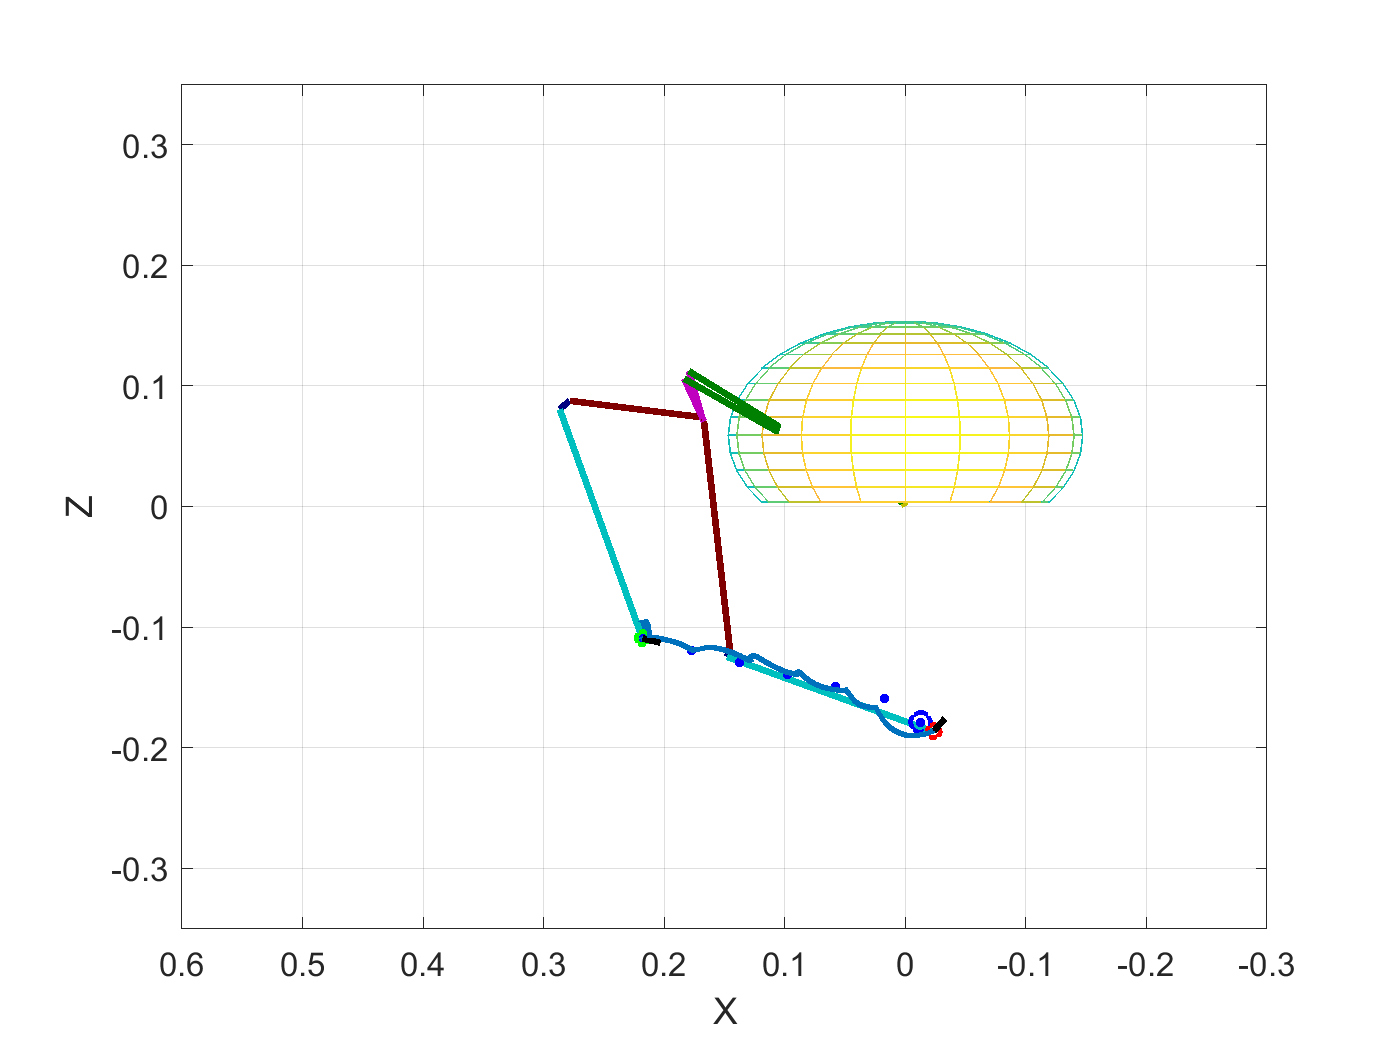
\includegraphics[width=\linewidth]{Pictures/Results/Controller/Healthy_WP.png}
        \caption{Non-Stroke Wrist Position 3D}
    \end{subfigure}%
    \hfill
    % Row 1, Column 2
    \begin{subfigure}[b]{0.45\textwidth}
        \centering
        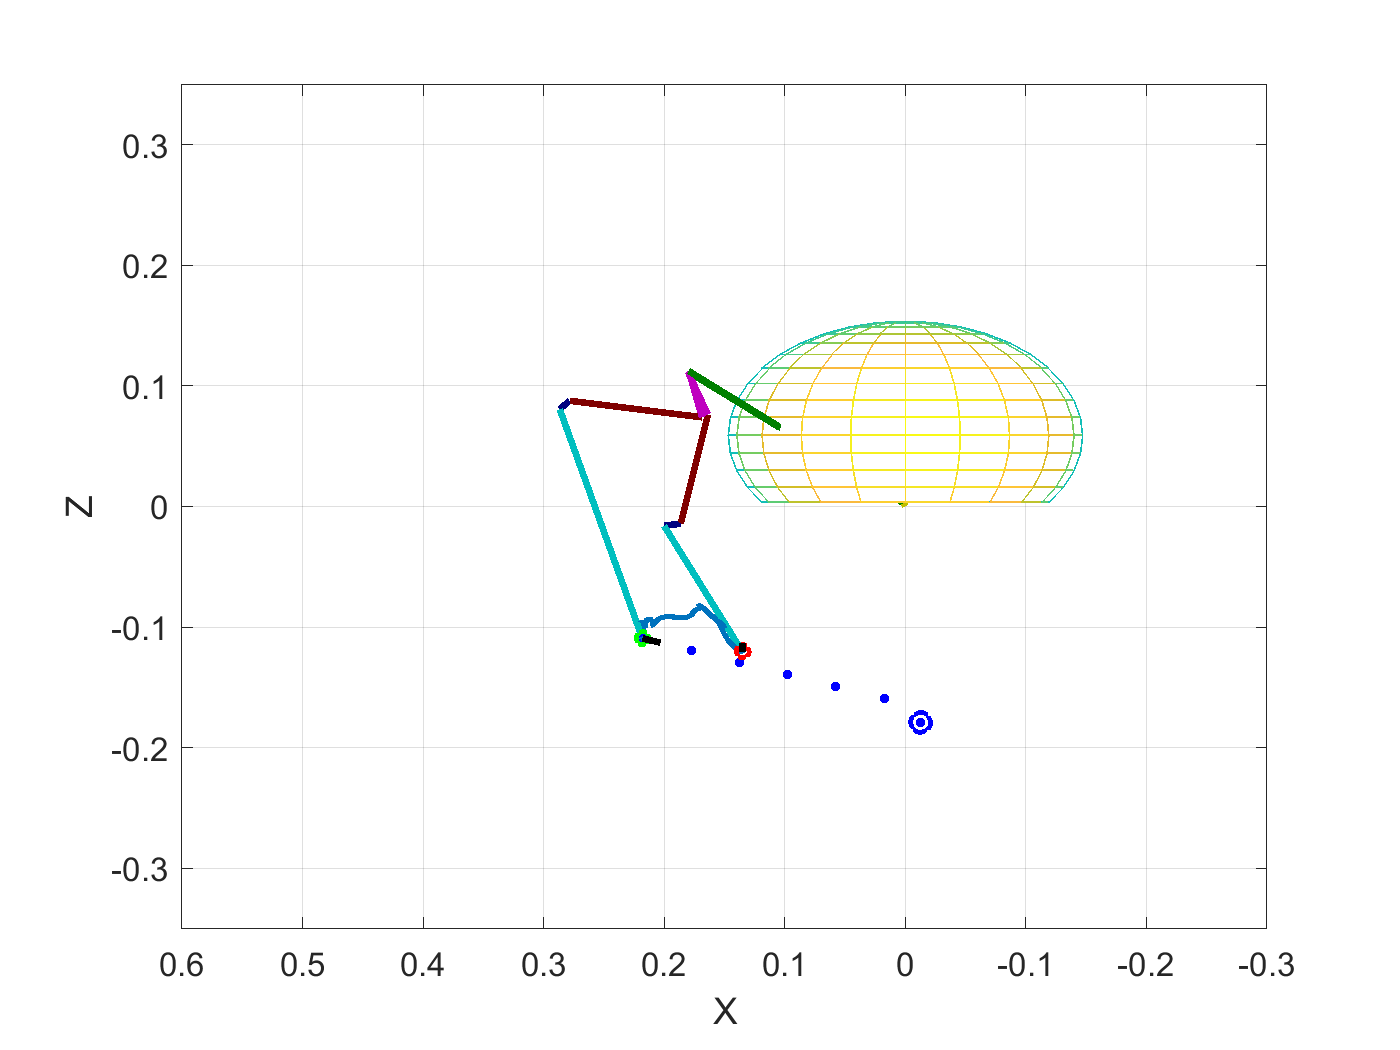
\includegraphics[width=\linewidth]{Pictures/Results/Controller/StrokeWithouControl_WP.png}
        \caption{Stroke=7 Wrist Position 3D}
    \end{subfigure}
        
    \caption{Comparison of Muscle Activity and Wrist Position 3D}
    \label{fig: comparisonmuscleactivity}
\end{figure}

\subsubsection{FES EMG-Influenced Control for Triceps}


\begin{table}[h]
    \centering
    \scriptsize % Set font size
    \caption{Comparison between Stroke Values}
    \begin{tabularx}{\linewidth}{|X|X|X|}
        \hline
        \textbf{Controller} & \multicolumn{2}{c|}{\textbf{Target Position Error (m)}} \\
        \cline{2-3}
        & \textbf{Mean} & \textbf{Variance} \\
        \hline
        Stroke = 3 & [0.009 -0.030 0.004] & [0.059 0.024 0.103]$*10^{-3}$ \\
        \hline
        Stroke = 7  & [0.007 -0.029 -0.003] & [0.048 0.015 0.163]$*10^{-3}$  \\
        \hline
        Stroke = 10 & [0.006 -0.028 -0.005] & [0.046 0.018 0.189]$*10^{-3}$  \\
        \hline
        Non-Stroke & [0.003 -0.012 -0.001] & [0.363 0.045 0.019]$*10^{-3}$  \\
        \hline
    \end{tabularx}
\end{table}


\begin{figure}[ht]
    \centering
    % Row 1, Column 1
    \begin{subfigure}[b]{0.45\textwidth}
        \centering
        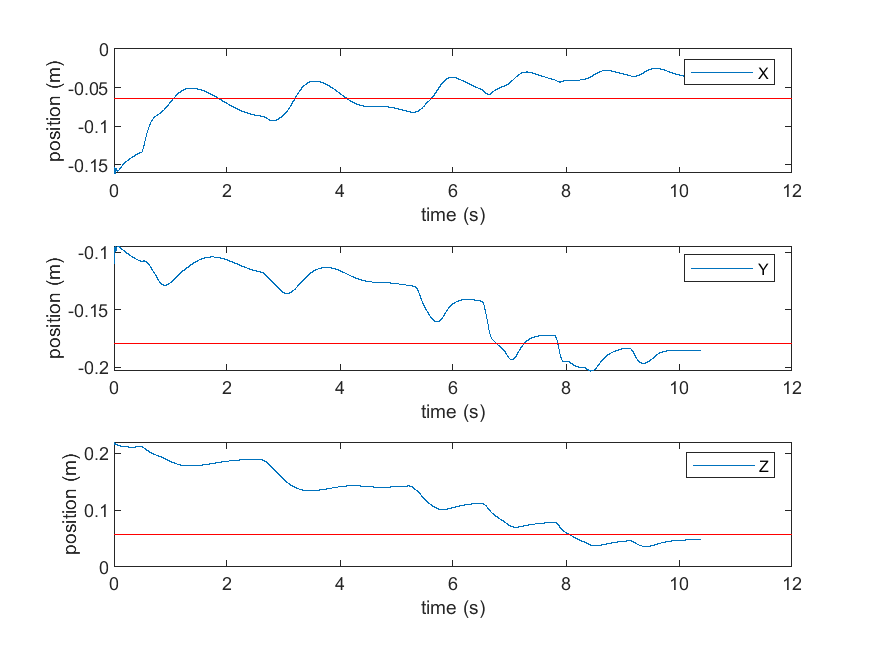
\includegraphics[width=\linewidth]{Pictures/Results/Controller/Stroke3/6.png}
        \caption{Example 1. Stroke=3.}
    \end{subfigure}%
    \hfill
    % Row 1, Column 2
    \begin{subfigure}[b]{0.45\textwidth}
        \centering
        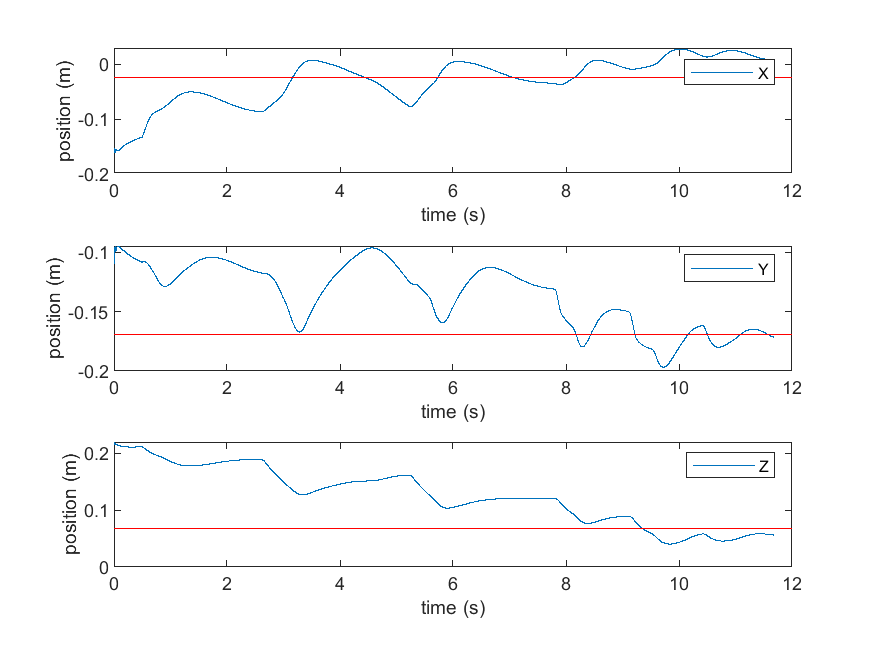
\includegraphics[width=\linewidth]{Pictures/Results/Controller/Stroke3/20.png}
        \caption{Example 2. Stroke=3.}
    \end{subfigure}
    
    \vspace{2pt} % Some vertical space between the rows

        \begin{subfigure}[b]{0.45\textwidth}
        \centering
        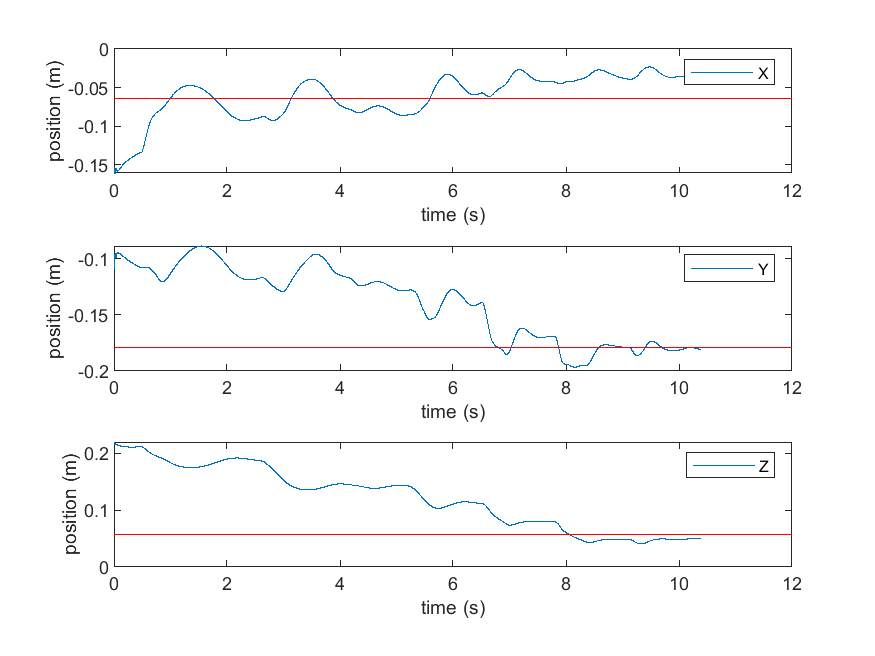
\includegraphics[width=\linewidth]{Pictures/Results/Controller/Stroke7/6.png}
        \caption{Example 1. Stroke=7.}
    \end{subfigure}%
    \hfill
    % Row 1, Column 2
    \begin{subfigure}[b]{0.45\textwidth}
        \centering
        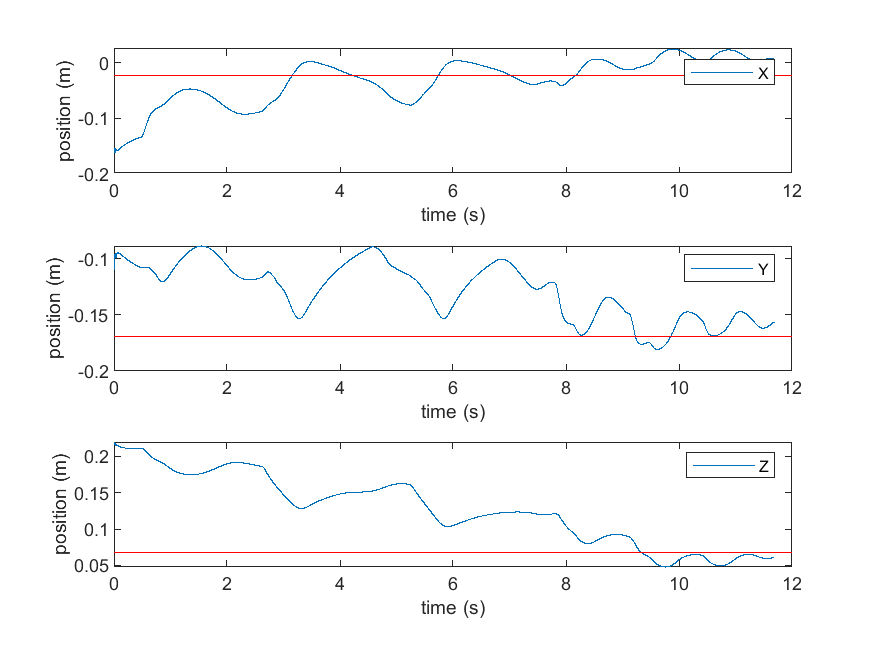
\includegraphics[width=\linewidth]{Pictures/Results/Controller/Stroke7/20.png}
        \caption{Example 2. Stroke=7.}
    \end{subfigure}
    
    \vspace{2pt} % Some vertical space between the rows
        \begin{subfigure}[b]{0.45\textwidth}
        \centering
        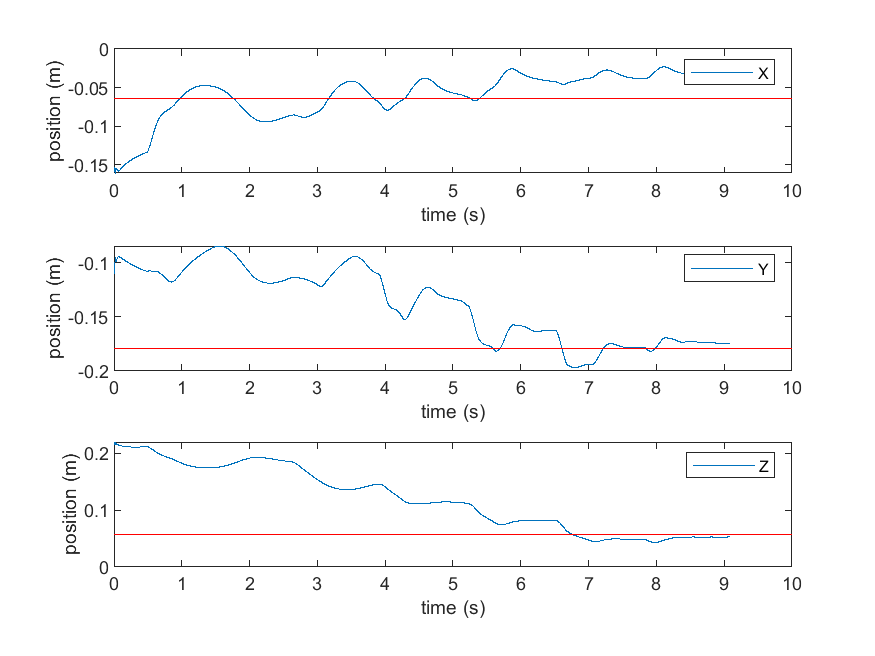
\includegraphics[width=\linewidth]{Pictures/Results/Controller/Stroke10/6.png}
        \caption{Example 1. Stroke=10.}
    \end{subfigure}%
    \hfill
    % Row 1, Column 2
    \begin{subfigure}[b]{0.45\textwidth}
        \centering
        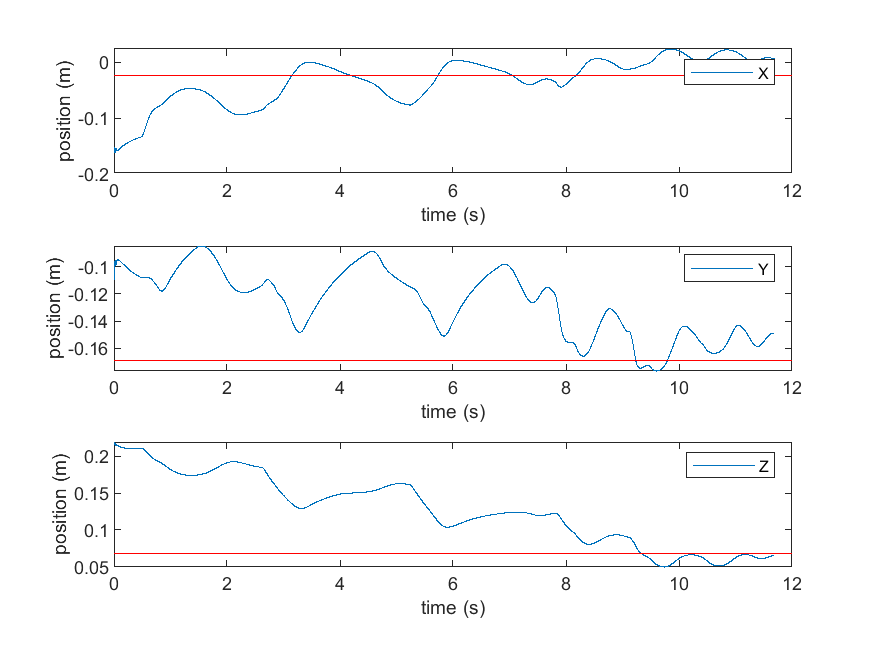
\includegraphics[width=\linewidth]{Pictures/Results/Controller/Stroke10/20.png}
        \caption{Example 1. Stroke=10.}
    \end{subfigure}
  
    \caption{Comparison for different stroke values of Wrist Position 2D with FES Controller}

\end{figure}
    


\newpage
\begin{landscape}
    \begin{figure}[ht]
        \centering
        % Row 1, Column 1
        \begin{subfigure}[b]{0.33\textwidth}
            \centering
            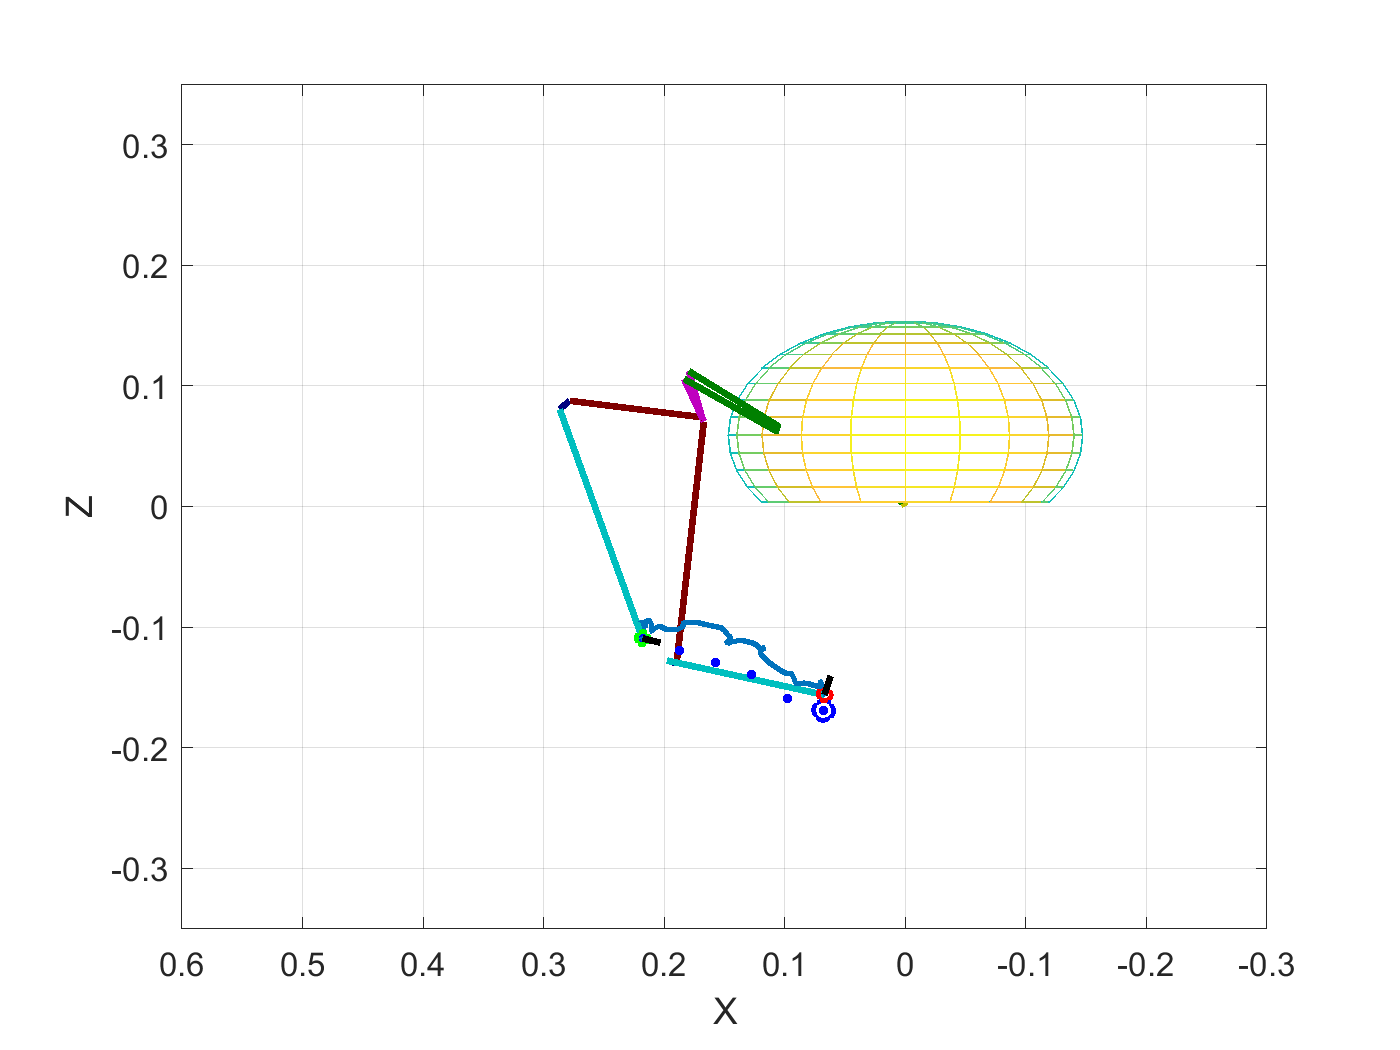
\includegraphics[width=\linewidth]{Pictures/Results/Controller/Stroke3/20_wp_nofes.png}
            \caption{Stroke=3. Wrist Position 3D without FES Controller}
        \end{subfigure}%
        \hfill
        % Row 1, Column 2
        \begin{subfigure}[b]{0.33\textwidth}
            \centering
            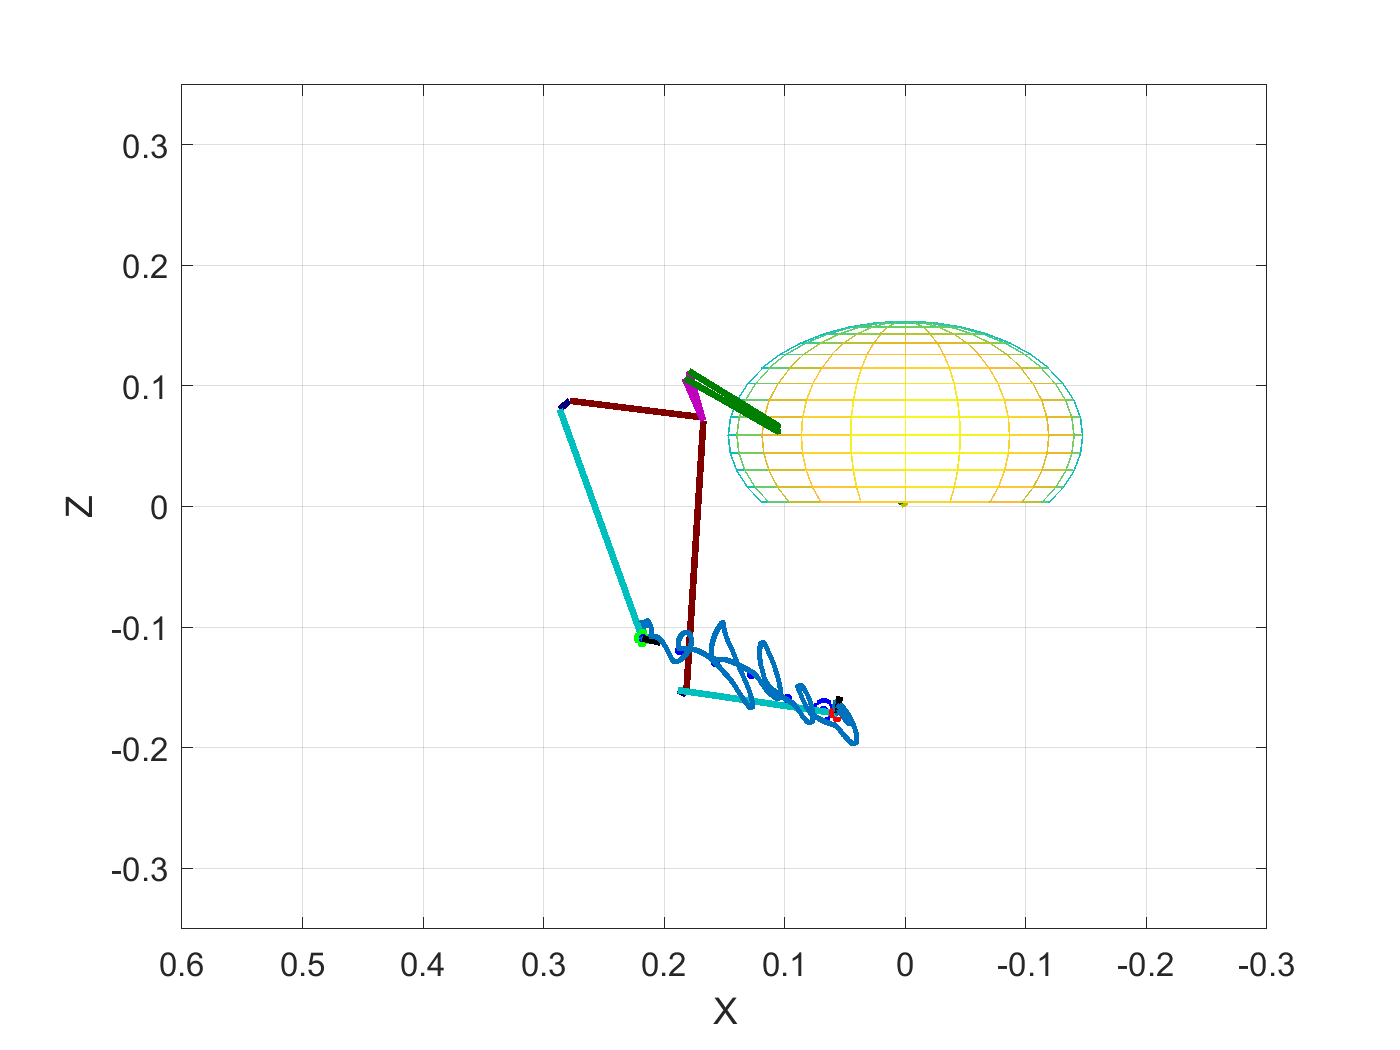
\includegraphics[width=\linewidth]{Pictures/Results/Controller/Stroke3/20_wp_fes.png}
            \caption{Stroke=3. Wrist Position 3D with FES Controller}
        \end{subfigure}
        \hfill
        \begin{subfigure}[b]{0.33\textwidth}
            \centering
            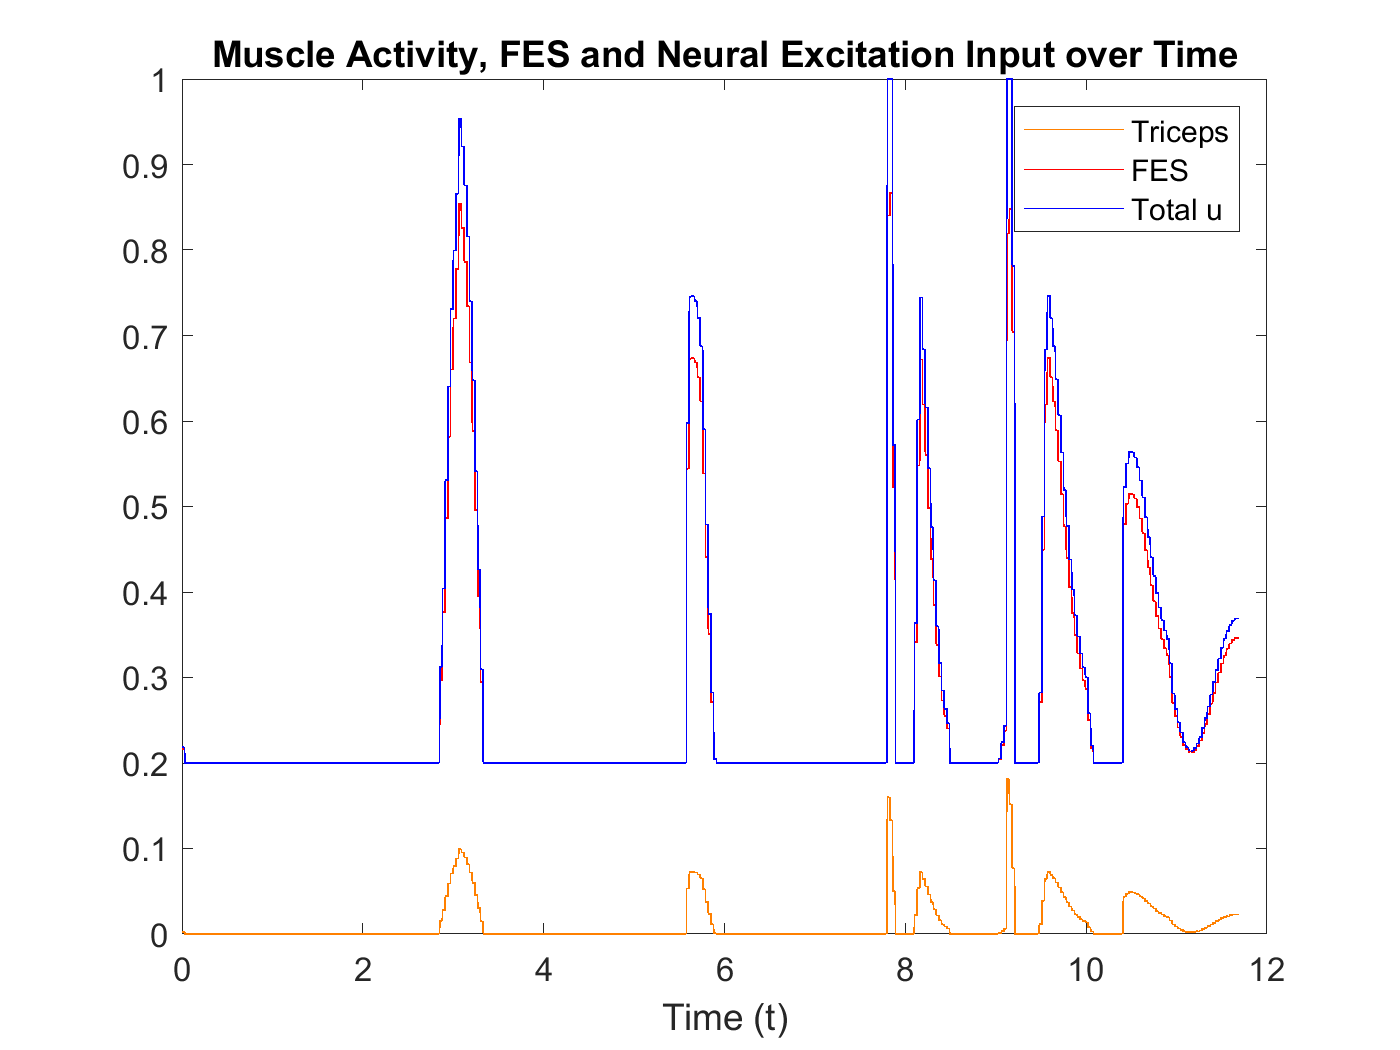
\includegraphics[width=\linewidth]{Pictures/Results/Controller/Stroke3/20_fes.png}
            \caption{Stroke=3. FES Excitation, Muscle Activity and Total Excitation}
        \end{subfigure}
        
        \vspace{2pt} % Some vertical space between the rows
    
        \begin{subfigure}[b]{0.33\textwidth}
            \centering
            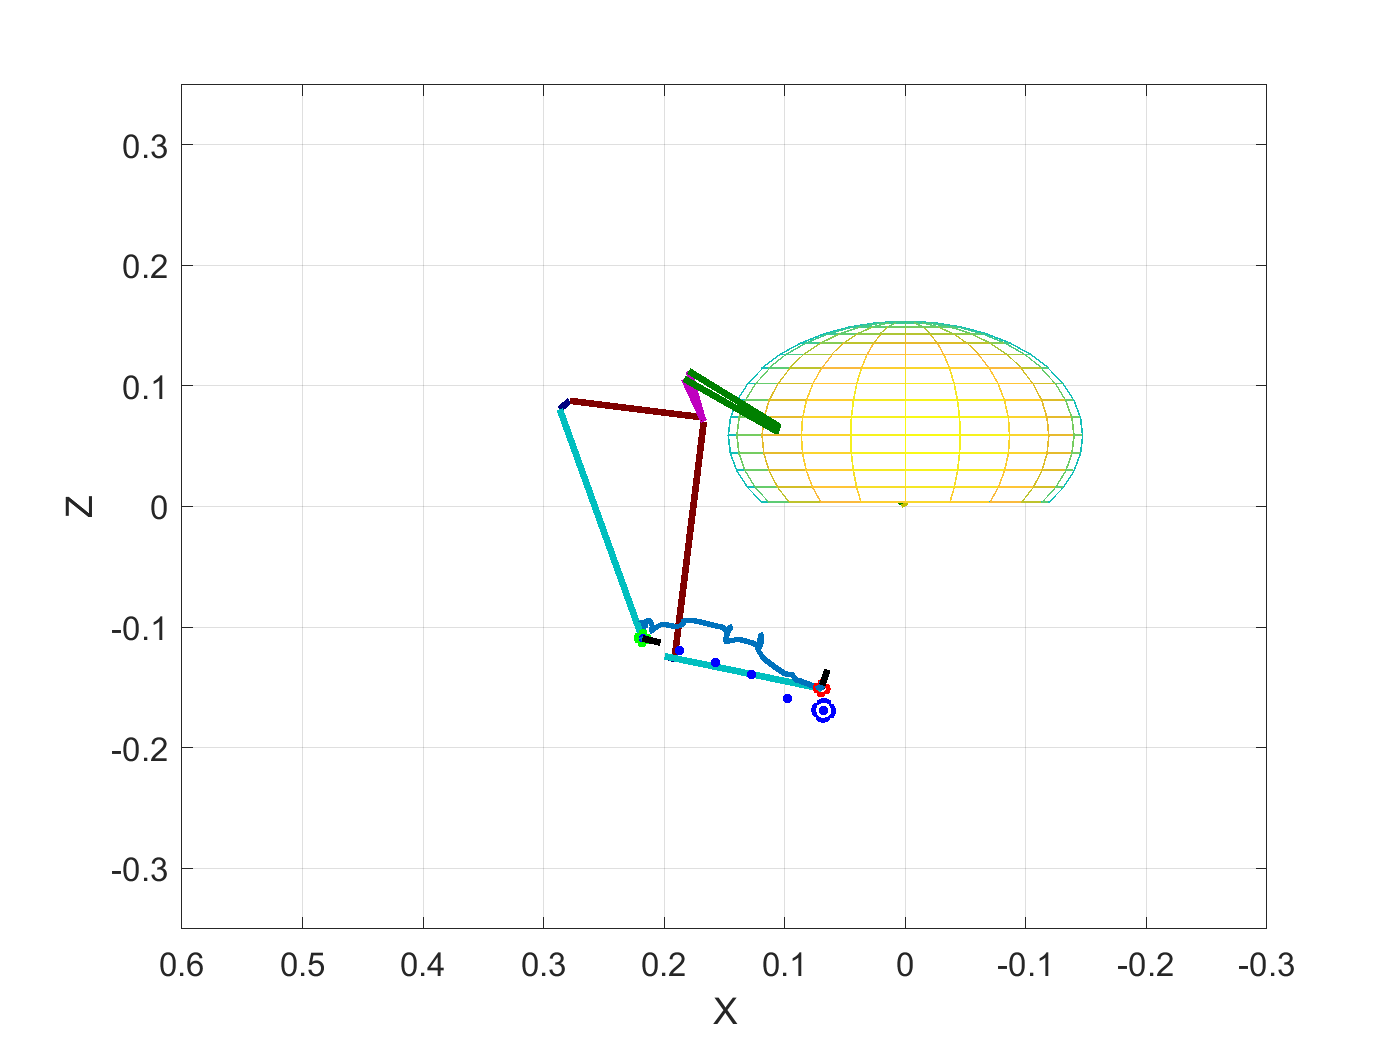
\includegraphics[width=\linewidth]{Pictures/Results/Controller/Stroke7/20_wp_nofes.png}
            \caption{Stroke=7. Wrist Position 3D without FES Controller}
        \end{subfigure}%
        \hfill
        % Row 1, Column 2
        \begin{subfigure}[b]{0.33\textwidth}
            \centering
            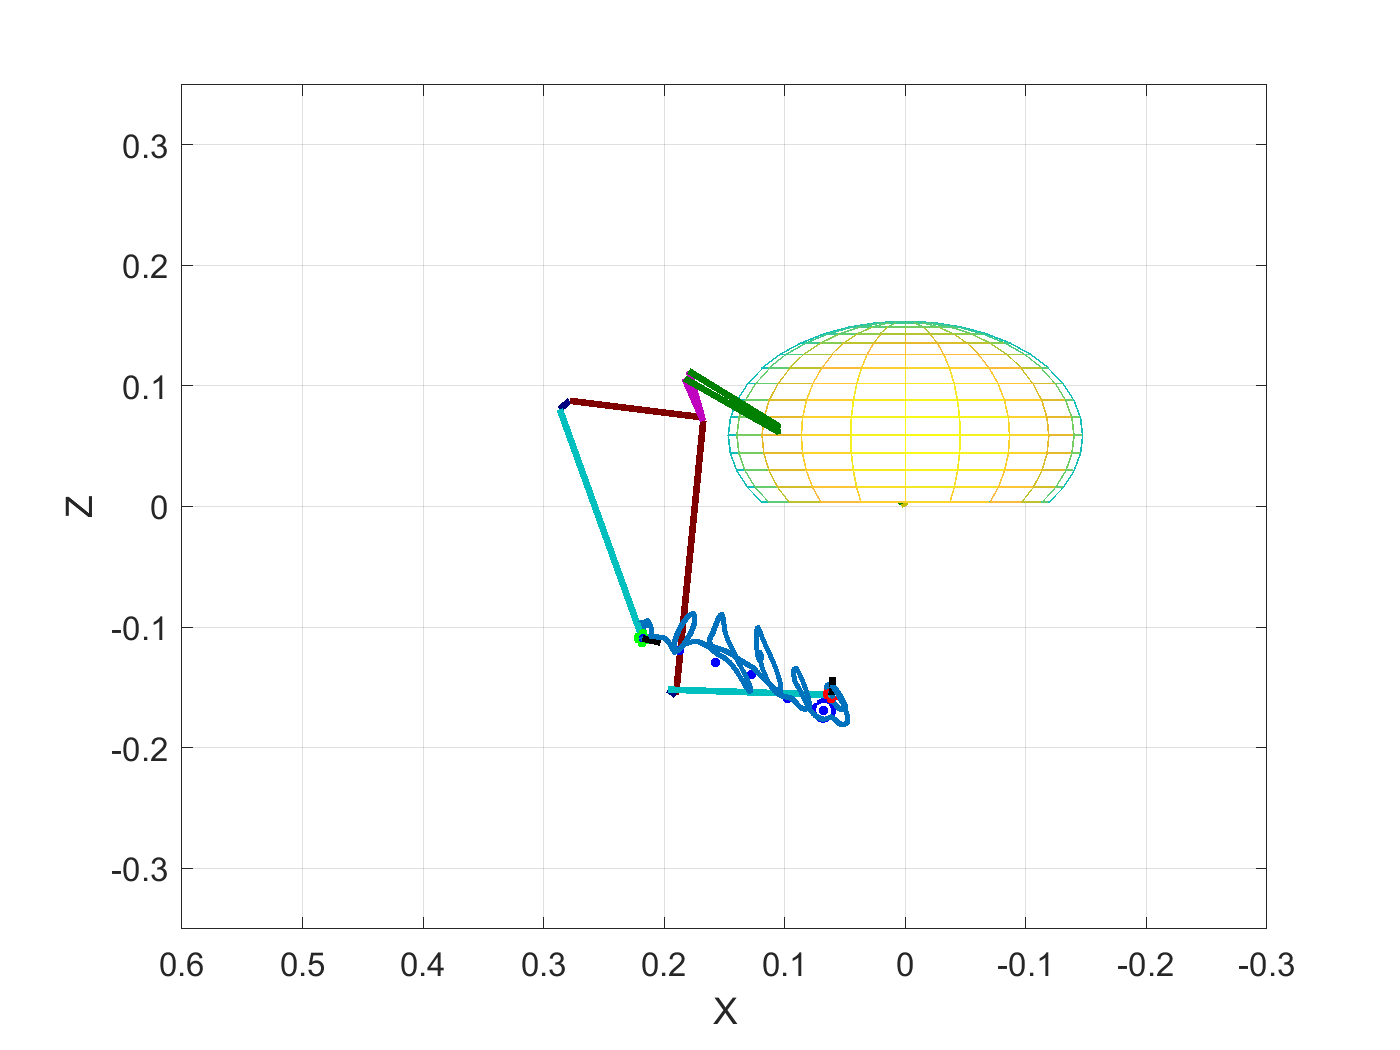
\includegraphics[width=\linewidth]{Pictures/Results/Controller/Stroke7/20_wp_fes.png}
            \caption{Stroke=7. Wrist Position 3D with FES Controller}
        \end{subfigure}
        \hfill
        \begin{subfigure}[b]{0.33\textwidth}
            \centering
            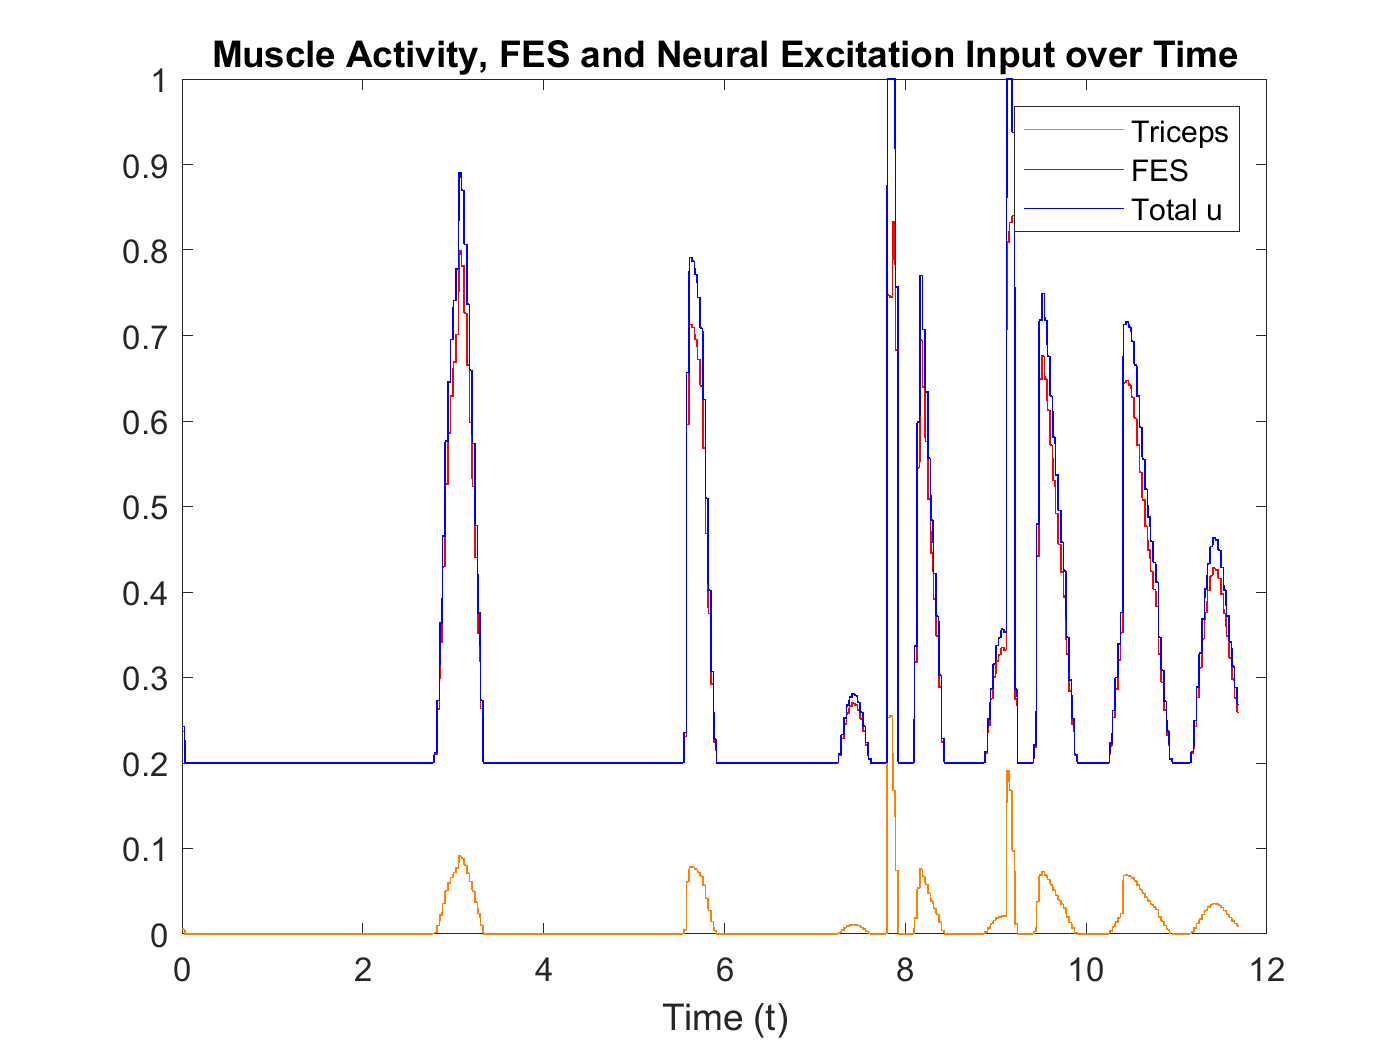
\includegraphics[width=\linewidth]{Pictures/Results/Controller/Stroke7/20_fes.png}
            \caption{Stroke=7. FES Excitation, Muscle Activity and Total Excitation}
        \end{subfigure}
        
        \vspace{2pt}

        \begin{subfigure}[b]{0.33\textwidth}
            \centering
            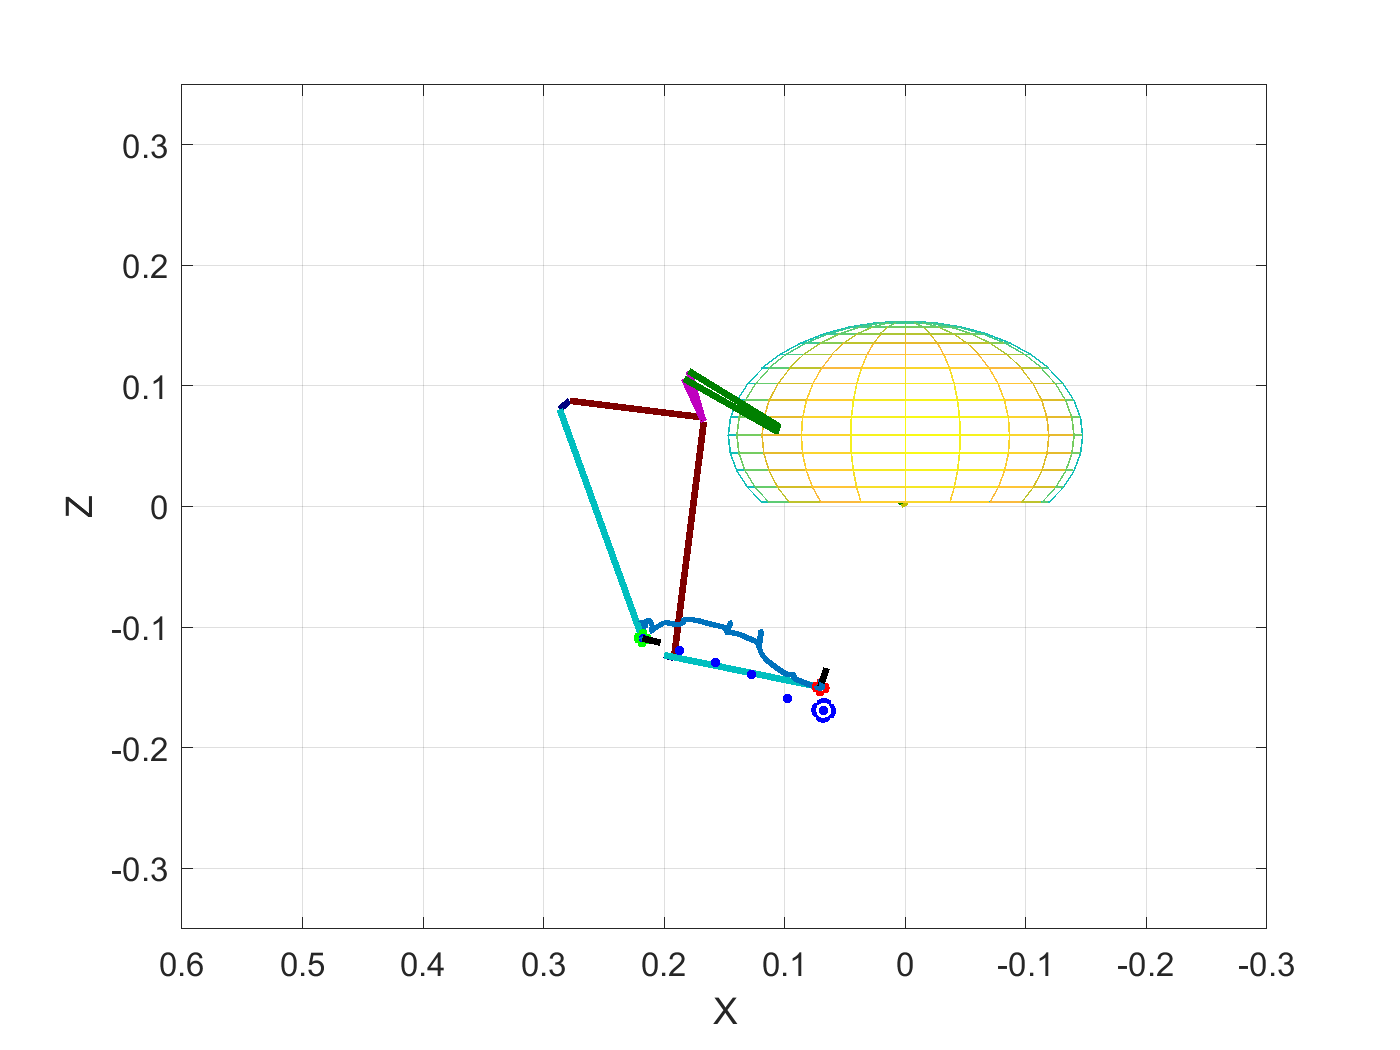
\includegraphics[width=\linewidth]{Pictures/Results/Controller/Stroke10/20_wp_nofes.png}
            \caption{Stroke=10. Wrist Position 3D without FES Controller}
        \end{subfigure}%
        \hfill
        % Row 1, Column 2
        \begin{subfigure}[b]{0.33\textwidth}
            \centering
            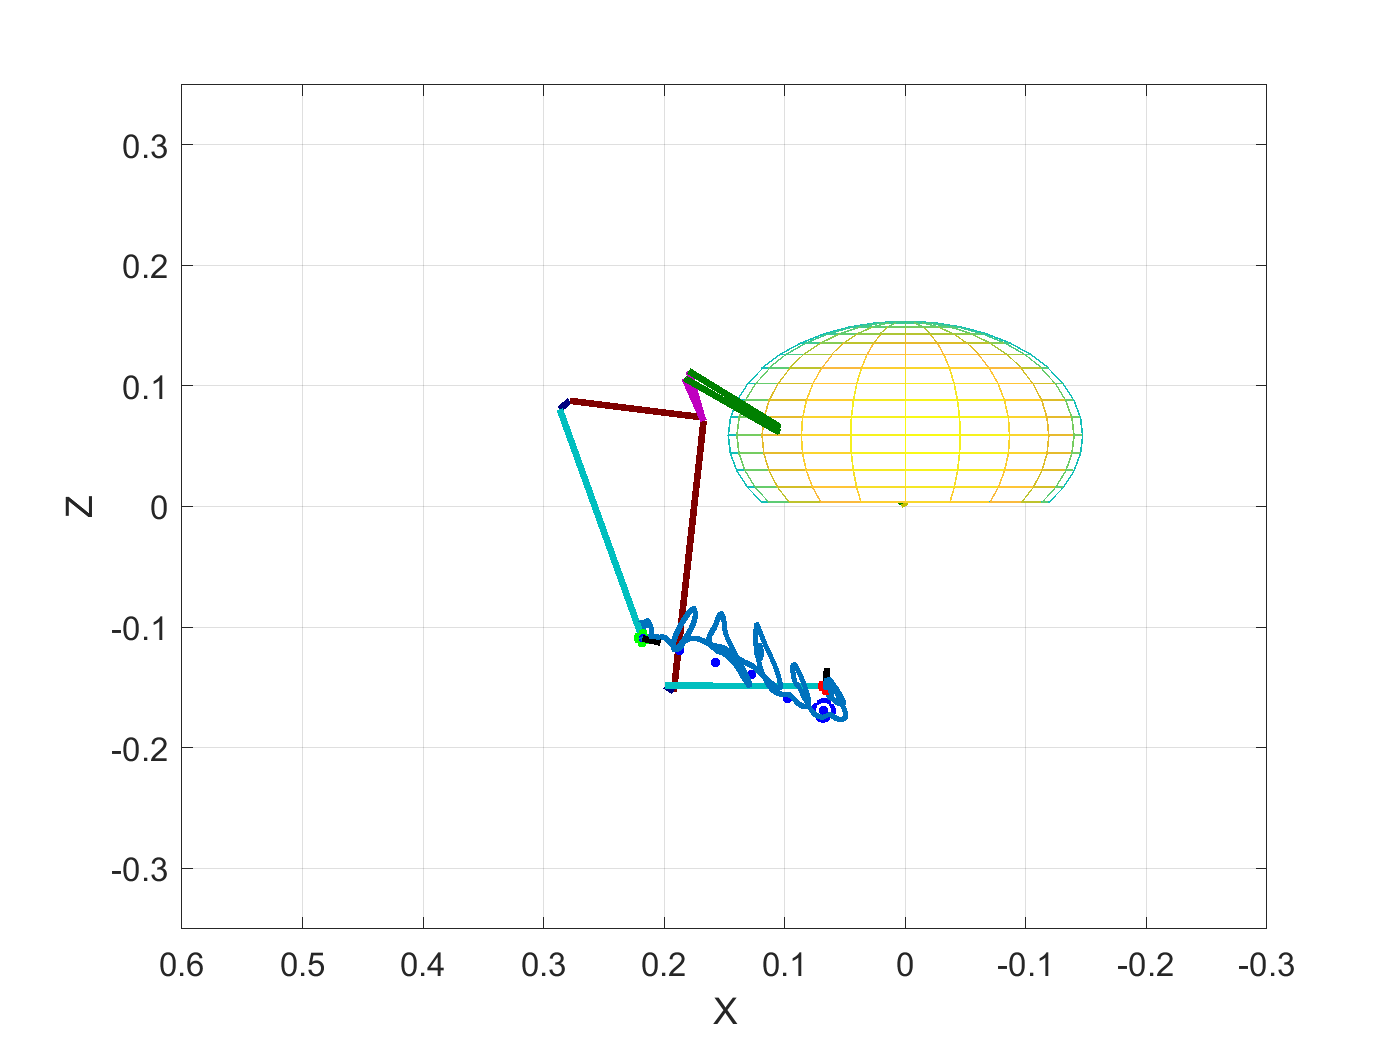
\includegraphics[width=\linewidth]{Pictures/Results/Controller/Stroke10/20_wp_fes.png}
            \caption{Stroke=10. Wrist Position 3D with FES Controller}
        \end{subfigure}
        \hfill
        \begin{subfigure}[b]{0.33\textwidth}
            \centering
            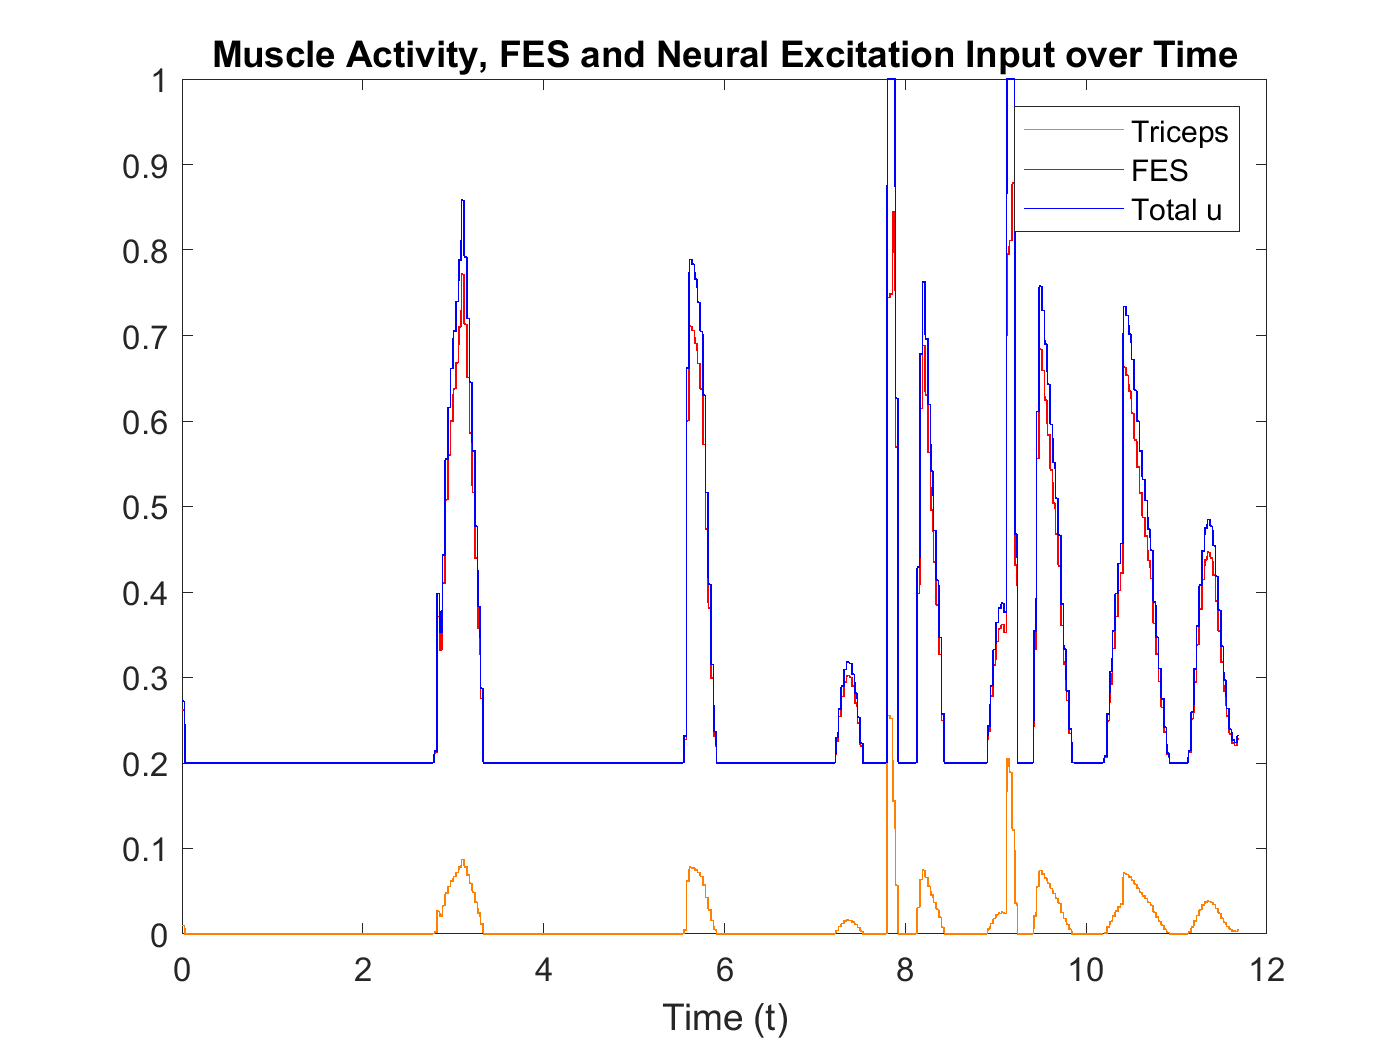
\includegraphics[width=\linewidth]{Pictures/Results/Controller/Stroke10/20_fes.png}
            \caption{Stroke=10. FES Excitation, Muscle Activity and Total Excitation}
        \end{subfigure}
            
        \caption{Example 1: EMG-Inspired FES Controller for Different Stroke}
        \label{fig:Ex1FESControllerDifferentStrokes}
    \end{figure}
\end{landscape}

\newpage
\begin{landscape}
    \begin{figure}[ht]
        \centering
        % Row 1, Column 1
        \begin{subfigure}[b]{0.33\textwidth}
            \centering
            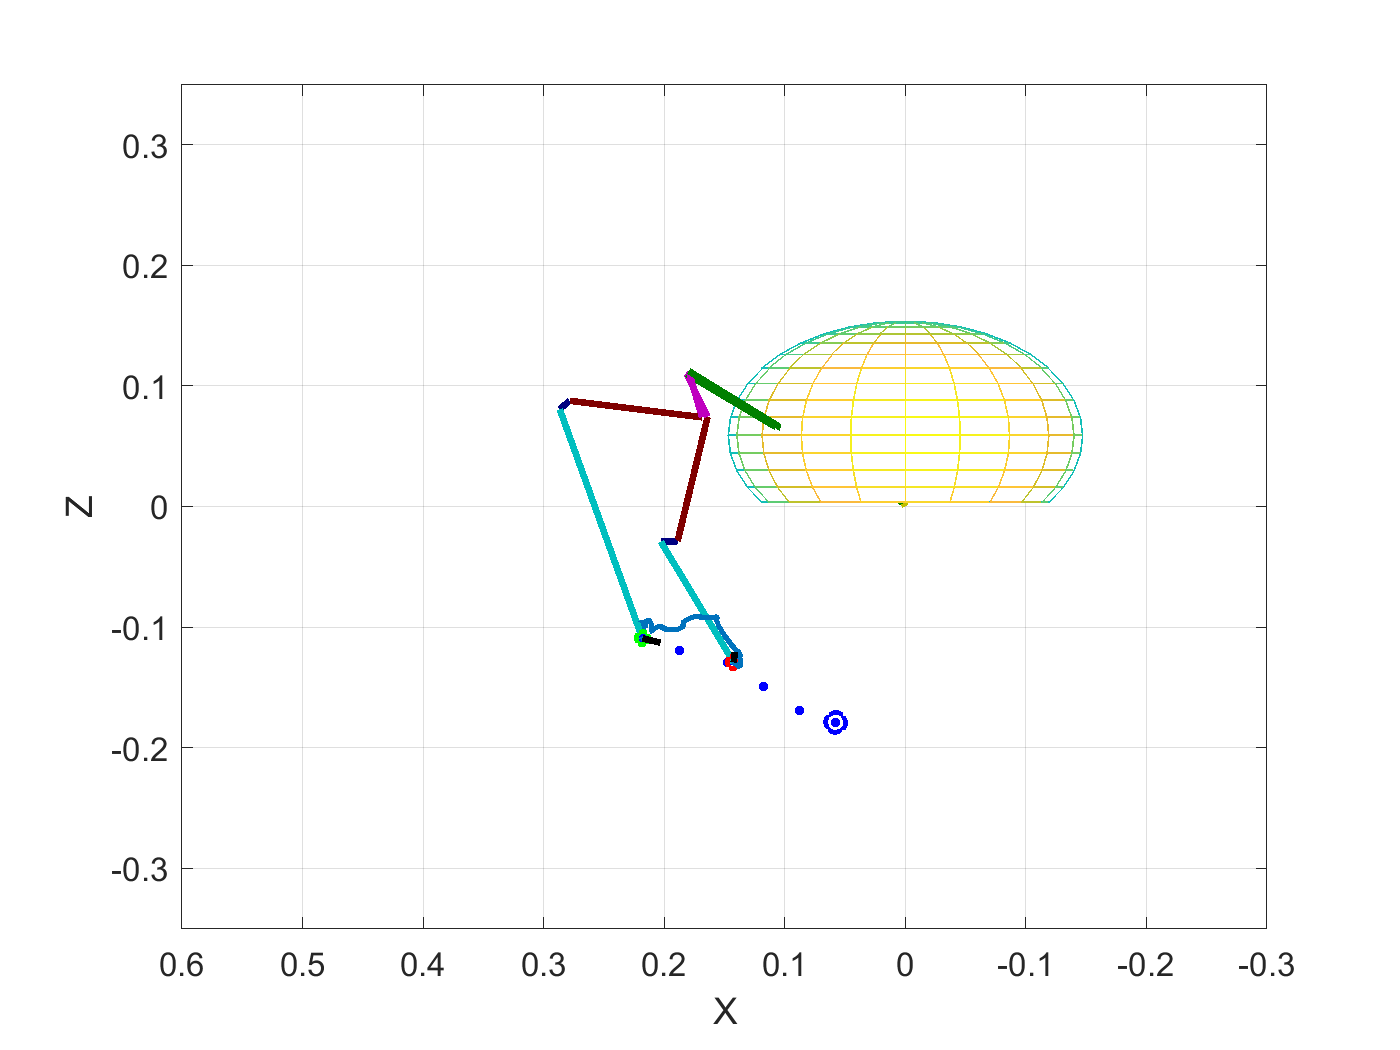
\includegraphics[width=\linewidth]{Pictures/Results/Controller/Stroke3/6_wp_nofes.png}
            \caption{Stroke=3. Wrist Position 3D without FES Controller}
        \end{subfigure}%
        \hfill
        % Row 1, Column 2
        \begin{subfigure}[b]{0.33\textwidth}
            \centering
            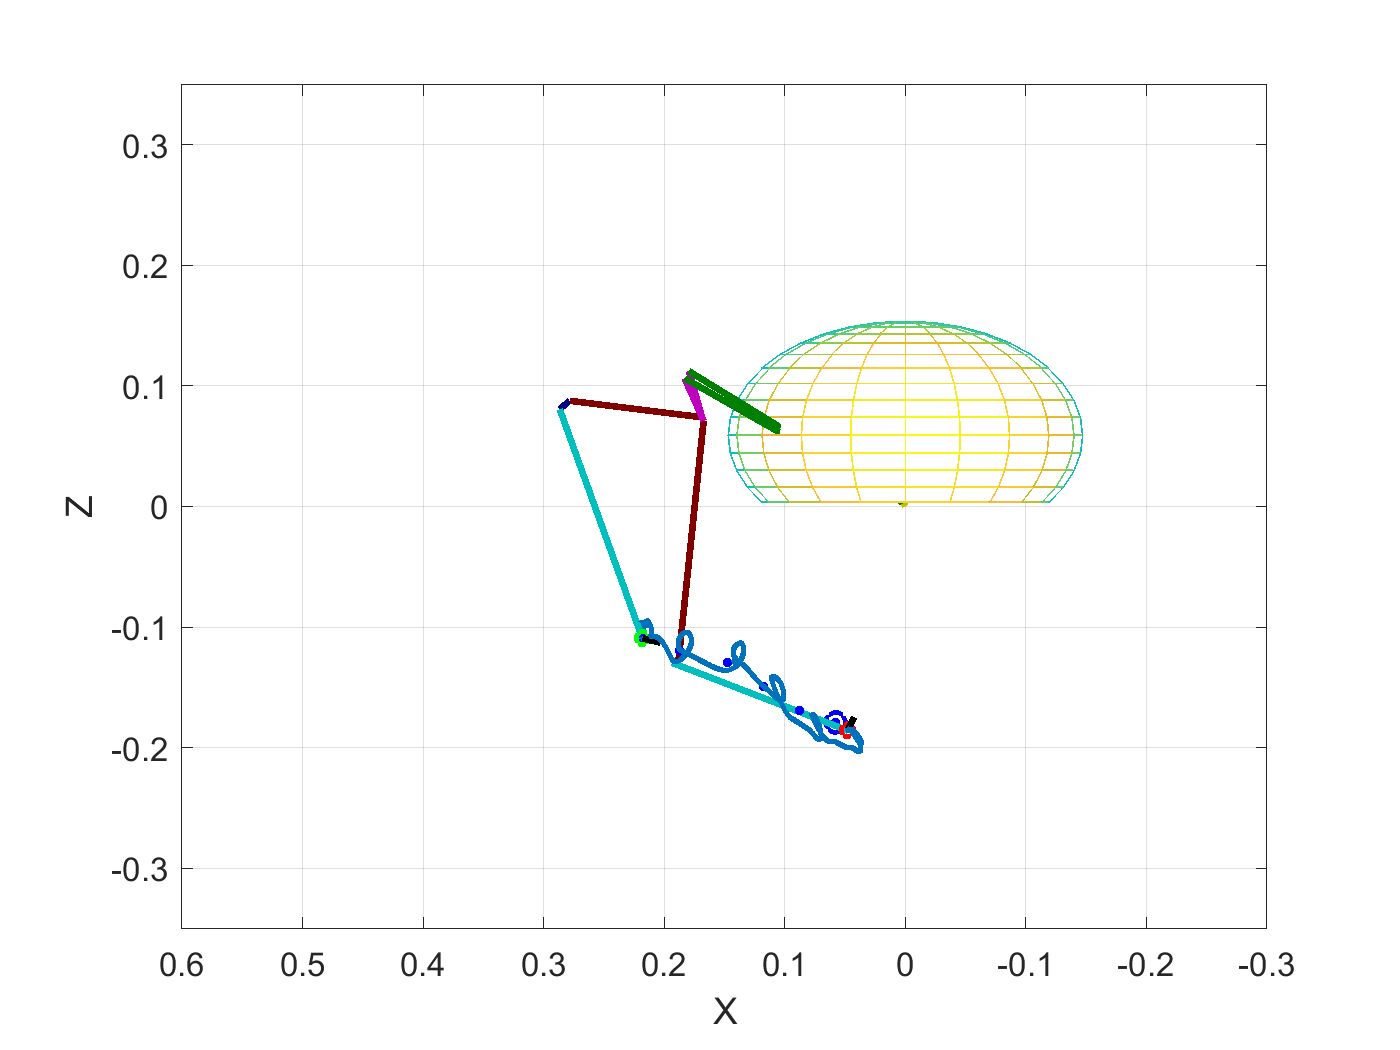
\includegraphics[width=\linewidth]{Pictures/Results/Controller/Stroke3/6_wp_fes.png}
            \caption{Stroke=3. Wrist Position 3D with FES Controller}
        \end{subfigure}
        \hfill
        \begin{subfigure}[b]{0.33\textwidth}
            \centering
            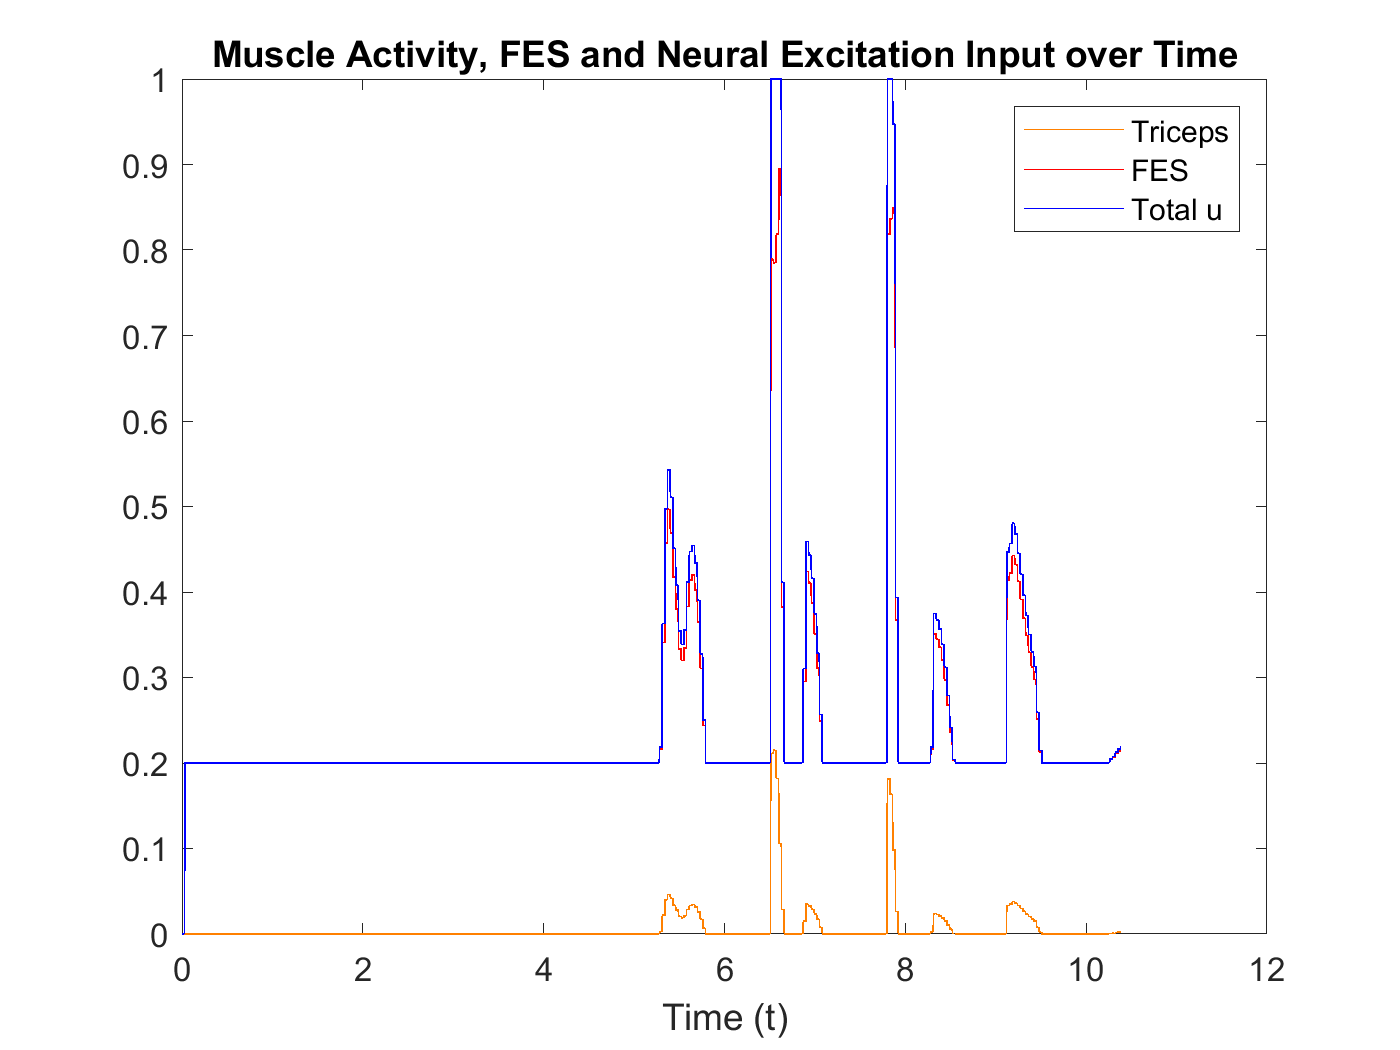
\includegraphics[width=\linewidth]{Pictures/Results/Controller/Stroke3/6_fes.png}
            \caption{Stroke=3. FES Excitation, Muscle Activity and Total Excitation}
        \end{subfigure}
        
        \vspace{2pt} % Some vertical space between the rows
    
        \begin{subfigure}[b]{0.33\textwidth}
            \centering
            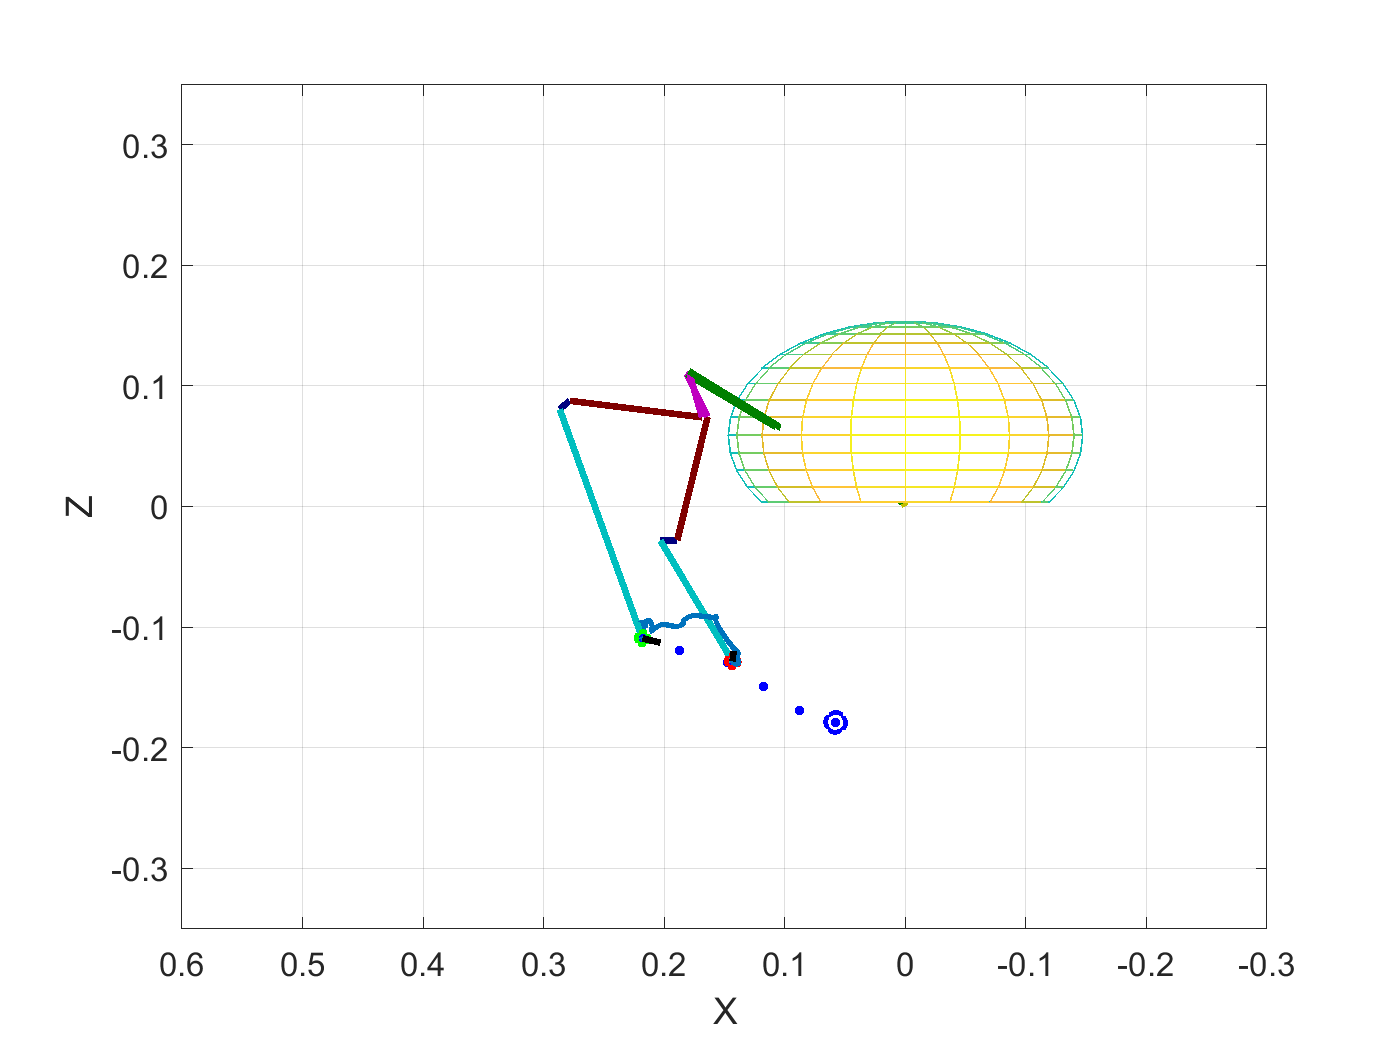
\includegraphics[width=\linewidth]{Pictures/Results/Controller/Stroke7/6_wp_nofes.png}
            \caption{Stroke=7. Wrist Position 3D without FES Controller}
        \end{subfigure}%
        \hfill
        % Row 1, Column 2
        \begin{subfigure}[b]{0.33\textwidth}
            \centering
            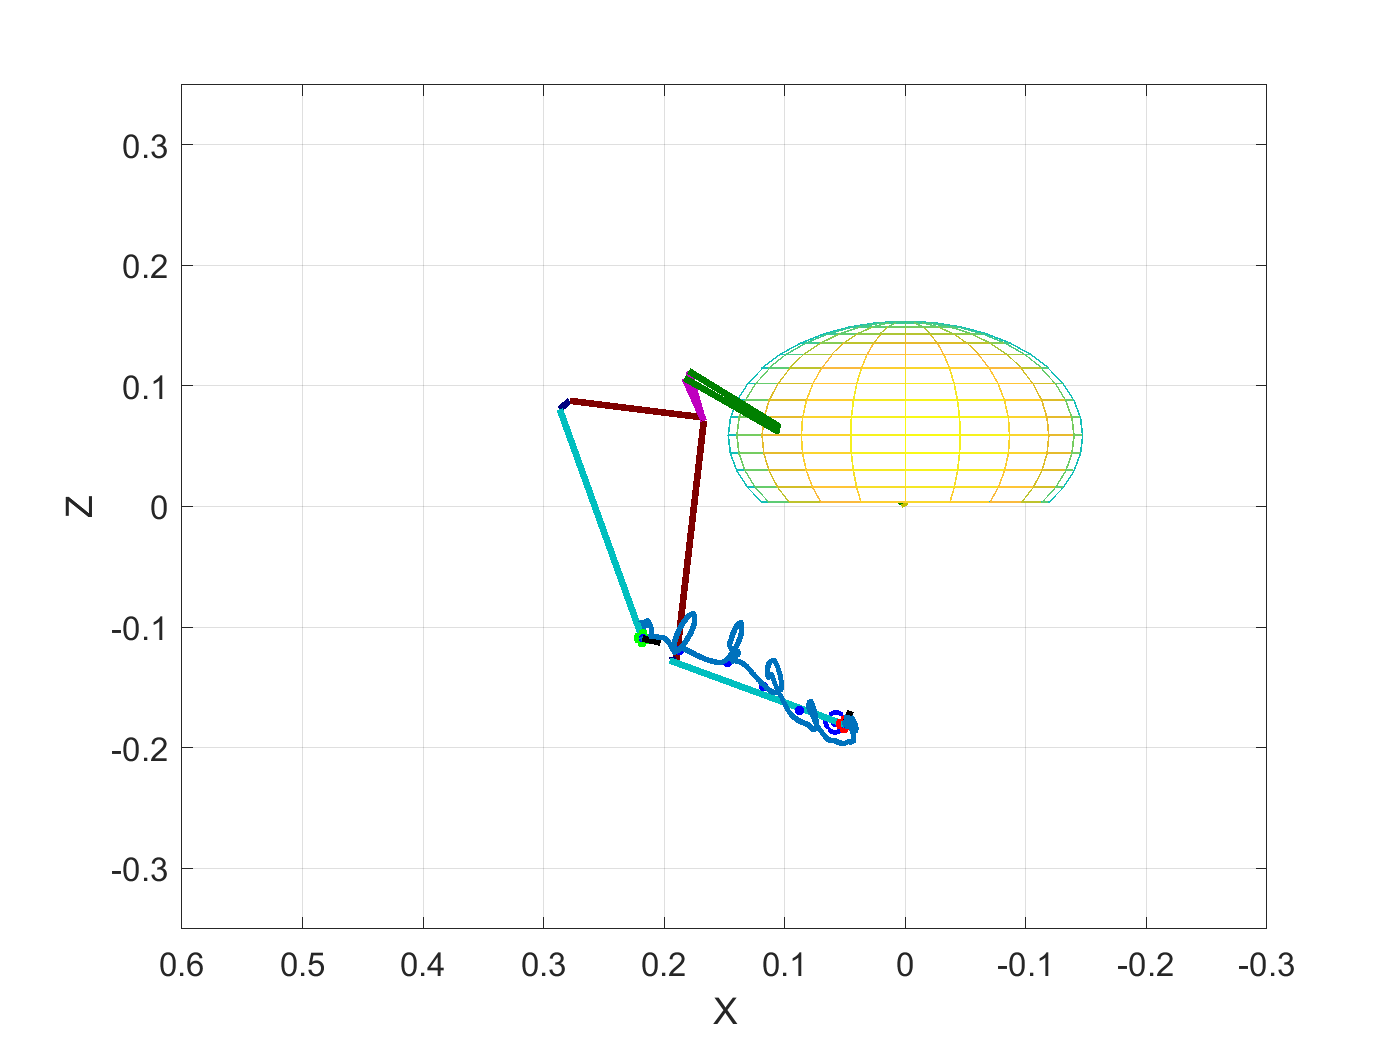
\includegraphics[width=\linewidth]{Pictures/Results/Controller/Stroke7/6_wp_fes.png}
            \caption{Stroke=7. Wrist Position 3D with FES Controller}
        \end{subfigure}
        \hfill
        \begin{subfigure}[b]{0.33\textwidth}
            \centering
            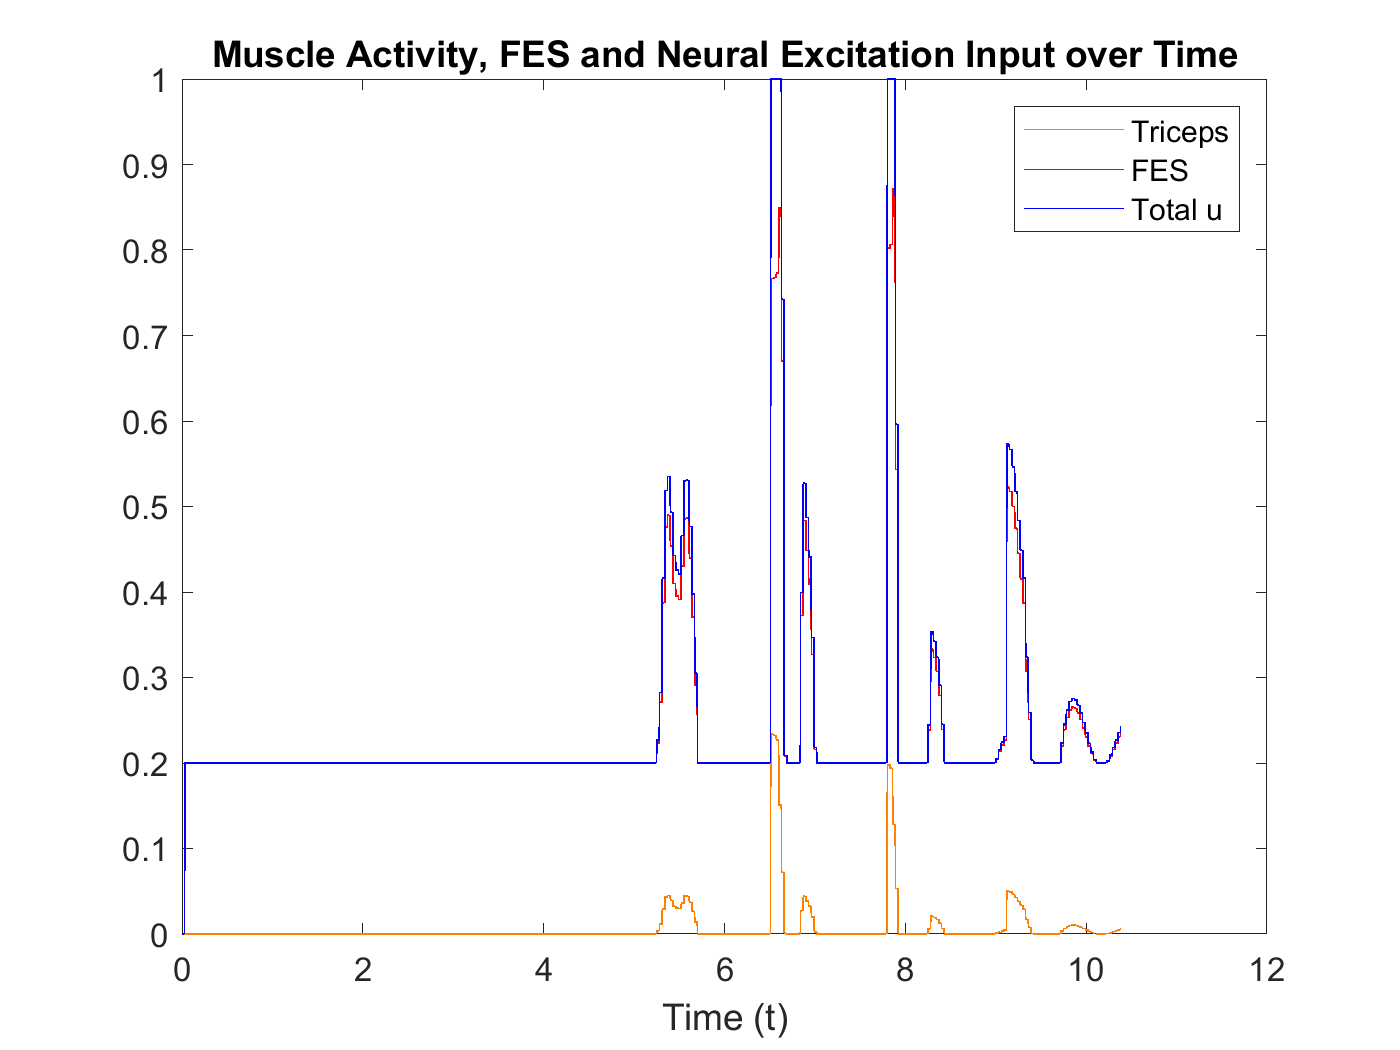
\includegraphics[width=\linewidth]{Pictures/Results/Controller/Stroke7/6_fes.png}
            \caption{Stroke=7. FES Excitation, Muscle Activity and Total Excitation}
        \end{subfigure}
        
        \vspace{2pt}

        \begin{subfigure}[b]{0.33\textwidth}
            \centering
            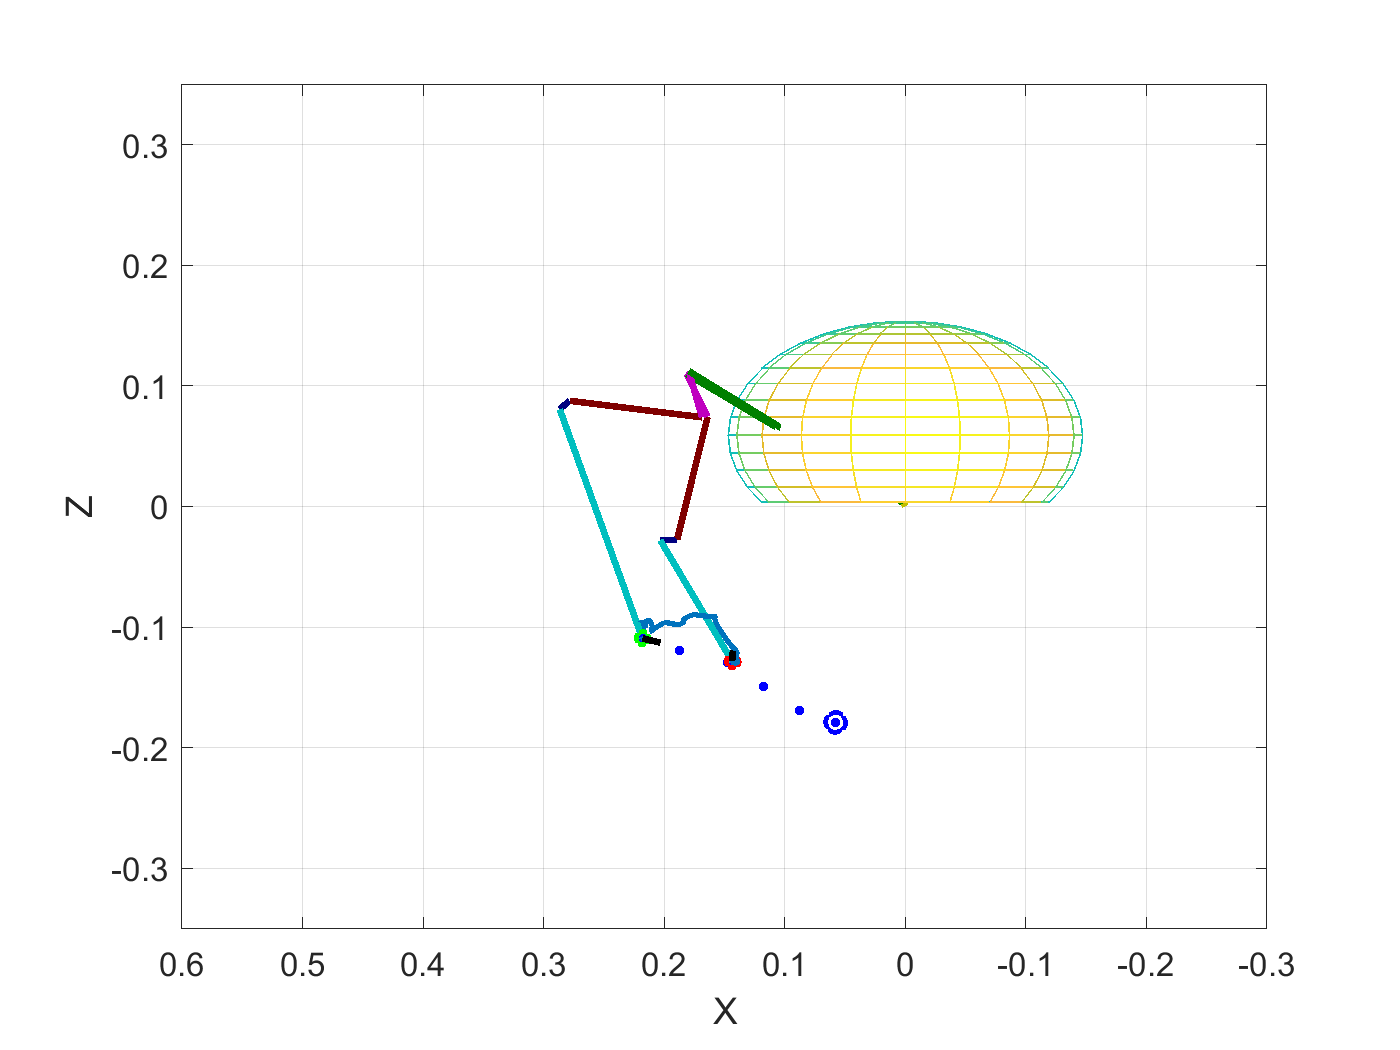
\includegraphics[width=\linewidth]{Pictures/Results/Controller/Stroke10/6_wp_nofes.png}
            \caption{Stroke=10. Wrist Position 3D without FES Controller}
        \end{subfigure}%
        \hfill
        % Row 1, Column 2
        \begin{subfigure}[b]{0.33\textwidth}
            \centering
            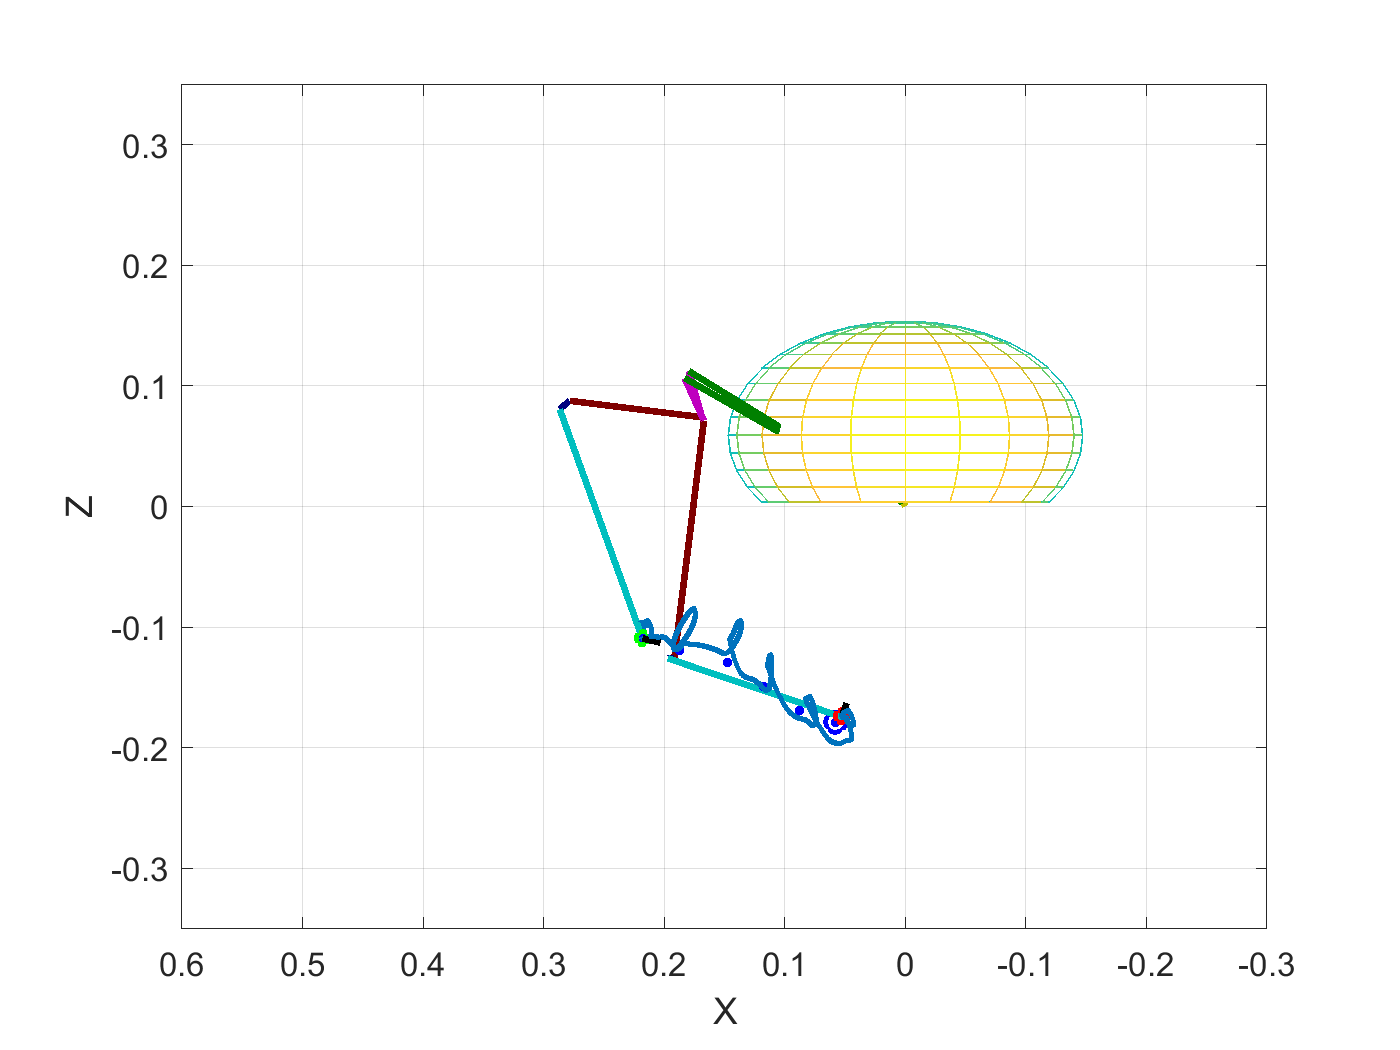
\includegraphics[width=\linewidth]{Pictures/Results/Controller/Stroke10/6_wp_fes.png}
            \caption{Stroke=10. Wrist Position 3D with FES Controller}
        \end{subfigure}
        \hfill
        \begin{subfigure}[b]{0.33\textwidth}
            \centering
            \includegraphics[width=\linewidth]{Pictures/Results/Controller/Stroke10/6_fes.png}
            \caption{Stroke=10. FES Excitation, Muscle Activity and Total Excitation}
        \end{subfigure}
            
        \caption{Example 2: EMG-Inspired FES Controller for Different Stroke}
        \label{fig:Ex2FESControllerDifferentStrokes}
    \end{figure}
\end{landscape}

\newpage
\begin{landscape} % Start landscape page
  \begin{figure}[h!]
    \centering
    \includegraphics[width=1.9\textwidth]{Pictures/Results/Controller/WithStroke29positions.png} % Replace "filename.jpg" with the name of your image file
    \caption{Desired Targets With Stroke = 7 Without EMG-Influenced Control} % Optional caption
  \end{figure}
\end{landscape} % End landscape page



\newpage
\begin{landscape} % Start landscape page
  \begin{figure}[h!]
    \centering
    \includegraphics[width=1.9\textwidth]{Pictures/Results/Controller/Stroke29positions.png}
    \caption{Desired Targets With Stroke = 7 With EMG-Influenced Control} 
  \end{figure}
\end{landscape} % End landscape page